%% Il y a deux façons d'utiliser ce prototype de thèse:
%%       soit vous pouvez pas blairer LaTeX,
%%       soit vous en êtes un gourou.
%% Dans le premier cas, il vous suffira de remplacer ce qu'il faut 
%% dans ce fichier pour obtenir presque automatiquement un manuscript qui 
%% ressemble à une thèse réglementaire.
%%
%% Dans le second cas, vous ne pourrez vous empêcher d'aller trafiquer
%% le fichier these.sty pour rendre les choses encore plus automatiques
%% (il y a sûrement un moyen de rendre plus élégante la mise en place 
%% du résumé sur la quatrième de couverture, par exemple)
%% et l'adapter aux derniers caprices de la Scolarité. 
%% SVP, dans ce cas, faites profiter tout le monde de vos améliorations
%% en renvoyant these.sty et un exemple de these.tex au ouaibemestre de l'ADOC.
%%
 
\documentclass[11pt]{book}
%% En 12pt c'est possible aussi

%% packages utilises
%%---------------------

\usepackage{listings}

\lstdefinelanguage{javamine}
  {morekeywords=[0]{then, end, operation, is, abstract,boolean,break,byte,case,catch,char,class,
      const,continue,default,do,double,else,extends,false,final,
      finally,float,for,goto,if,init, implements,import,instanceof,int,
      interface,label,long,native,new,null,package,private,protected,
      public,return,result,short,static,super,switch,synchronized,this,throw,
      throws,transient,true,try,void,volatile,while, val, var, def, foreach, filter},
      morekeywords=[1]{name,className,type,libName, exists, each},%
      morekeywords=[2]{@ComponentType,@Start,@Stop,@Update,@ProvidedPort,@Provides,@RequiredPort,@Requires,@DictionaryType,@Port,@Ports,@Library,@DictionaryAttribute},%
   sensitive,%
   morecomment=[l]//,%
   morecomment=[s]{/*}{*/},%
   morestring=[b]",%
   morestring=[b]',%
  }[keywords,comments,strings]%

\usepackage{color}

\definecolor{colKeys}{rgb}{0,0,1} 
\definecolor{colIdentifier}{rgb}{0,0,0} 
\definecolor{colComments}{rgb}{0,0.5,1} 
\definecolor{colString}{rgb}{0.6,0.1,0.1} 
\definecolor{DGreen}{rgb}{0,0.5,0} 
\lstset{language=javamine,basicstyle=\ttfamily\small, % 
identifierstyle=\color{colIdentifier}, % 
keywordstyle=[0]\bf\color{colKeys},
keywordstyle=[1]\bf\color{black},
keywordstyle=[2]\color{DGreen}, % 
stringstyle=\color{colString}, % 
commentstyle=\color{colComments},
showstringspaces=false
} 

\lstset{language=javamine, frame=single, backgroundcolor=\color{LGrey}}


%\usepackage{lstlang3}

\usepackage[utf8]{inputenc}
\usepackage[T1]{fontenc}
\usepackage[english,frenchb]{babel}
%\usepackage{amsmath}
%\usepackage{math}
%\usepackage{amssymb}
\usepackage{these}
\usepackage{array}
\usepackage{rotating}
 	
\usepackage{tabularx}
%\usepackage{epsfig, floatflt,amssymb} 
%\usepackage{moreverb} %% pour le verbatim en boite
%\usepackage{slashbox} %% pour couper les colonnes des tableaux en diagonale 
%\usepackage{showkeys} %% pour voir les labels
\usepackage{multirow} %% pour regrouper un texte sur plusieurs lignes dans une table
\usepackage{url} %% pour citer les url par \url
%\usepackage[all]{xy} %% pour la barre au dessus des symboles
%\usepackage{shorttoc} %% pour plusieurs tables des matières par la commande \shorttableofcontents{Titre}{profondeur}.
%\usepackage{textcomp} %% pour le symbol pour mille par \textperthousand.
%\usepackage{hyperref} %% pour la transformation en PDF, ça permet d'obtenir des liens sur les sections ...
%\usepackage{bookmark}

%\usepackage[pdftex,bookmarks=true,hypertexnames=false]{hyperref}
\usepackage[bookmarks=true,hypertexnames=false]{hyperref}
\usepackage[acronym]{glossaries}
%\bookmarksetup{startatroot}
%\usepackage{comment}

%\usepackage{textcomp}
\usepackage{eurosym}
\DeclareUnicodeCharacter{20AC}{\euro}
%\usepackage{eurosans} %%pour le symbole \euro
%\usepackage{epic,eepic}
%\usepackage{times}%times,palatino}
%\usepackage{palatino}
%\usepackage{helvetica} : tjrs le pb
%\usepackage{utopia}:pb de cesure
%Manipulation TOC
\usepackage{tocloft}

\usepackage{subfig}
\usepackage{wrapfig}

%% macro/racourcis por les symboles et commandes usuelles
%\input{./macro}

%% choix des profondeurs de section pour la table des matières
%% 2= subsection, 3=subsubsection
%\setcounter{secnumdepth}{3}  %% Avec un numero.
%\setcounter{tocdepth}{4}     %% Visibles dans la table des matieres
%mode plan
% \makeatletter
% \renewcommand*\l@part[2]{%
%   \ifnum \c@tocdepth >-2\relax
%     \addpenalty{-\@highpenalty}%
%     \addvspace{2.25em \@plus\p@}%
%     \setlength\@tempdima{3em}%
%     \begingroup
%       \parindent \z@ \rightskip \@pnumwidth
%       \parfillskip -\@pnumwidth
%       {\leavevmode
%        \rm\color{black}\def\@linkcolor{black}%
%        \large\bfseries{\mathversion{bold}#1}\hfil
%        \hb@xt@\@pnumwidth{\hss
%        \def\@linkcolor{black}\color{black}#2}}\par
%        \nobreak
%          \global\@nobreaktrue
%          \everypar{\global\@nobreakfalse\everypar{}}%
%     \endgroup
%   \fi}
% \renewcommand*\l@chapter[2]{%
%   \ifnum \c@tocdepth >\m@ne
%     \addpenalty{-\@highpenalty}%
%     \vskip 1.0em \@plus\p@
%     \setlength\@tempdima{1.5em}%
%     \begingroup
%       \parindent \z@ \rightskip \@pnumwidth
%       \parfillskip -\@pnumwidth
%       \leavevmode \bfseries
%       \advance\leftskip\@tempdima
%       \hskip -\leftskip
%       \def\@linkcolor{black}%
%       \rm\color{black}{\mathversion{bold}#1}\nobreak\
%        \leaders\hbox{$\m@th
%         \mkern \@dotsep mu\hbox{.}\mkern \@dotsep
%         mu$}\hfil\nobreak\hb@xt@\@pnumwidth{\hss
%         \def\@linkcolor{black}%
%         \rm\color{black}#2}\par
%       \penalty\@highpenalty
%     \endgroup
%   \fi}
% \def\@dottedtocline#1#2#3#4#5{%
%   \ifnum #1>\c@tocdepth \else
%     \vskip \z@ \@plus.2\p@
%     {\leftskip #2\relax \rightskip \@tocrmarg \parfillskip -\rightskip
%      \parindent #2\relax\@afterindenttrue
%      \interlinepenalty\@M
%      \leavevmode
%      \@tempdima #3\relax
%      \advance\leftskip \@tempdima \null\nobreak\hskip -\leftskip
%      {#4}\nobreak
%      \leaders\hbox{$\m@th
%         \mkern \@dotsep mu\hbox{.}\mkern \@dotsep
%         mu$}\hfill
%      \nobreak
%      \hb@xt@\@pnumwidth{\hfil\normalfont #5}%
%      \par}%
%   \fi}
% %\renewcommand*\l@part{\rm\color{black}\def\@linkcolor{black}\@dottedtocline{1}{1.5em}{2.3em}}
% %\renewcommand*\l@chapter{\rm\color{black}\def\@linkcolor{black}\@dottedtocline{1}{1.5em}{2.3em}}
% \renewcommand*\l@section{\rm\color{black}\def\@linkcolor{black}\@dottedtocline{1}{1.5em}{2.3em}}
% \renewcommand*\l@paragraph{\bf}
% \makeatother

%\setlength{\cftparaindent}{\cftsubsecindent}
%\renewcommand{\cftparadotsep}{\cftnodots}
%\cftsetindents{para}{\cftsubsecindent}{0em}
%\cftpagenumbersoff{para}
%
%\renewcommand{\cftparafont}{\bfseries}
%\renewcommand{\cftparapagefont}{\bfseries}


\newcommand\enti{EnTiMid}
\definecolor{LGrey}{rgb}{0.95,0.95,0.95}
%\renewcommand{\thefigure}{\arabic{part}.\thechapter.\arabic{figure}}
\usepackage{tocloft}
\setlength{\cftfignumwidth}{3em}
%\makeatletter
%\renewcommand*{\l@paragraph}[2]{%
% \ifnum \c@tocdepth >3\relax
% \vskip \cftbeforeparaskip
% {\leftskip \cftparaindent\relax
% \rightskip \@tocrmarg
% \parfillskip -\rightskip
% \parindent \cftparaindent\relax\@afterindenttrue
% \interlinepenalty\@M
% \leavevmode
% \@tempdima \cftparanumwidth\relax
% \let\@cftbsnum \cftparapresnum
% \let\@cftasnum \cftparaaftersnum
% \let\@cftasnumb \cftparaaftersnumb
% \advance\leftskip \@tempdima \null\nobreak\hskip -\leftskip
% {\cftparafont \bf{#1}}\nobreak
% \cftparafillnum{#2}}%
% \fi}


\makeglossaries

\makeindex %% crée l'index

\renewcommand{\contentsname}{Table of contents}

\def\underscore{\char`\_}

%% c'est parti mon kiki !!
%%%%%%%%%%%%%%%%%%%%%%%%%%%%%%%%%%%%%%%%%%%
\begin{document}%%%%%%%%%%%%%%%%%%%%%%%%%%%
%%%%%%%%%%%%%%%%%%%%%%%%%%%%%%%%%%%%%%%%%%%

%%%%%%%%%%%%%%%%%%%%%%%%%
%       Acronims        %
%%%%%%%%%%%%%%%%%%%%%%%%%

%\newacronym{lvm}{LVM}{Logical Volume Manager}

\newacronym{aal}{AAL}{Ambient Assisted Living}
\newacronym{adl}{ADL}{Architecture Description Language}
\newacronym{ast}{AST}{Abstract Syntax Tree}
\newacronym{dlna}{DLNA}{Digital Living Network Alliance}
\newacronym{dpws}{DPWS}{Device Profile for Web Services}
\newacronym{dsl}{DSL}{Domain-Specific Language}
\newacronym{dspl}{DSPL}{Dynamic Software Product Line}
\newacronym{epc}{EPC}{Electronic Product Code™}
\newacronym{esb}{ESB}{Enterprise Service Bus}
\newacronym{eup}{EUP}{End User Programming}
\newacronym{had}{HAD}{Hospitalisation a domicile}
\newacronym{hvac}{HVAC}{Heating Ventilation Air-Conditioning}
\newacronym{gui}{GUI}{Graphical User Interface}
\newacronym{ict}{ICT}{Information and Communication Technology}
\newacronym{ida}{IDA}{Innovation Domicile Autonomie}
\newacronym{ios}{IoS}{Internet Of Services}
\newacronym{iot}{IoT}{Internet Of Things}
\newacronym{jbi}{JBI}{Java Business Integration}
\newacronym{mad}{MAD}{Maintien \`a domicile}
\newacronym{mde}{MDE}{Model Driven Engineering}
\newacronym{mom}{MOM}{Message-Oriented Middleware}
\newacronym{paas}{PaaS}{Platform as a Service}
\newacronym{plc}{PLC}{Power Line Communication}
\newacronym{rfid}{RFID}{Radio Frequency IDentification}
\newacronym{rpc}{RPC}{Remote Procedure Call}
\newacronym{saas}{SaaS}{Software as a Service}
\newacronym{sca}{SCA}{Service Component Architecture}
\newacronym{sip}{SIP}{Session Initiation Protocol}
\newacronym{soa}{SOA}{Service Oriented Application / Architecture}
\newacronym{spl}{SPL}{Software Product Line}
\newacronym{uddi}{UDDI}{Universal Description Discovery and Integration}
\newacronym{upnp}{UPnP}{Universal Plug \& Play}
\newacronym{wsdl}{WSDL}{WebService Description Language}




%%%%%%%%%%%%%%%%%%%%%%%%%
%      Definitions      %
%%%%%%%%%%%%%%%%%%%%%%%%%

%\newglossaryentry{computer}{
%  description={is a programmable machine that receives input,
%               stores and manipulates data, and provides
%               output in a useful format}
%}


\newglossaryentry{platform}{
	description={Plateforme : Environnement logiciel et materiel pleinement spécifié dans lequel s’exécute une application.}
}
\newglossaryentry{execution platform}{
	description={Plateforme d’exécution : Evironnement materiel pure prévu pour accueillir des applications.}
}
\newglossaryentry{execution environement}{
	description={Environnement d’exécution : Support d’exécution logiciel pour une apllication finale.}
}




\frontmatter

\addtocounter{page}{-1}%ça c'est pour revenir à 0
%\fontfamilly{phv}

\selectlanguage{frenchb}


%% Les différents champs de la couverture...
\datesout{5 D\'ecembre 2011}
\Auteur{Gr\'egory}{NAIN}

%\Labo{IRISA -- UMR6074}
\Labo{\\INRIA - Centre Rennes Bretagne Atlantique}
%\LaboEtendu{Institut de Recherche en Informatique et Syst\`emes Al\'eatoires} % sauf INSA
\LaboEtendu{Institut National de Recherche en Informatique et Automatique}
%\ComposanteUniversitaire{Composante Universitaire (par. ex. IFSIC)} % sauf INSA
\ComposanteUniversitaire{}

%% La composition du jury : prénom, nom, titre 
\President{Daniel}{Thouroude}{Professeur, IETR / Universit\'e de Rennes~1}         %% le président du jury
\Advisor{Jean-Marc}{J\'ez\'equel}{Professeur, Universit\'e de  Rennes~1}
\Advisor{Olivier}{Barais}{Ma\^itre de conf\'erences, Universit\'e de Rennes~1}
\Rapporteur[Mme]{Elisabetta}{Di Nitto}{Professeur, Politecnico di Milano}
\Rapporteur{Didier}{Donsez}{Professeur, Universit\'e Joseph Fourier - Grenoble~1}
\Examinateur{Romain}{Rouvoy}{Ma\^itre de conf\'erences, Universit\'e de Lille~1}
%\Examinateur{Examinateur}{Deux}{Ma\^itre de conf\'erence \`a T\'el\'ecom Bretagne}
%% idem...

\ordre{4406}  %% le numéro d'ordre donné par la Sco


%%  1ere de Couverture:
\titrefr{EnTiMid: Un modèle\\ de composants\\ pour intégrer des\\ objets communicants \\dans des applications \\à base de services}

\makethese{rennes1}    %% crée la couverture.

\newpage\thispagestyle{empty}\addtocounter{page}{-1}
~\newpage\thispagestyle{empty}\addtocounter{page}{-1}
\clearpage
\selectlanguage{english}
\titreen{EnTiMid: A flexible\\component model to\\integrate smart devices \\ in service-based \\applications for Ambient\\ Assisted Living}%Unification par correspondances et intentions}

\makethese{rennes1}    %% crée la couverture.

%% une page blanche (deuxième de couverture)

\newpage\thispagestyle{empty}\addtocounter{page}{-1}
~\newpage\thispagestyle{empty}\addtocounter{page}{-1}
 

%% Encore une page blanche pour que les remerciements arrivent
%%  sur une page impaire 

%\bookmarksetup{startatroot}



%\remerciements
\remerciements{
Je voudrais commencer par remercier messieurs Jean-Marc JEZEQUEL et Olivier BARAIS pour leur soutient et leur confiance au cours de ces années passées dans l'équipe TRISKELL.\\
Je remercie aussi l'ensemble des membres de l'équipe TRISKELL que j'ai pu croiser entre Mars 2008 et Décembre 2011, qui m'ont permis de travailler dans une équipe dynamique et chaleureuse, et ont rendu célèbre les "Barbeuk chez Greg".\\

Un grand merci à ma famille qui a cru en mes capacités et en ma réussite, même dans mes moments de doutes.\\
Merci à mes amis qui n'ont pas non plus manqué à leur rôle essentiel de soutient au cours de la thèse.\\

Une pensée particulière pour "{\it Jules}" qui a rendu la période de rédaction plus facile.\\

{\it {\flushright Ce n'est pas parce que c'est de la science que ça doit être chiant. G.N.\\ Science is fun.\\}}
}       
%% vous n'êtes pas obligés d'utiliser cette commande 
%% mais elle vous donnera une idée de la chose

\newpage\thispagestyle{empty}\addtocounter{page}{-1}
~\newpage\thispagestyle{empty}\addtocounter{page}{-1}

\acknowledgments{
The research leading to these results has received funding from the European Community's Seventh Framework Programme FP7/2007-2013 under grant agreement 215483 (S-Cube).
}


\newpage\thispagestyle{empty}\addtocounter{page}{-1}

%% pour cacher le numéro de page sur cette page blanche paire
%% (à virer si vous avez plus d'une page de remerciements.)

%%----------------------------%%
%%                            %%
%%  TABLE DES MATIERES        %%
%%                            %%
%%----------------------------%%

%\newpage\thispagestyle{empty}


~\newpage
%\addcontentsline{toc}{chapter}{Table des mati\`eres}
%\markboth{Table des matières}{Table des matières}

\selectlanguage{english}
\thispagestyle{empty}
\setcounter{tocdepth}{3}
\tableofcontents

%%----------------------------%%
%%                            %%
%%  CHAPITRES PRINCIPAUX      %%
%%                            %%
%%----------------------------%%
\mainmatter
%\part{Résumé de thèse}

\selectlanguage{frenchb}
\chapter{Résumé de thèse}

Ce chapitre offre un résumé de la thèse défendue dans ce document. Pour ce faire, une introduction au contexte de ce travail, permettra de mettre en évidence les besoins que la contribution de cette thèse s'est attachée à combler. Puis, la contribution est décrite et discutée en termes d'adéquation aux besoins. Enfin, une mise en évidence des bénéfices immédiats et de quelques limitations identifiées termine ce chapitre.

\section{Rappel du contexte}

Le vieillissement de la population Européenne a incité la communauté à rechercher des solutions pour accompagner ce changement. Dans ce contexte, plusieurs problèmes doivent être considérés de front. D'abord, le domaine de la santé souffre d'une pénurie de main d'\oe uvre, qui pourrait résulter en une dégradation générale de la qualité des soins. Par ailleurs, les places en centres hospitaliers ou maisons de retraites sont limitées, et pourraient arriver à saturation dans les années à venir. De plus, les séjours hospitaliers coûtent chère, indépendamment de la pathologie, et les aides financières à ce niveau tendent à être limitées.\\
Plusieurs projets ont déjà été lancés pour de tenter de répondre à ces problématiques. Le programme collaboratif Européen {\it Ambient Assisted Living}(AAL) a été créé pour favoriser et financer des projets, ce qui met en évidence l'intérêt de l'Europe pour les avancées dans ce domaine. Le projet {\it Innovation Domicile Autonomie}(IDA), initié par la métropole Rennaise, s'inscrit parfaitement dans ce cadre. Il vise une évaluation de la pertinence d'utiliser des Technologies de l'Information et de la Communication(TIC) pour aider les personnes âgées.\\
Après un état des lieux précis, en termes de besoin des personnes âgées, le projet s'est efforcé de mesurer la pertinence et l'adéquation de différentes technologies industrielles, afin d'assister les personnes dans leurs domiciles. Entre autres, les technologies de la domotique ont été évaluées afin de faire ressortir leurs potentiels apports dans l'accompagnement à domicile. Rapidement, les études ont montré qu'une unique solution ne peut pas être mise en place dans tous les cas. Chaque personne à des exigences et des besoins différents, qui imposent que les solutions soient adaptées à chacun. Aussi, les industriels admettent ici leurs limites, où là fabrication de produits personnalisés pour chaque utilisateur est trop coûteuse.\\

Dans ce domaine, les solutions techniques imaginées ont besoin de systèmes logiciels pour combler le vide, entre les produits finis issus du marché de la domotique, et les solutions personnalisées. Pour remplir leur mission, ces systèmes logiciels doivent satisfaire à plusieurs exigences

\section{Résumé des exigences}
\label{sec:concluRequirementsFr}

{\bf L'interopérabilité} est la première exigence que les systèmes logiciels ont à prendre en compte. En effet, les solutions proposées pour améliorer et favoriser le confort des personnes âgées dans leurs logements, peuvent être composées de multiple produits provenant de divers fabricants. Chaque produit prenant part à la solution, s'atèle à répondre à un des besoins de la personne de la façon la plus précise possible, rapprochant ainsi la proposition globale de la proposition idéale. Cependant, les éléments de la solution doivent aussi être capables de communiquer les uns avec les autres, afin de rendre un service global. Mais la diversité des constructeurs fait de l'interopérabilité des produits un problème de taille.\\
La définition d'une interface de communication, universelle à tous les composants du système, pourrait résoudre ce problème, mais requière une réingénierie de l'ensemble des produits pour les rendre compatibles. En conséquence, aucun produit actuellement sur le marché ne pourrait être utilisé. Tant que les solutions seront non limitées en termes de produits, cette proposition ne sera pas applicable, et l'interopérabilité restera une préoccupation majeure.\\

{\bf L'adaptation et l'évolution} sont aussi des facultés essentielles pour ces systèmes. Les systèmes logiciels travaillant à partir d'objets ou d'équipements, liés à des actions du quotidien, doivent prendre en considération l'environnement dans lequel ils s'exécutent. Ils doivent être capables de s'adapter aux changements pendant leur exécution, afin de maintenir des niveaux de services et de fonctionnalités suffisant. Évidemment, ces adaptations ne doivent pas nécessiter de redémarrage du système, qui rendrait indisponible les fonctions d'alerte ou d'alarme par exemple.\\
Par ailleurs, les besoins, les usages, les protocoles et les technologies évoluent. Des fonctionnalités précédemment installées peuvent devenir inutiles, alors que d'autres deviennent nécessaires. La sécurité, la fiabilité du système, les protocoles peuvent être améliorés et mis à disposition dans de nouvelles versions, qui seront à prendre en compte sans avoir à ré-implémenter le système entier. Enfin, les systèmes logiciels doivent, dans ce domaine, être capable de supporter des évolutions futures non prévues au moment du déploiement, comme l'installation de nouveaux services ou fonctionnalités.\\

%{\bf L'ouverture et le contrôle à distance} doivent permettre à des applications tierces, d'accéder aux fonctionnalités ou aux produits disponibles dans le système. En effet, la passerelle de communication avec les réseaux KNX, par exemple, n'admet qu'une seule connexion à la fois. Il est donc nécessaire de rendre les produits et fonctionnalités disponible à d'autres applications, afin de ne pas verrouiller les accès. Par ailleurs, cette ouverture au monde extérieur permet à des applications tierces de se connecter aux produits, et rendre des services à valeur ajoutée, sans avoir besoin de connaître l'organisation interne du système de gestion d'accès aux périphériques. L'ouverture permet donc d'enrichir l'application par des contributions externes apportant des fonctionnalités intelligentes supplémentaires.\\
Les {\bf contrôles distants} peuvent être nécessaires pour des questions de maintenance, de vérification de l'état de la maison par des professionnels accrédités, ou réaliser des actions à distance pour assister la personne sur des problèmes ponctuels.\\




{\bf L'ouverture} doit permettre à des applications tierces, d'accéder aux fonctionnalités ou aux produits disponibles dans le système. En effet, la passerelle de communication avec les réseaux KNX, par exemple, n'admet qu'une seule connexion à la fois. Il est donc nécessaire de rendre les produits et fonctionnalités disponibles à d'autres applications, afin de ne pas verrouiller les accès. Par ailleurs, cette ouverture au monde extérieur permet à des applications tierces de se connecter aux produits, et rendre des services à valeur ajoutée, sans avoir besoin de connaître l'organisation interne du système de gestion d'accès aux périphériques. L'ouverture permet donc d'enrichir l'application par des contributions externes apportant des fonctionnalités "intelligentes" supplémentaires.\\

{\bf La distribution} est une préoccupation que l'on retrouve au c\oe ur de tout système domotique largement déployé. La dispersion des équipements dans l'habitat mais aussi la dispersion des déploiements à l'échelle d'une ville rendent nécessaire la prise en compte des challenges des grands systèmes distribués.\\
%En effet, outre la communication entre équipement, les contrôles distants peuvent être nécessaires pour des questions de maintenance, de vérification de l'état de la maison par des professionnels accrédités, ou réaliser des actions à distance pour assister la personne sur des difficultés ponctuels.\\


{\bf La gestion de la variabilité} est une préoccupation liée au fort besoin de personnalisation des solutions. En effet, l'ensemble des options déployées sur les systèmes à l'échelle d'une ville, peut devenir complexe. De plus, les évolutions ne sont pas uniformément déployées à l'échelle d'une ville, menant alors à une grande diversité de combinaisons de versions de protocoles, et d'assemblages de produits.\\
Des outils doivent donc être mis à disposition par ces systèmes, pour assister les ingénieurs et techniciens dans la fabrication et la maintenance de solutions. Des outils d'aide à la décision basés sur une liste d'exigences et de produits disponibles pourraient, par exemple, être d'une aide précieuse.\\









%{\bf La gestion de la variabilité et la distribution} sont des préoccupations liées au fort besoin de personnalisation des solutions, et à la dispersion des déploiements. En effet, l'ensemble des options déployées sur les systèmes à l'échelle d'une ville, peut très vite devenir ingérable. De plus, les évolutions ne sont pas uniformément déployées à l'échelle d'une ville, menant alors à une grande diversité de combinaisons de versions de protocoles, et d'assemblages de produits.\\
%Des outils doivent donc être mis à disposition par ces systèmes, pour assister les ingénieurs et techniciens dans la fabrication de solutions. Des outils d'aide à la décision basés sur une liste d'exigences et de produits disponibles pourraient, par exemple, être d'une aide précieuse.\\

{\bf La sûreté} est un élément important dans les systèmes domotiques. Ces systèmes ont la responsabilité de gérer une partie de la maison, afin d'améliorer la vie de ses occupants. Un niveau de service minimum doit être garanti afin que les personnes aidées par ces systèmes ne se retrouvent pas bloquées en cas d'urgence par exemple. \\

{\bf La sécurité} est une autre préoccupation que l'on retrouve dans la construction de solutions domotiques. En effet, les accès au système doivent être sécurisés afin d'éviter qu'il soit contrôlé par des personnes non autorisées. Le compromis difficile est toujours de rendre cette sécurité transparente pour les personnels habilités.\\


{\bf L'acceptabilité et l'accessibilité} de ces systèmes par tous les utilisateurs sont des facultés à prendre en compte, particulièrement dans le cadre d'une aide à domicile pour des personnes âgées ou dépendantes. Ces systèmes logiciels sont utilisés à la fois par les aidants à domicile, et par les personnes âgées, et pour ni l'une ni l'autre le système ne doit être perçu comme une contrainte supplémentaire dans leur métier ou leur vie. Enfin, les personnes âgées doivent pouvoir rester maître de leur environnement, et donc, garder la main sur le système et ses actions.\\


\section{Étude des approches existantes}

Parmi l'ensemble des exigences listées dans la section~\ref{sec:concluRequirementsFr}, l'étude des approches existantes ici résumée, s'est concentrée sur les aspects d'interopérabilité, d'adaptation, d'évolution, d'ouverture et de gestion de la variabilité.\\

De nombreuses approches s'intéressant à la résolution de problèmes d'interopérabilité, d'adaptation ou de contrôle distant pour différentes applications, sont détaillées dans la littérature scientifique.\\
D'une manière générale, les approches s'appuyant sur des architectures à base de services~\cite{OSGI:r4,Chappell:2004} semblent être adaptées pour résoudre des problèmes d'adaptation dynamique et d'interopérabilité, mais manquent clairement de moyens de description de l'architecture du logiciel pendant son exécution. Ils apportent aussi des mécanismes essentiels pour faire face aux apparitions et disparitions de produits, de par le fait qu'un service peut être démarré ou arrêté à tout instant.\\
Les architectures s'appuyant sur le paradigme de composants logiciels~\cite{Georgiadis:2002,RobVanOmmering:2000,Bruneton:2006}, offrent pour leur part un niveau d'abstraction interessant pour représenter les produits domotiques. Cependant, les ports de communication des composants sont souvent définis par l'intermédiaire d'interfaces de programmation qui rendent impossible certaines connections non prévues à l'avance, sans ajout de connecteurs {\it ad-Hoc}.\\
Toutefois, le mélange de l'approche à composant, et l'approche des architectures à base de services, identifié comme des composants pour les architectures orientées services~\cite{sca:specs,Melisson:2010,Escoffier:2007}, parait être l'approche qui réponde le mieux aux besoins identifiés; là où les architectures à base de services offrent des solutions pour l'adaptation dynamique, les architectures à composants proposent un niveau d'abstraction interessant pour les produits domotiques, et des outils de description de l'architecture.\\
De façon orthogonale à toutes ces approches, les méthodes et techniques issues de l'ingénierie dirigée par les modèles, offrent des outils de manipulation et de gestion des éléments de systèmes, tant au cours du design que de l'exécution. Ils semblent apporter une réponse appropriée à la gestion de la variabilité, à la description des systèmes.\\

Toutes les approches et outils considérés dans cette étude sont reportés dans le tableau~\ref{tab:adequatnessFr} présenté en section~\ref{sec:adequationFr}, qui présente une synthèse des points forts de chaque outils ou approche, par rapport aux exigences identifiées.


\section{Vue d'ensemble de la contribution}

Inspirée par les réalisations dans le domaine de l'électronique, cette thèse contribue à améliorer la flexibilité des systèmes logiciels tout en maintenant un haut niveau de fiabilité. Les contributions se font à trois niveaux.

\par (1) Un nouveau modèle de composants qui améliore la flexibilité des applications et permet la connexion de composants hétérogènes
\par (2) Des outils issus de l'ingénierie logicielle dirigée par les modèles (IDM), pour créer, éditer, simuler et valider la structure et le comportement des assemblages de composant avant leurs (re-)déploiements
\par (3) Un environnement d'exécution construit sur les bases d'une architecture logicielle orientée service, supportant les propriétés d'adaptation, d'évolution et d'ouverture requises par le nouveau modèle de composants.\\

L'implémentation de cette contribution, appelée \enti{}, se compose de plusieurs éléments. Présentés sous forme de couches, ces éléments s'affairent chacun à résoudre une préoccupation particulière dans le problème global.\\

La couche d'{\bf Interopérabilité des produits} est responsable de la communication avec les produits physiques, et avec leurs représentants dans le modèle de composants. Ces communications sont assurées par un ensemble de pilotes, chargés de la communication avec les produits, et de communications basées sur des messages asynchrones, qui permettent une connexion de composants réputés incompatibles.\\

La couche {\bf Modèle de composants} apporte les abstractions nécessaires à la représentation et à la manipulation des produits par un architecte logiciel. Elle offre un moyen de décrire de façon unifiée les actions possibles sur les composants (et donc sur les produits), et les informations disponibles, à travers le paradigme de ports. Dans ce modèle, les ports des composants peuvent être de deux sortes: synchrones (ports de service) ou asynchrones (ports de messages). Construit à partir des abstractions communes des modèles de composants de la littérature, ce modèle est conservé à l'exécution offrant une couche de réflexion à l'exécution sur lequel les outils de vérification et de simulations peuvent être facilement branchés.  Les spécificités d'implémentation des composant sont effacées par le modèle de composant. Ainsi, les simulations et vérifications de conformité des assemblages peuvent être réalisées de façon uniforme. L'indépendance du modèle permet de mener ces tests sans conséquence aucune sur le logiciel en train de s'exécuter. Cette couche contribue à la sécurité du système, à la gestion de la variabilité et aux mécanismes adaptations en apportant des outils pour chacun de ces domaines. Des outils ont aussi été développés afin de garantir, en permanence, la cohérence entre les implémentations et leurs représentants dans le modèle.\\



Les {\it\bf Wrappers} prennent en charge la publication des produits présents dans le système, sur des protocoles de niveaux applicatif comme DPWS ou UPnP. Ces publications automatiques ouvrent la solution à des protocoles applicatifs existants et futures, sans nécessiter une réingénierie complète du système. Souvent trop gourmands en ressources pour être directement embarqués dans les produits eux-mêmes, cette couche permet d'offrir gratuitement aux produits une présence sur ces réseaux applicatifs.\\

L'{\bf Environnement d'exécution orienté services} complète la contribution en apportant le support d'exécution du modèle de composants. Il donne vie aux capacités des différentes couches en supportant les adaptations et évolutions pendant l'exécution.\\


\section{Adéquation de la contribution}
\label{sec:adequationFr}
Le contexte de l'aide à domicile de personnes âgées, la description du domaine de la domotique, et l'état de l'art, ont permis d'extraire une liste d'exigences identifiées comme essentielles pour qu'un système logiciel soit utilisable dans ce contexte. Le tableau ~\ref{tab:adequatnessFr} détaille les forces de chacune des approches considérées face à ces exigences.\\
La dernière ligne du tableau présente la contribution de cette thèse, et montre ainsi ses forces comparées aux mêmes préoccupations.\\

\begin{table}[h!]
\begin{tabular}{cm{.23\textwidth}|| >{\centering\arraybackslash}m{.06\textwidth}| >{\centering\arraybackslash}m{.07\textwidth}| >{\centering\arraybackslash}m{.09\textwidth}| >{\centering\arraybackslash}m{.08\textwidth}| >{\centering}m{.11\textwidth}| >{\centering\arraybackslash}m{.08\textwidth}|}
 & & {\tiny Interop.} & {\tiny Openness} & {\tiny Dynamic Adaptation} & {\tiny Static Evolution} & {\tiny Variability Management} & {\tiny Safety \& Security}\\
 \hline\hline
 \multirow{7}{7mm}{\begin{sideways}\parbox{25mm}{\small\centering Generic Approaches}\end{sideways}}
 %&{\small Hydra} 		& + & + & + &  &  & \# \\
 &{\small OSGi~\cite{OSGI:r4}}				&  & + & + & + &  &  \\ 
 &{\small ESB~\cite{Chappell:2004}}								& + & + &  & + &  &  \\
 \cline{2-8}%\hline
 %\multirow{3}{7mm}{\begin{sideways}\parbox{13mm}{\centering \tiny Component Models}\end{sideways}}
 &{\small Darwin~\cite{Georgiadis:2002}}		&  &  & + & + &   & + \\ 
 &{\small Koala~\cite{RobVanOmmering:2000}}	&  &  &   & + & + & + \\
 &{\small Fractal~\cite{Bruneton:2006}}		&  &  & + &   &   &  \\
 \cline{2-8}%\hline
 %\multirow{2}{7mm}{\begin{sideways}\parbox{12mm}{\centering \tiny Component Models for SOA}\end{sideways}}
 &{\small SCA~\cite{sca:specs}}				&   & + &  & + &  & +\\
 &{\small FraSCAti~\cite{Melisson:2010}}	 	& + & + & + & + &  & + \\
 &{\small iPOJO~\cite{Escoffier:2007}}		&  & + & + & + &  &  \\
 \hline\hline
 \multirow{9}{7mm}{\begin{sideways}\parbox{30mm}{\small\centering  Domain-Specific Approaches}\end{sideways}} 
 &{\small uMiddle~\cite{Nakazawa:2007}}		&  &  &  &  &  &  \\
 &{\small SOPRANO~\cite{Wolf:2010}}			&  &  & + & + &  &  \\
 &{\small Ga\"ia~\cite{Roman:2002}}			& + &  & + & + &  &  \\
 &{\small Dia Suite~\cite{CASSOU:2010}}		& + & + &  &  & + & + \\
 &{\small Habitation~\cite{Jimenez:2009}}	& + &  &  &  & + &  \\
 &{\small WADL~\cite{Cervantes:2008}}		& + &  & + & + &  &  \\
 &{\small PervML~\cite{Munoz:2006a}}			& + & + & + & + & + &  \\
 &{\small AutoHome~\cite{Bourcier:2011}}		&  & + & + & + &  &  \\
 &{\small WComp~\cite{Ferry:2011uq}}			& + &  & + & + &  & \\
 &{\small Niagara~\cite{Tridium:2008}}		& + & + &  &  &  &  \\
 \cline{2-8}
 &{\small EnTiMid} 							& + & + & + & + &  &  \\
 \hline
\end{tabular}
\caption{Adéquation de la contribution aux exigences}
\label{tab:adequatnessFr}
\end{table}

Dans la contribution de cette thèse, le problème de l'interopérabilité est la préoccupation principale de la couche d'interopérabilité des produits, assistée par la couche apportant le modèle de composant. L'ouverture est assurée par les {\it wrappers} au niveau des protocoles d'application, et par les {\it drivers} au niveau des constructeurs de produits. Les capacités d'adaptation pendant l'exécution et d'évolution sont rendues possibles par la couche de \textit{Model@Runtime} et l'environnement d'exécution construit à partir d'une architecture orientée services. Le contrôle distant est offert au travers des {\it wrappers} et du \textit{model@runtime}. La gestion de la variabilité, quant à elle, est facilitée par la présence du modèle pendant l'exécution, mais les outils restent insuffisants pour résoudre complètement le problème.

\section{Intégration à l'état de l'art}

Au cours de l'étude de l'état de l'art et des approches, de bonnes propriétés ont été identifiées. La contribution de cette thèse est conservative par rapport à ces propriétés.\\

Le {\bf modèle de réflexion indépendant} proposé dans le domaine de l'ingénierie des modèles, est rendu disponible par la couche {\it Model@Runtime}. Ce modèle abstrait de l'architecture pendant l'exécution est indépendant et synchronisé avec l'environnement d'exécution. Cette indépendance permet la création de raisonneurs capables de proposer des changements, et de vérifier la validité de ces derniers avant qu'ils soient réellement appliqués.\\
La {\bf gestion externalisée des liaisons} entre les composants est imposée par la couche de \textit{Model@Runtime}, et rendue possible par le modèle de composant, ainsi que par les {\it drivers} de la couche d'interopérabilité qui ne peuvent pas présumer d'une utilisation spécifique des composants. Cette explicitation des liaisons permet l'adaptation de l'architecture, \emph{ç-à-d} la modification connexions, ou même les composants, pendant l'exécution. La nécessaire indépendance des composants pour permettre l'interopérabilité et les adaptations, renforce aussi l'intér\^et d'extraire les dépendances.\\
Le {\bf déploiement à chaud} fût conservé grâce au choix fait de construire les développements de l'environnement d'exécution sur une plateforme orientée services. Il était nécessaire de conserver cette propriété indispensable pour le support de l'adaptation, ou le faire évoluer, en déployant de nouveaux composants sans redémarrage.\\
{\bf L'isolation close} entre les types de composants et les instances est aussi une mesure aidant à garantir l'interopérabilité, et la gestion indépendante des différents éléments composant l'application. En effet, les produits physiques ayant chacun des cycles de vie indépendants, il fallait que le système puisse les gérer de façon indépendante aussi.\\
{\bf L'ouverture}, identifiée comme bonne propriété, le fût aussi comme une exigence incontournable pour ce type de systèmes. Ainsi, cette bonne propriété est aussi conservée.

\section{Bénéfices immédiats}

\subsection{Simplification du développement de composants}

Les outils développés en support de la contribution de cette thèse offrent une assistance au développement des composants. Le modèle de composant impose que les développeurs respectent certaines bonnes propriétés comme l'isolation close, ou l'externalisation des dépendances, ce qui rend la maintenance et les évolutions plus simples. L'extraction automatique du modèle des composants à partir du code, et les mécanismes de synchronisation raccourcissent le temps entre l'expression des exigences et la fabrication de la solution, et préviennent de beaucoup d'erreurs.\\
En outre, la gestion du typage et les autorisations de connections entre composants étant traités au niveau du modèle, le durcissement(pour prévenir d'erreurs) ou l'alègement(pour permettre une connection particulière) des règles de vérifications se fait en ajoutant ou retirant des règles au niveau de l'éditeur, ou de la platefore d'exécution, sans necessiter de modification des implémentations.	

\subsection{Création d'applications par assemblage}
Le modèle de composant et les outils de modélisation apportent un support à la création d'assemblages de composants, et donc, d'applications. Les librairies de composants créées par les développeurs peuvent être importées dans les éditeurs, afin que les composants soient intégrés et connectés. Les connections port-à-port permettent de connecter deux ports, quels que soient leurs noms ou utilités, si les outils de vérifications personnalisables valident ou non la pertinence de l'assemblage.\\
Par ailleurs, les développeurs de produits domotiques, familiers des composants électroniques, sont familiarisés avec le paradigme de composants de par sa proximité du modèle électronique. Cette rapide prise en main permet aux ingénieurs et techniciens de créer des applications personnalisées pour répondre strictement aux besoins de chaque personne.

\subsection{Viabilité et précision}
La possibilité de faire évoluer une configuration à chaud offrent au système la capacité de suivre les évolutions de la pathologie ou des technologies sans avoir à reconstruire le système complet. Ainsi, il est possible de créer un système logiciel finement adapté à des besoins à un instant, et de le faire évoluer par la suite avec un coût limité.

\subsection{Intégration simplifiée d'objets et de services}
Le modèle de composant proposé dans cette thèse permet la connexion de composants hétérogènes, non prévus pour fonctionner ensembles. L'hétérogénéité de ces composants peut être due à leurs constructeurs, aux protocoles qu'ils utilisent, aux média de communication, mais aussi due à l'objet qu'ils représentent. Plusieurs services rendus à travers Internet ont été incorporés, enveloppés dans des composants, et permettent par exemple, à une application d'accéder à un agenda en ligne ou un service de météo. Une gestion horaire de l'allumage d'un éclairage peut par exemple \^etre défini en connectant le composant gérant la lumière à celui d'un Google Agenda. Dans ce cas, un rendez-vous dans l'agenda symboliserait la période d'allumage de l'éclairage.


\section{Limitations identifiées}

\subsection{Description structurelle}

Le modèle de composant proposé dans la contribution de cette thèse facilite la description structurelle de l'architecture d'un système, alors que les gens sont plus enclin à décrire le comportement qu'ils attendent d'un système logiciel. En plus du modèle de composant (et donc de la description structurelle de la solution), un outil permettant de décrire le comportement attendu de l'assemblage devrait être proposé. Dans ces conditions, un utilisateur final pourrait être capable de modifier le comportement du système sans avoir à s'occuper de la structuration des composants internes.\\
Le principal challenge réside dans le fait que le comportement global du système peut être décrit en plusieurs morceaux. En effet, les gens seront capables de décrire ce que le système doit faire si une alarme se déclenche, si la porte s'ouvre ou s'il fait froid, mais n'auront pas une vision globale du comportement du système, et des conséquences de chacun de ces petits comportements. Les différents comportements peuvent par ailleurs interagir les uns avec les autres et amener le système dans des états incohérent.\\
Enfin des utilisateurs non experts du domaine, et les utilisateurs finaux ne le sont pas a priori, n'expriment que le comportement nominal attendu. A partir de cette description, des outils doivent analyser les points probables de défaillances ou d'erreurs, et tenter d'y parer.

\subsection{Paramètres de ports}
Les mises en \oe uvre de différents modèles de composant classiques ont été exclus des solutions envisageables pour cette thèse, parce que la spécification de leurs ports par une interface logicielle était trop stricte pour le domaine considéré. Trop stricte, parce que les méthodes et les paramètres de ces méthodes, s'ils ne sont pas parfaitement alignés, empêchent toute connexion sans l'intervention de connecteurs {\it ad-Hoc}. Le modèle de composant proposé dans cette thèse n'a pas complètement résolu ce problème. Il a été remonté au niveau du modèle, le rendant plus simple à gérer.\\
Si le problème d'alignement des paramètres n'a pas été vraiment traité dans cette thèse, il a cependant été identifié et des solutions apparaissent dans la littérature scientifique par l'utilisation de connecteurs~\cite{Matougui:2005}, pouvant avoir des comportements plus complexes qu'un simple appel de méthode ou envoie de message. Des mécanismes de {\it mapping}, de synthèse de connecteurs ou de re-nommage, par exemple, peuvent être imaginés pour résoudre l'alignement~\cite{Clavreul:2010}.



\subsection{Des vérifications basiques}
L'expérimentation n'a pas nécessité la mise en \oe uvre de vérifications complexes des modèles. Seulement quelques vérifications structurelles sur le modèle ont été implémentées pour rechercher des cycles de dépendances bloquantes pour la gestion du cycle de vie par exemple. Beaucoup des points de vérifications n'ont pas été complétés, parce qu'ils sont dépendants de règles métiers. A chacune des étapes de vérification, les outils s'intéressent à différents aspects de la validation de l'application, et n'ont donc pas les mêmes besoins d'information pour prendre leur décision. Comme il est probable que le modèle ne contienne actuellement pas toutes les informations nécessaires pour chacune des étapes de vérification,  l'approche vise à permettre l'extensibilité de ce modèle par ajout de méta-données nécessaires à la vérification de propriétés. 


\subsection{Gestion de la variabilité}
Le problème de la variabilité n'a pas été complètement adressé, parce qu'un petit ensemble de composants était suffisant pour tester les fonctionnalités dans le cas général. L'expérimentation, elle aussi, a été réalisée à partir d'un ensemble de composant qui a pu être géré. Dans la perspective d'un déploiement réel, les variations des configurations vont imposer la création d'outils d'aide à la gestion de ces variations. Des réflexion utilisant le développement à base d'aspects, les lignes de produits logiciels et l'ingénierie des modèles pour traiter la question de la variabilité ont déjà été menés dans le cadre du projet DiVA par exemple~\cite{Morin08d}.

\subsection{Absence de test sur des plate-formes embarquées}

Dans le contexte de l'aide à domicile de personnes âgées, le choix a été fait de conduire les expérimentations sur un ordinateur tout-en-un, équipé d'un écran tactile. Ce PC était doté de capacités de calcul et de mémoire supérieurs à la plupart des plateformes embarquées. Dans un déploiement en environnement réel, il se peut que l'écran tactile ne soit ni nécessaire ni souhaitable pour remplir des fonctions d'automatisation, et qu'une plateforme d'exécution  embarquée suffise. Des études en cours tendent à montrer la validité de la solution sur des plateformes ARM munies d'un Linux embarqué et d'une machine virtuelle embarqué comme {\it JamVm} ou {\it Oracle Embedded}. 


\section{Contribution au réseau d'excellence Européen S-Cube}

\subsection{Le réseau d'excellence S-Cube}

\begin{wrapfigure}{r}{.3\textwidth}
  \vspace{-1.5cm}
  \centering
  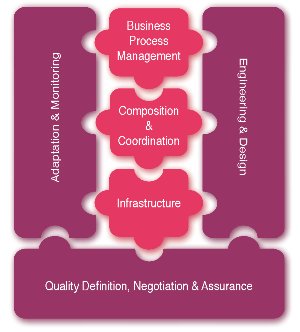
\includegraphics[width=.3\textwidth]{part1/pics/scube-overview.png}
  \caption{S-Cube Research Framework}
  \label{fig:scube-overview}
 \vspace{-0.4cm}  
\end{wrapfigure}
Cette thèse a été menée dans le cadre du Réseau d'Excellence Européen S-Cube.
S-Cube~\footnote{http://www.s-cube-network.eu/} est un réseau d'excellence Européen en Logiciels, Services et Systèmes. Ce réseau d'excellence a pour ambition de coordonner la recherche européenne sur les services logiciels. En connectant la recherche à l'industrie, et en unifiant des recherches multidisciplinaires, S-Cube cherche à développer des méthodes d'ingénierie des services, agiles et globales, et spécifier les principes et techniques d'adaptation des services.\\
Ce réseau d'excellence a été financé par le programme de recherche Européen (FP7) 'Coordination', sous le thème des Technologies de la Communication et de l'Information (ICT). En plus d'offrir un fort support pour les collaboration et des opportunités de mobilité entre les instituts de recherches Européens, S-Cube a financé plusieurs thèses de doctorat pour les différentes couches de la vue globale présentée en figure~\ref{fig:scube-overview}\\



\subsection{Contribution}


La contribution de cette thèse s'inscrit dans les travaux du groupe de travail 1.2: {\it Adaptation and Monitoring Principles, Techniques and Methodologies for Service-based Systems} de l'activité de recherche collaborative(JRA) 1 : {\it Engineering and Adaptation Methodologies for Service-based Systems}\\

L'objectif général du JRA1 est de "concevoir un ensemble de principes intégrés, de techniques et de méthodologies pour la conception, l'adaptation et la surveillance d'applications basées sur les services, tout en garantissant la qualité du système de bout en bout, et sa conformité au contrat de service", d'après la description du travail d'S-Cube\footnote{DoW Amendment 4, December 6th, 2010}.\\
La contribution de cette thèse comporte un modèle de composant qui: implique de nouvelles méthodes et techniques d'ingénierie, permet l'adaptation d'applications basées sur des services, et offre des moyens de réaliser des vérifications de la conception au déploiement pour assurer la qualité de service.\\

Plus précisément, la contribution de cette thèse s'inscrit dans le groupe de travaille JRA-1.2, qui cherche à définir de nouveaux principes et techniques pour l'adaptation et la surveillance d'applications orientées services, globalement sur l'ensemble des couches. Si \enti{} ne s'intéresse pas à priori aux problématiques de surveillance, il permet de résoudre les questions d'adaptation.\\

Du point de vue du projet S-Cube, \enti{} peut aussi être considéré comme une brique logicielle permettant l'adaptation des couches d'infrastructure ou de composition et coordination de services, couches présentés sur la figure~\ref{fig:scube-overview}. 


\selectlanguage{english}

\part{Context, Requirements and State-of-the-Art Review}
%\setcounter{chapter}{0}

%%  une page de citation (pas indispensable)
%\vspace{12cm}

~\vspace{1cm}
\begin{flushright}
{\it Every person I work with knows something better than me.\\
My job is to listen long enough to find it and use it.}\\
Jack Nichols
\end{flushright}
\vspace{2cm}

The European population is getting older due to a conjunction of two factors. First, the decrease of births reduced the part of youth in the population. The second factor is the soon arrival of post-war "baby-boom" people to the age of retirement. Both of these factors imply a radical change in the age pyramid, and in the socio-economical environment of European countries. A consequence of this ageing of the population is an emergence of needs and requirements to face this global evolution.
\par Over the past few years, home automation technologies have been tending to democratize. More and more technical solutions are proposed to automate shutters, garage doors or lightning in houses. These facilities improved the quality of life of the European population. Now they sound like an interesting tool that could help and offer support to elderly people in their home.\\

As an introduction, chapter~\ref{ch:introduction} presents the Ambient Assisted Living and Home Automation domains, in order to extract some general requirements and outline the contribution of this thesis.\\
After this introduction, a state-of-the-art review in AAL projects, Home Automation, and software engineering approaches is carried out in chapter~\ref{ch:survey}. 
Chapter \ref{ch:summary} ends this first part with a summary of the state of the art, and announces the contribution of this thesis.


\chapter{Introduction}
\label{ch:introduction}


Home Automation and the Ambient Assisted Living(AAL) domains have been of major influence on this work. Home Automation technologies offered a plethora of technical solutions with various constraints, while AAL brought substantial real life material in terms of requirements, needs, or use cases.\\
This introduction chapter presents these domains in sections~\ref{sec:context.aal} and~\ref{sec:context.homeautomation}. This presentation enables section~\ref{ch:requirements} to list some general requirements identified in these domains. Section~\ref{sec:scope} defines the scope of this work before section~\ref{sec:introContrib} outlines the contribution of this thesis.


\section{Ambient Assisted Living}
\label{sec:context.aal}

\begin{wrapfigure}{r}{60mm}
	\vspace{-0.5cm}
  \centering
  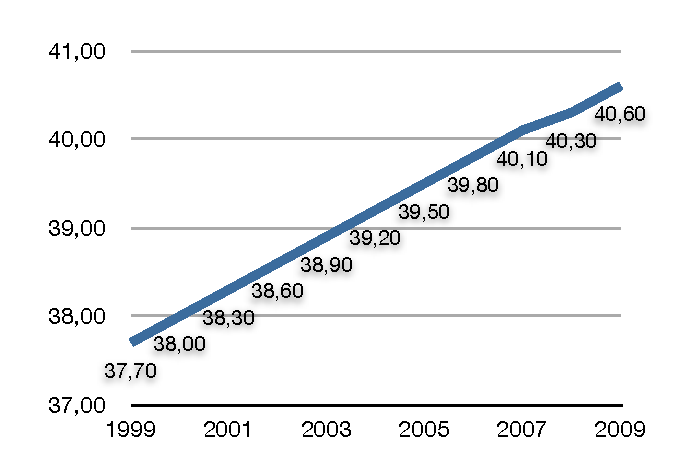
\includegraphics[width=60mm]{part1/pics/medianAgeEUPop.pdf}
  \caption{Median Age of EU Population - Source Eurostat}
    \label{fig:medAge}
	\vspace{-0.5cm}
\end{wrapfigure}

\subsection{The origins}

According to Eurostat~\footnote{http://epp.eurostat.ec.europa.eu/portal/page/portal/eurostat/home}, the median age of European Union (27 countries) population has been growing regularly. From a median age of 37.7 years in 1999, it increased to 40.6 years in 2009 as shown on figure~\ref{fig:medAge}. It is a fact; the European population is getting older each year. This ageing of the population is the result of the combination of several factors, among which are the ageing of baby-boomers, and the decrease of birth rates.\\

The {\bf "Baby Boom"}\\
During the Second World War the birth rate stagnated, resulting in a similar number of births from 1939 to 1945. This stagnation is visible in figure~\ref{fig:agePyramidEU272009}, at the level of people aged between 64 and 70. The "Baby Boom" describes the rapid and strong increase in the number of births that occurred after the Second World War, thus between 1945 and 1968. Actually, 4.9 million people were born in 1944 in the EU, 7.6 million were born in 1968 (+35.8\%). People born during the "Baby Boom" are now (in 2011) 43 to 68 years old, and will soon retire.\\

{\bf Decrease in birth rates}\\
As can be noticed in figure~\ref{fig:agePyramidEU272009}, a decrease in birth rates began at the end of the sixties. From 7.664 million persons born in 1968, the number of births fell to 5.061 million in 2002 (-33.4\%). In \cite{Bosch:1998}, Xavier Bosch explains that this phenomenon is due to a multitude of factors such as an increase in the use of contraception, the raise of the number of single people, or the increase in the percentage of women in the workforce.\\

\begin{wrapfigure}{r}{60mm}
	%\vspace{-0.8cm}
  \centering
  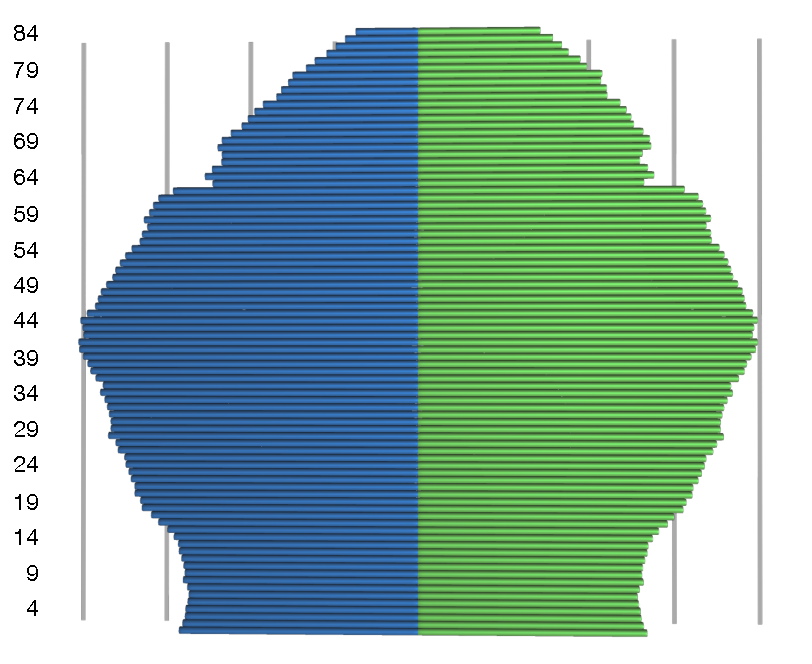
\includegraphics[width=60mm]{part1/pics/AgePyramidEU272009.pdf}
  \vspace{-0.8cm}
  \caption{Age Pyramid EU (27) in 2009. - Blue: M, Green: F - Source Eurostat}
  \label{fig:agePyramidEU272009}
	\vspace{-0.5cm}  
\end{wrapfigure}

Europe will soon have to face the increase in the retired portion of the population, and a simultaneous decrease in young people entering working life. By 2050, the number of people over 65 in the EU will have increased by 70\%, and the number of people over 80 will have grown by 170 \%.\\

In order to be ready on time, governments must address the economic and social implications of an ageing population. They must prepare for increasing demands on healthcare, as a rapidly ageing society heralds growing populations with chronic diseases, disabilities, and increasing health needs.\\

\subsection{The concept}
\label{subsec:aalConcepts}

The Ambient Assisted Living Joint Programme~\cite{jointAALProgram} defines the concept of \gls{aal} through 6 dimensions.\\
{\bf Autonomy} By increasing the autonomy, the self-confidence and the mobility of elderly people, \gls{aal} tends to extend the length of time people can live in their preferred environment. \\
{\bf Activities} Maintaining physical or intellectual exercise helps elderly people to remain in good health, and prevents a decrease in capacities.\\
{\bf Assisting} individuals at risk, by promoting a better and healthier lifestyle.\\
{\bf Securing} support and maintaining the network around the individual, including family, friends and social activities, to enhance security and prevent social isolation.\\
{\bf Supporting} carers, families and care organizations in their everyday activities.\\
{\bf Streamlining} the use of resources dedicated to elderly people, by increasing their efficiency and productivity.\\

There are many solutions to address these dimensions. Automation of some tasks can enforce autonomy, and the use of mechanical aids can improve mobility. Social workers and health professionals can propose activities, support and assistance. Unfortunately, healthcare associations or companies have difficulty in hiring people for these jobs. Indeed, qualified people are not numerous enough, and financial constraints are strong in this domain.\\
~\vspace{0.5cm}

A solution, in assisting both helped people and helpers, could be to use Home Automation technologies in conjunction with ICTs and human interventions. Section \ref{sec:context.homeautomation} presents this domain.



\section{Home Automation}
\label{sec:context.homeautomation}

%\begin{wrapfigure}{r}{40mm}
%	\vspace{-0.5cm}
%  \centering
%  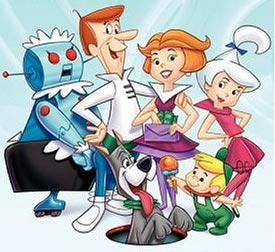
\includegraphics[width=40mm]{part1/pics/Jetsons.jpeg}
%  \caption{The Jetsons}
%	\vspace{-0.5cm}  
%\end{wrapfigure}

In 1962, William Hanna and Joseph Barbera created the Jetsons cartoon family. In this carton, George and Jane were living in the \textit{Skypad Apartments} in \textit{Orbit City} with their children Judy and Elroy. Their housekeeping robot, Rose, handled all chores not done by the numerous automated appliances triggered with some push-buttons. Apart from the fact that it is just a fiction cartoon, it describes well the idea of smart homes or home automation. Let us get into a bit more detail about home automation, and see why it is still not applied in everyone's home.


\subsection{Application domains}
Home automation has for too long been perceived as it was presented in the Jetsons: a set of costly, useless, funny pieces of technology.\\
Obviously, personal home theaters, multi-room media systems, smart colored lighting controllers will always exist and make a good showcase of what is possible. Besides, the use of more utility-oriented home automation is soaring. Home or building automation technologies, among others, ease the management of lighting control, shutter control, heating, ventilation, air conditioning, energy management, metering, monitoring, alarm/intrusion systems, household appliances, audio/video and lots more. However, people are not ready to pay for the automation of tasks they can execute by themselves.\\
Widely used in industry buildings and plants, the automation of the lighting or heating systems has brought substantial savings of energy and money. This industrial experience makes it possible to imagine the benefits of installing such systems in homes. The minimization of power consumption with a maximization of welfare is acceptable, even dreamed of by everybody.
By extension, alarm systems, automatic garage doors and shutters can also be managed this way, rendering a global and coherent service to inhabitants. 

\subsection{Technologies}

The devices encountered in home automation originate from different business domains. M. Nagy says in~\cite{Terziyan:2009} that "A major problem is inherent heterogeneity [...] with respect to nature of components, standards, data formats, protocols, [...]". Indeed, it can be a problem from many aspects, but it is also a set of tools waiting to be connected.\\

{\bf Communication Media}\\
Four main communication media can be differentiated in home automation technologies: the {\it Bus}, the {\it Radio}, the {\it \gls{plc}} and {\it Infrared}.
Devices use these communication media to communicate with each other, and offer a technical functionality.
The choice of a medium is linked to the constraints to be addressed. For instance, a Bus link is highly reliable, but requires the wiring of the entire house. On the other hand, Radio communications do not need any additional wiring, but are less reliable and batteries have to be changed regularly.\\

{\bf Plethora of protocols}\\
Historically, there is no specific home automation brand or manufacturer. It all comes from different trades such as electricity or \gls{hvac} control. According to the specific needs of their domains, each home automation manufacturer has developed a specific communication protocol for its devices to operate with each other. They also use several communication media to carry the communications. A consequence of that is the huge number of devices, protocols and media available on the home automation market, illustrated in section~\ref{subsection:homeAutomationDetails}. 
Technical solutions proposed by the Home Automation domain are so numerous, that there may be a solution for each need, in almost each domain. Nevertheless, due to this great diversification, no common management tool exists so far, resulting in expensive mono-manufacturer closed solutions, or no solution at all.\\
Even if home automation technologies have existed for many years, no real standard has been released. Imposing a global standard, as was the case for the IP protocol for example, seems to be the best way to address such an issue. Naturally, each domain has created its communication protocol adapted to each business concern. Thus, finding a common protocol, used and understood by all devices from all domains, appears to be a very difficult task. And even if one finally emerges, developers will still have to deal with legacy devices using proprietary protocols.\\
Moreover, the old way manufacturers think adds to the complexity of the problem. They still think that a closed world (I mean non-public protocol specifications) is a world that can be controlled. Indeed, it is true, but it is also a world that fewer and fewer people want to enter, because they are afraid of the captivity imposed by such solutions. Captive systems are often well tested, because of the  restricted number of available devices, but there is also a risk for these components of being removed from the market one day. In these conditions, people could not replace these components with compatible others, and are thus really concerned with the sustainability of the adopted solution.\\



\section{Identification of requirements}
\label{ch:requirements}

The domain of Home Automation requires a new breed of technology to easily manage installations and answer specific needs. The lack of such a tool, able to operate any home automation technology and create solutions for specific needs of elderly people, makes the adoption and use of these technologies marginal. This absence of a tool may be due to the complexity and number of requirements inherent to home automation systems. This section aims to identify a set of required properties for a software tool to be adopted by manufacturers, installers and users.\\

The requirements presented in this section had been identified in \cite{Nain09a}. This section completes the list and elaborates on them.\\


%\subsection{Required properties}

{\bf Interoperability}\\
Interoperability is described as the ability for systems to operate with each other. Even if 'system' is quite a generic word and encompasses lots of things, the idea behind interoperability is simple. Given two or more systems, how can one ensure that each of them is operable with another one? For instance, if I have a light management system and another one for shutters, how can I guarantee that systems will be able to communicate in order to be of use for the user?\\
A closed environment, in which all devices come from the same manufacturer, avoids the problem. A communication interface, common to all components, also deals with the issue.
Interoperability becomes a complex problem when the environment is open and when several technical concerns have to be handled in a single place (lighting and heating management for instance).\\
In the context of \gls{aal}, each solution will be uniquely deployed, because each patient, each helped person has specific needs due to his environment or illness. Indeed, specialists in this domain will select different technical artifacts or services, according to each person's needs. Those solutions will have to cooperate with each other in a single system, to perfectly meet the user's needs, whoever their manufacturer or whatever their communication protocol may be.\\


{\bf Openness}\\
Openness means making all offered functionalities available for third party applications, or different uses other than the one initially imagined. 
In closed systems, customers are limited to the functionalities and evolutions proposed by the solution's manufacturer. If the system deployed was built specifically for a customer, any evolution is very costly. Keeping the system open to external contributions may reduce the number of demands for costly system modifications or add-ons. In any case, it is also an open door for new unforeseen appliances adding smart behavior to a reliable set of functionalities.\\
This is a clear challenge in computer sciences, and in general when considering communications and interactions between objects or systems. 
The definition of a home-made interface fulfilling the requirements is easier than fitting into a good practice or a standard that does "almost what we want but not completely".\\
Openness is a strong requirement in home automation systems, as it has been in computers. Today, a computer manufacturer would not create a specific connection port, compatible with no other computer, unless he wants to create a new captive market.\\

{\bf Adaptation}\\
In a perfect world, devices never fail, services are always available and the Internet is always available. As demonstrated every day, the world we are living in is not perfect. Software systems, or systems dealing with objects or services linked to everyday life actions, have to take their execution environments into consideration. They should be able to dynamically adapt to changes around them while they are running, in order to maintain a given level of services or functionality as long as possible. Obviously, these adaptations should not require any reboot of the system, because a reboot could make all in-house functionalities unavailable. Lastly, an adaptation is not intended to add or remove any system functionality permanently. Otherwise, it is an evolution.\\
Execution policies or system reactions must be easily modifiable, in order to take into account any change in the user's requirements. For instance, depending on the level of dependency of an elderly person, the system may completely, partially or not at all automate the management of certain household functions such as heating or shutter management. This type of change in system behavior has to be made simple and operable by any authorized person, even with no specific skill in this domain.\\
Most of all, these changes during runtime must not affect the execution of basic security functions (such as emergency call handling), neither in their behavior, nor in their execution during adaptation.\\
Adaptations do not only concern technical elements, but also the user himself. All users are different. While some may be interested in new technologies, others are completely agnostic. When some are able to remember and learn how the system behaves, others may experience some memory loss. Where some have vision disorders, others experience hearing limitations. Software systems should be able to take into account these disabilities and adapt to their evolutions and to users' requirements.\\

{\bf Evolution}\\
Evolution in the context of home automation and/or assisted living is a key requirement. Needs or uses are changing, protocols and technologies also. Some functionalities may finally be required, whereas others can become useless and need to be uninstalled. Security or communication protocols can be improved and deployed in new versions that have to be taken into account without needing to re-implement the entire system.\\
Moreover, systems deployed in a house or a building, in charge of its management and the comfort of its inhabitants, have to be designed to serve during the entire lifetime of the building (even if hardware changes may be required). Therefore, they must be ready to accommodate future and unforeseen evolutions such as the installation of new services/functionalities for example.\\

{\bf Variability Management}\\
No house or building is like any other. This is because of structural or ground specificities, because of a particular user's need or just because no one would like to have exactly the same house as his neighbor. Thus, each installation will have specific devices deployed, using specific versions of protocols, and providing several functionalities. The development, by hand, of a specific control system for each installation is completely out of the question. It would be too costly and error prone. A global management tool should exist to deal with the inherent variability of such systems.\\
People responsible for designing a solution for an installation query should have some tools at their disposal to help them in choosing devices to install, or to assist them in selecting devices from all the catalogs of all manufacturers.\\

{\bf Remote Control}\\
More and more, people want to remotely access their belongings. This is also true for their homes. They would like to be able to remotely check the lights status, run a bath or switch on the alarm system that they forgot.\\
In the context of building management facilities, specialized companies have different solutions to check the state of a building system. They either have remote access to all systems, or they check locally by hand. Obviously, the local solution is longer viable in the context of our society. Systems deployed to control buildings or homes should have remote access possibilities (under access control and agreement) to allow for remote diagnosis, corrections, or evolution actions from a control center.\\

{\bf Distribution}\\
Today's systems work more and more with or on different execution platforms, and communicate more with each other. This is particularly true for home automation. For redundancy reasons and service level insurance a building and even a house can be equipped with multiple, independent, but connected controllers. These controllers can share the different functions to balance the loads on platforms, or offer a connection to a specific, locally-connected device. When a running platform fails, other platforms aware of its job can stand in temporarily, until the original controller is back in operation. Also, devices are becoming smarter and may make decisions by themselves. As a consequence, decisions and control could be distributed to several smart pieces of equipment.\\

{\bf Safety \& Security}\\
As presented in the context of this work, safety and security are very important requirements for home automation systems. Indeed, they themselves have to be safe and secured to be able to play their role in difficult situations and improve the security and safety of people and goods.
A minimum service level has to be guaranteed, for inhabitants not to remain stuck in the house in the case of an emergency. Moreover, the access policies of the system have to be sufficient to avoid unauthorized access, and simple enough not to become a constraint for authorized carers.\\
Several tools such as simulators, tests, or model checking, can be used to check and improve the reliability and the safety of such systems.\\

{\bf Acceptability \& Accessibility}\\
In the domain of home automation, deployed solutions, whatever their nature, have to take into consideration interactions with all inhabitants. Whether they are children, teenagers, young workers, parents, retired or old people, all of them must be able to interact with the system. 
Checks have to be performed on all solutions proposed, to ensure all users can control, or obtain information from the system and keep control.\\

New requirements for software are emerging from the accessibility of home automation technologies. The evolution of the software during the building's lifetime, its adaptation to cope with changes in its execution environment and the huge variability of technologies and protocols to be guaranteed to inter-operate, are triggering new challenges for software engineering.

\section{Scope of this work}
\label{sec:scope}
The list of requirements presented in the previous section could be completed. A particular situation can bring many other issues for software engineering.\\
This thesis focuses only on a subpart of these requirements and aims to propose a solution to conjunctively address interoperability, adaptation, openness, evolution, variability management and, partially, safety and security issues. The first goal of this thesis was to end up with a working solution able to cope with this sub-list of requirements. Other ones will be addressed in future works. As for safety and security issues, the work realized in this thesis partially addresses the problem, since questions about privacy and information security concerns have been decided as out of scope. The focus was more about ensuring consistency of assemblies and a fail-safe system.

\newpage
\section{Contribution of this thesis}
\label{sec:introContrib}

Software can no longer be built on a once-off basis. Customizable, reliable and personalized solutions have to be deployed in the short terms to meet changes in users' needs or in the environment at any time. Moreover, the specificities of each installation make it very hard to create a unique piece of software able to cope with all technologies, concerns (such as energy consumption) or unpredictable evolutions.\\

In the electronics domain, the number of components and their always-possible connectivity have offered technicians and engineers the means to create various solutions. Even many years after their assembly, electronic devices can still be repaired or completed with new features. The proposal made in this thesis is to take advantage of the electronic way of doing to improve the flexibility of software systems while keeping a high level of safety and security.\\
To this end, the contribution of this thesis can be described from three aspects:
\par - A constraint-relaxed component model that leverages the software flexibility, by offering ways to connect any component to any other. This aspect addresses interoperability issues and evolution requirements
\par - Modeling tools to create, modify and simulate component assemblies, check their consistency and validity before their (re-)deployment at runtime. Safety and security, as much as variability management are requirements covered by this aspect of the contribution.
\par - An execution environment built over a service-oriented runtime, to support the proposed component model and cope with adaptation and evolution requirements at runtime.\\


\chapter{State-of-the-Art Review}
\label{ch:survey}

The review proposed in this chapter is made if three sections.\\
Section~\ref{sec:background} starts with a description of the Ambient Assisted Living domain from which social requirements have emerged, and it presents some projects on this topic. It then introduces some home automation technologies, their use and goals in several projects. The overview of these two domains makes it possible to sense more precisely the needs for a new breed of software for these domains.\\
Section~\ref{sec:generalPurposeApproaches} then presents several general purpose software approaches and tools that have been considered for the resolution of the problem targeted. Each of them is evaluated against the requirements identified in the introduction. However, general purpose approaches seem not to be specialized enough to meet the requirements of the \gls{aal} and home automation domains.\\
For this reason, section~\ref{sec:domainSpecificApproaches} evaluates some selected domain-specific approaches with respect to the same requirements as for general purpose ones.\\
Finally, the review made in this chapter is summarized in chapter~\ref{ch:summary} which uses this basis to specify the contribution of this thesis.


\section{Background on AAL and Home Automation}
\label{sec:background}

Ambient Assisted Living is a hot topic in Europe. Several projects have been led to address different aspects and try to cover the needs inherent to a home-keeping situation. This section introduces some of them.

\subsection{Projects in AAL}

The \glsreset{aal}\gls{aal} Joint Programme~\footnote{http://www.aal-europe.eu} is a collaborative association of twenty European Union Member States, plus three Associated States. They group together the AAL Association, whose main objective is to enhance the quality of life of elderly people, through the use of \gls{ict}. Their main activity is to found R\&D projects in the \gls{aal} domain and to publish annual calls for project proposals.\\
The total budget planned for the \gls{aal} Joint Programme is €700 million, half of which is to be funded by public resources (AAL Partners plus the European Commission) and the other half by private participating organizations. According to the 13\up{th} article of the EC decisions 743/2008/EC~\cite{743/2008/EC}, funding from the European Commission is taken from the budget allocated to the \gls{ict} theme of 'Cooperation' under the FP7 Specific Programme of the same name. Thus, the \gls{aal}-JP is set to last from 2008 to 2013, to correspond to the FP7 dates.\\


The {\bf ASK-IT} project~\footnote{http://www.ask-it.org/ (march 2011)} ran from 2004 to 2008, and aimed at providing {\it Ambient Intelligence} to support and promote the mobility of impaired people~\cite{Wiethoff:2007}. It laid to the development of a software framework, and a set of tools for mobility. Among other things, a {\it Domestic Module} has been created to support the provision of seamless home environment management, to the mobility-impaired traveler on the move.\\

In a slightly similar approach, the {\bf SOPRANO} project~\footnote{http://www.soprano-ip.org/ (march 2011)} intends to design an \gls{ict} system to foster the comfort and safety of elderly people in their everyday life. In this project, a strong effort is made to measure the acceptability of the solutions.
SOPRANO~\cite{Sixsmith:2010} aims to maximize the acceptability of the services, especially in populations vulnerable to loss of independent living. This is achieved by ensuring control of the environment by users, where they so wish and by using extended user-centered design techniques.\\

{\bf INHOME IST} Project~\footnote{http://cordis.europa.eu/fetch?ACTION=D\&CALLER=PROJ\_IST\&RCN=80489 (march 2011)} is also an interesting project in this context. Completed in December 2008, its goal was to enhance the autonomy and the safety of elderly people at home~\cite{Vergados:2008}. It led to the development of a set of services such as activity monitoring, home environment management, task scheduling, flexible AV stream handling, and hence, flexible access to  household appliances.\\

As for, the {\bf GUIDE} project~\footnote{http://www.guide-project.eu/ (march 2011)}, it endeavors to provide a framework~\cite{Ciccarese:2005}, a user model toolbox and a handbook, along with graphical user interface components, in order to ease the creation of graphical user interfaces answering the special needs of elderly people.\\

All these projects try to improve the comfort, safety and security of elderly people by means of technical aids.
Home Automation is a vast field that offers many solutions to ease or help in the realization of everyday tasks that can become difficult with ageing. Basic elements of this domain have been introduced in section~\ref{sec:context.homeautomation}.

\subsection{European research}
The European 'Cooperation' Programme of the FP7 is quite a good representation of European countries' current concerns and research themes. According to the FP7 factsheet\cite{fp7-factsheets}, €32.365 million are allocated to different themes. The major theme, which is allocated 28.72\% of the FP7 'Cooperation' funds, is \gls{ict}. In second position with 19.07\% comes the health theme. Third and fourth positions are Transport and Nano-Productions respectively, with 13.18\% and 11.03\%, followed by the Energy and Environment themes consuming 7.25\% and 5.67\% of the overall budget.\\
Thus, three of the top five concerns of Europe are \gls{ict}, Health, and Energy and the Environment (assuming Energy and the Environment can be grouped as a unique theme).\\

Using \gls{ict} to improve the quality of life of people is an idea that can be identified in the background of several projects throughout the world. Section~\ref{sec:homeautomation.projects} presents some of them with a focus on those using home automation technologies.

\subsection{Home automation in projects}
\label{sec:homeautomation.projects}

Information reported in this section has been partly collected from a talk by Luc BALANGER, director of the Communication Networks department at FFIE (French professional association of electrical engineering companies).\\

{\bf Asian} countries have developed strong market sensitivity to video games. Some TV channels are even specialized in the live transmission of gaming parties, involving professional and sponsored gamers. Over the past few years, several studies and news programs have reported a kind of addiction of a portion of the  population to video games. In particular, A. Faiola in~\cite{Faiola:2006} states that about 2.4\% of 9 to 39 year-old South Koreans are believed to be suffering from game addiction, according to a government-funded survey. Another 10,2\% of them were found to be obsessed with playing electronic games.\\
Some home automation manufacturers are working on products to make the game more real. The goal is to give gamers the sensation of being in the game, and playing as a first person, using for instance 7.1 speaker systems or 3D visualization devices. This aspect of home automation is clearly entertainment oriented.\\

{\bf The United States} is also concerned by video game addiction of youth. However, home automation does not target this domain, but a much more prominent one in the US. The safety and security of people and goods has been a huge market in the United States since the 9-11 events, as explained by Terrell E. Arnold, a retired Senior Foreign Service Officer of the United States Department of State in~\cite{Arnold:2011}. Also called the "fear" market, American people are investing a lot of money to feel safe. In this field, video security cameras can be deployed in homes, for inhabitants to be able to remotely see what is happening. Presence simulation is a must in this kind of systems, feigning somebody's presence in the home by automatically switching on and off lights when inhabitants are away.\\

In {\bf Japan}, safety and security are also two important requirements and necessities, but not for the same reasons. As recently demonstrated, nature is not kind in Japan. Volcano, earthquakes and tsunamis are real dangers. The JEITA House Project~\footnote{http://www.eclipse-jp.com/jeita} made it possible to automatically secure the house when an earthquake is detected. For instance, the solenoid valve controlling the arrival of gas in the house is switched off when an alert is received. This security has been enabled by the use of home devices able to communicate with each other, or with the centralized house manager. The JETI project also had an orientation toward improving the comfort of people. Asian people are fond of multifunction toilets or showers, and more generally, pay a strong attention to their well-being and health. A centralized house manager can improve the well-being of inhabitants by making everyday devices smarter. Manufacturers in this domain design their products to be more and more connected, and full of high-technology features. Moreover, each device is given a specific address making it possible to remotely control almost everything in the house. For example, it is possible to remotely run a bath using a smart phone for it to be ready when the resident is back home.\\

Home automation has a bad reputation, due to several advertisements that promoted useless functions. It thus has been considered as a costly, useless technology, for people fond of high technologies. Nevertheless, home automation technologies have quietly grown, and are today very rich in terms of communications, functionalities and uses.


\subsection{Home Automation details}
\label{subsection:homeAutomationDetails}

The evolution of concerns and needs in the home automation domain has led manufacturers to adapt their products over the years. As a consequence, lots of products communicating through many different media are available today. According to their manufacturers, and to their domains of use, devices also come with their own transportation protocols making their diversity even greater. This section briefly presents a non-exhaustive list of protocols and media used by home automation products to highlight the complexity of this domain with relation to the huge variability of solutions.\\

%~\vspace{0.5cm}
\subsubsection{Communication Media}

{\bf Communication Bus} The bus is physically a wire, a link between devices responsible for transporting data packets from a source to a destination. When a data packet is sent, every device connected to the bus receives the packet. Most of the time, devices ignore the packets, unless the destination address of the packet is the device's address. Ethernet is probably the most famous ambassador of this communication medium.\\

{\bf \gls{plc}} is a special kind of bus. The main idea of this communication medium is to reuse existing cable infrastructure to avoid adding a new specific communication cable. As the most common cable present in all houses is the power line, this technology injects data into the power line by modulating in a carrier wave. All transceivers plugged into the line can then decode the data from the carrier wave modulations.
This communication medium tends to be more and more used, as it offers great data transfer rates and does not impose any new wiring.\\

{\bf Radio} The radio medium is widely used, thanks to its wireless property. Radio devices are quite complicated to design, because of the trade off between energy consumption and protocol reliability. However their deployment is easy, and does not require a major work.
Many manufacturers use the free ISM radio band. As a consequence, the ISM frequencies are noisy, and protocols have to secure their communications.\\

{\bf Infrared} The infrared communication medium is employed for specific appliances. Indeed, there can be a lot of noise coming from the natural light disturbing the receivers. Since this medium is based on an optical link (using infra-red), both transmitter and receiver have to face each other. This is a strong limitation that makes the use of this medium difficult in home automation. In fact, devices are rarely facing each other.
Nevertheless, it still is a good medium for a human-computer interface such as a remote control. Users can give orders to the system using a remote control, thanks to receivers disposed in many places around the house.\\

{\bf Links between media} It is sometimes necessary to use a combination of different media to cover requirements from both the users and the infrastructure of the solution. As a consequence, manufacturers have developed families of devices, which use several communication media. Obviously, they also created products to transfer orders/communication frames from one media to another, so that all their products can obtain the information.\\

\subsubsection{Transport Protocols}

{\bf io-homecontrol\up{\textregistered}} is a two-way radio technology and a proprietary protocol. Organized in an association, a dozen of industrial manufacturers provide products compatible with io-homecontrol. Partners of this association are Honeywell, Niko, Somfy, Velux, Groupe Atlantic, Assa Abloy, Ciat, Renson, WindowMaster, SecuYou and Overkiz. This technology is embedded in house equipment such as roof windows, vertical windows, roller shutters, gates, garage doors, front doors, alarm systems, lighting, ventilation, heating systems, etc. A single control can monitor and pilot all the io-homecontrol compatible equipment in the house.\\
%This consortium is closed and not interested by external collaborations with public R\&D centers, or schools.\\

{\bf IOBL} In One By Legrand is a proprietary protocol used by Legrand (a French electrical component manufacturer). Legrand offers many devices able to interact with each other. These devices control lights, shutters, or heating systems. Being proprietary, no other device manufacturer offers compatible products. IOBL products are able to send and receive orders from infrared medium or \gls{plc}.\\

{\bf X2D} Delta Dore is historically a French heating system manufacturer. This company has extended its activities to home automation and alarm systems, for home and building control. For their products to communicate, they have developed a communication protocol called X2D, using radio, bus and PLC media. Just as IOBL, the protocol is private, and no other manufacturer offer compatible products.\\

{\bf X10} is a communication protocol for low cost home automation products. Sensors and actuators send data frames over \gls{plc} or radio to a maximum of 256 addresses, with no acknowledgement. It is thus impossible to know if an order has reached its destination, and there can be only one order at a time on the network.\\
This protocol is quite limiting in term of number of devices, and guarantee of service, but it works and is pretty cheap compared to other product families. Moreover, technical specifications are available.\\

{\bf Z-Wave} is a wireless technology to remotely control home appliances, entertainment products, and access systems, running in the 868MHz ISM band. Grouped into the Z-Wave Alliance\footnote{http://www.z-wavealliance.org/}, 160 manufacturers offer interoperable products in these domains, using this closed protocol. Based on a mesh topology, Z-Wave data frames can transit through several devices around the house to reach their destination. This is an interesting faculty to overpass radio obstacles and ensure delivery.\\
 
{\bf ZigBee} is an open standard addressing low-cost, low-power M2M wireless networks. It was released by the IEEE in 2003 and over 300 manufacturers have since then joined the ZigBee Alliance. Working on 2.4GHz, 900MHz and 868MHz, ZigBee has been designed to be able to work in hostile radio environments. Network topology can be point-to-point, infrastructure or mesh, and accepts up to 65,000 nodes. Wireless products compatible with the ZibBee specifications target remote control, home automation or sensing domains.\\

{\bf 6LoWPAN} is the name of a working group at the Internet Engineering Task Force (IETF). This group aim to reduce the memory footprint of IP frames (and principally IPV6 frames) for the protocol to be used in devices and networks with low power availability. This protocol would make it possible to use the powerful IP routing mechanisms, in sensor networks or distributed embedded applications, making them operable from any classical IP network. Specifications of 6LoWPAN can be found as RFC 4944\footnote{http://tools.ietf.org/html/rfc4944} and RFC 4919\footnote{http://tools.ietf.org/html/rfc4919}.\\

{\bf European Eib/KNX consortium} The KNX Association\footnote{http://www.knx.org} was founded in May 1999, by the members of the EIBA (European Installation Bus Association), EHSA (European Home Systems Association) and BCI (BatiBUS Club International) associations. Its mission is to develop and promote the KNX standard so that it is recognized as "The worldwide standard for home and building control". The KNX standard has been designed to enable the control of applications in industrial, commercial and residential buildings worldwide.\\
KNX has been approved as a European Standard (CENELEC EN 50090 and CEN EN 13321-1), an International Standard (ISO/IEC 14543-3), a Chinese Standard (GB/Z 20965) and a US Standard (ANSI/ASHRAE 135). It groups about 7000 KNX certified products from 200 member companies, installed by more than 30,000 KNX partner installers in 100 countries.\\
KNX is designed to automate and control lights, shutters and heating systems in homes and buildings.\\

{\bf LonMark Intl.} Echelon Corporation\footnote{http://www.echelon.com} is an international company that targets a worldwide transformation of the electricity grid into a smart grid. To achieve this task, Echelon developed LonWorks, a family of products able to interact with each other using the LonTalk protocol. The promotion of LonWorks products to end-users, manufacturers and integrators is ensured by the LonMark Intl.\footnote{http://www.lonmark.org} organization. This organization is also responsible for giving guidelines and help to manufacturers, integrators and end-users to build or simply use LonMark certified products. Lastly, its role is to ensure the interoperability of all products, by verifying that each of them meets the LonMark guidelines to operate on a LonWorks network. The LonTalk protocol designed by Echelon is currently recognized as an international standard (ISO/IEC 14908), a European standard (EN14908) and a Chinese standard (GB/Z 20177.1-2006). In February 2009, over 700 organizations joined LonMark.\\
LonWorks products are mainly used for technical building management concerning lights and HVAC (Heating, Ventilation and Air Conditioning).\\

{\bf BACnet} Developed under the auspices of the American Society of Heating, Refrigerating and Air-Conditioning Engineers (ASHRAE), BACnet\footnote{http://www.bacnet.org} is a Data Communication Protocol for Building Automation and Control Networks. It has been released as an American national standard, a European standard, a national standard in more than 30 countries and an ISO global standard. The protocol is supported and maintained by ASHRAE Standing Standard Project Committee 135, divided into 13 working groups. These groups work to integrate issues from various building aspects from "Objects and Services" cooperation to elevator or lighting management. In February 25, 2011, 503 Vendor IDs were issued from all over the world.\\

\subsubsection{Application Protocols}

{\bf Universal Plug \& Play(UPnP)}\\
\gls{upnp}~\footnote{http://www.upnp.org} is an application level protocol which aims to ease the connection and use of electronic devices, based on a discovery-search mechanism. As a UPnP-Device joins the \gls{upnp} network, it sends an XML description file to all UPnP Control Points. This description provides other devices on the \gls{upnp} network with information such as manufacturer, device type, device model or the unique identifier of the device (UUID). The services offered by a UPnP device are also specified in its description. Each service conforms to a type, a set of UPnP actions that the service renders. Providing such information to other devices on the network makes it possible to use the functionalities of the device without having to install anything (thanks to the standardization of the descriptions and method call mechanisms).\\

{\bf \gls{dpws}}\\
\gls{dpws}~\cite{DPWS} could be considered as a next generation \gls{upnp}. If the goals are the same, DPWS uses WebServices as a transportation mechanism whereas \gls{upnp} uses simple XML over IP. \gls{dpws} is still based on the concept of \textit{services}, \textit{devices}, \textit{operations} and \textit{parameters}. It includes numerous extension points, allowing for seamless integration of device-provided services in enterprise-wide application scenarios.\\


{\bf SIP}\\
\gls{sip} is a protocol for initiating, modifying, and terminating an interactive user session that involves multimedia elements such as video, voice, instant messaging, online games and virtual reality. Developed by the IETF MUSIC Working Group, it was initially published in 1996 as RFC 2543 and updated by the RFC 3261 in 2002.
SIP aims to ease the establishment of communications between multimedia devices using two protocols: RTP/RTCP and SDP.
When RTP is used to transport voice data in real time (the same as H.323 protocol), the SDP protocol is used to negotiate the participant capabilities, codification type, etc.
SIP has been designed in conformance with the Internet model and all the logic is stored in end devices (except the routing of SIP messages).\\
SIP can establish sessions for features such as audio/videoconferencing, interactive gaming, or home appliances over IP networks. It is based on requesting and answering messages and can reuse many concepts from previous standards such as HTTP and SMTP.\\


{\bf XMPP}\\
The Extensible Messaging and Presence Protocol (XMPP)\footnote{http://xmpp.org/ (May 2011)} is a protocol for real-time communication such as instant messaging, voice and video calls, collaboration or lightweight middleware communications.
The core technology of XMPP was invented by Jeremie Miller in 1998 and formalized by the IETF in 2002 and 2003 in RFCs. The latest RFC reviews for XMPP are RFC 6120, 6121 and 6122 published in 2011. The XMPP community continues to define various XMPP extensions through an open standards process run by the XMPP Standards Foundation. An active community of open-source and commercial developers produces a wide variety of XMPP-based software.\\

The complexity of the home automation domain clearly appears from this presentation. Taken individually, each product, transportation protocol, or medium is quite easy to handle. The complexity is due to the huge number of possible solutions for a given problem and to the difficulty of becoming aware of all the benefits and drawbacks offered by each solution.\\
Home automation can be used in various contexts, such as assisted living or energy saving. Professionals in these domains are not aware of the possibilities offered by home automation technologies and home automation engineers are not familiar with each domain's problems.\\
Tools are required to simplify variability management and conciliate home automation technologies with domain-specific problems to bring new solutions.


\newpage
\section{General purpose approaches}
\label{sec:generalPurposeApproaches}

The ageing of the European population and the complexity of home automation technologies require a software tool, able to ease the creation of user-specific, installation-specific software, using home automation devices to provide a personalized service.\\
The development of this tool should rely on an approach adapted to the problem we are trying to resolve here. This section surveys several general purpose approaches and tools, to evaluate their position in relation to our requirements.\\

The survey starts with an overview of Internet of * concepts together with service-oriented architectures. Afterwards, this section presents tools and approaches from the component-base engineering field. This presentation ends with approaches that conciliate services and components; namely component-base architectures for service-oriented applications. Each of these three parts is organized the same way: it firstly describes the general idea of the approach and then details some tools implementing the approach.


\subsection{(Web)Service-Oriented Architectures}
\label{sec:web-services}


\subsubsection{Internet Of * and the Cloud}
\label{subsec:internet_of_stars}

The Internet we know aims at sharing information and facilitating interactions and communications between people or computers.\\

In an article~\cite{Domingue:2009} extracted from the book "Towards the future of Internet", Domingue et al. reports a chart from the web site ProgrammableWeb.com, presenting the number of available APIs (services offered through the web) in fifteen categories. These numbers extracted in November 2008 are reproduced in the chart presented in figure~\ref{fig:api:2008}. Just next to this figure, another chart (fig~\ref{fig:api:2011}) presents the current numbers from the same web site, for the same categories, but three years later. If the repartition has not significantly evolved, the total number of available APIs considerably grown form 612 in 2008 to 2589 in 2011 (plus 423\%).\\
With the evolution of Internet technologies, the services offered through Internet are getting more and more numerous and rich.\\

\begin{figure}
\begin{center}
\subfloat[APIs, 2008]{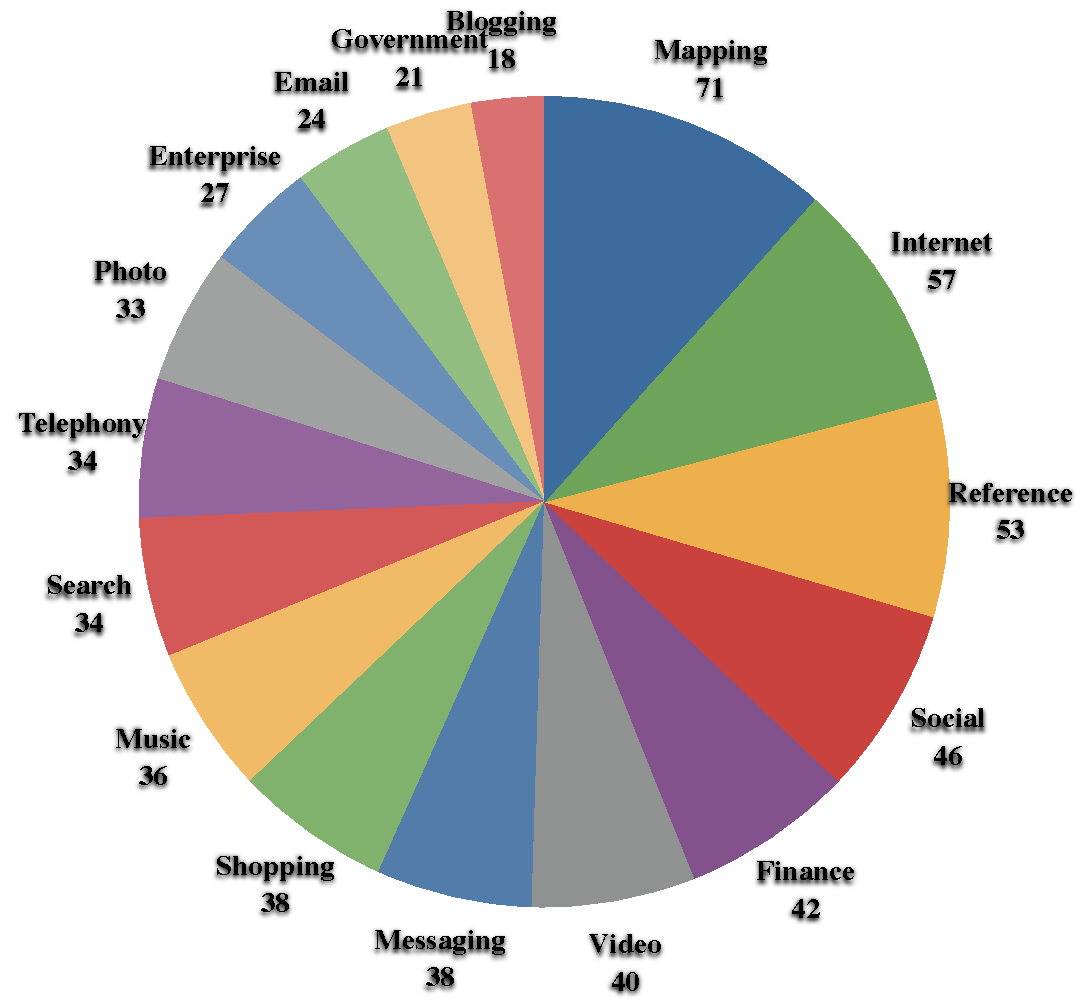
\includegraphics[width=.45\textwidth]{part1/pics/apis2008}\label{fig:api:2008}}
\hspace{3mm}
\subfloat[APIs, 2011]{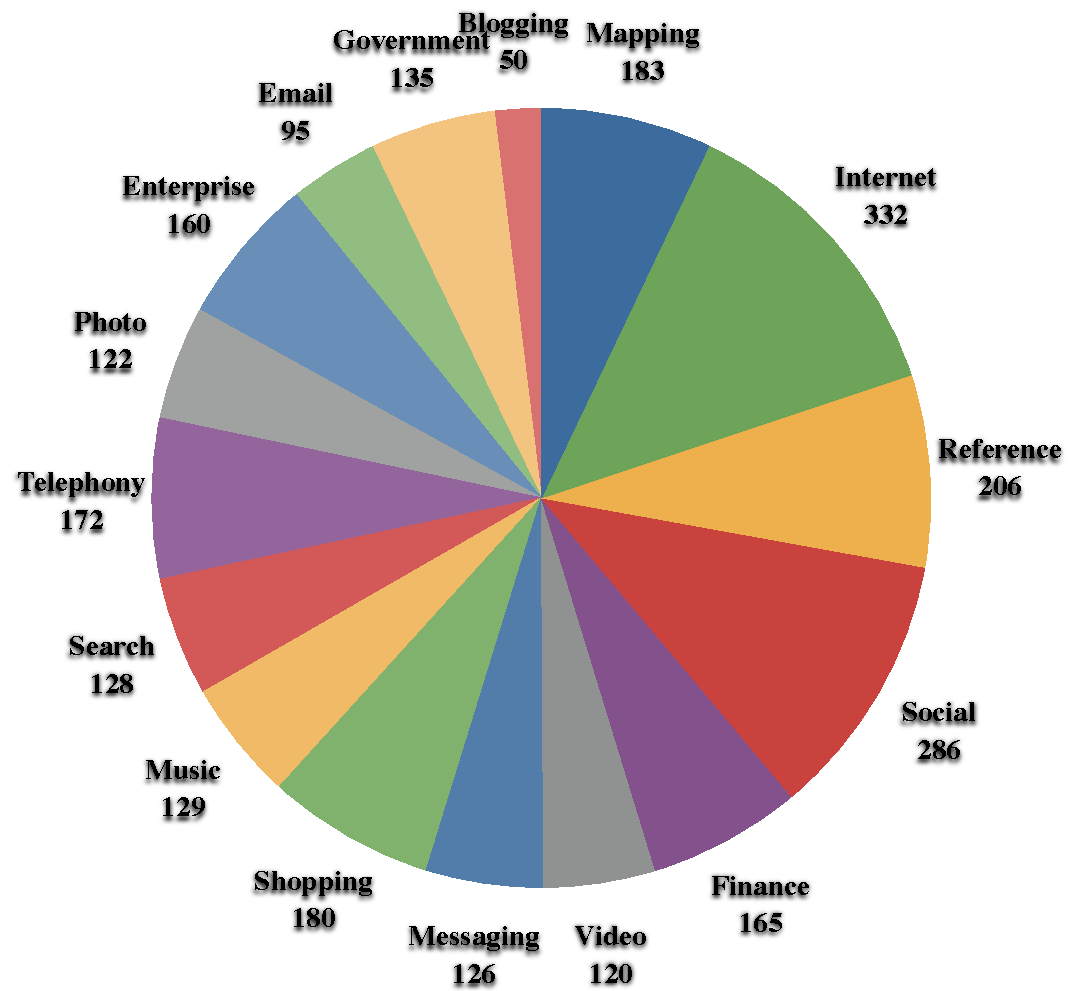
\includegraphics[width=.45\textwidth]{part1/pics/apis2011}\label{fig:api:2011}}
\end{center}
\caption{Data from~\cite{Domingue:2009} and actualized from ProgrammableWeb.com}
\label{fig:apis}
\end{figure}


{\bf Internet Of Services}\\
\label{subsec:ios}
Synergy is probably the best word to describe the \gls{ios} goal. Many services are now available on the Internet, such as hotel bookings, flight reservations or car rental. \gls{ios} aims to orchestrate the interactions of existing services to create new services more integrated, and dedicated to a task or a user. The goal is to create, for instance, a "Travels booking service" which aggregates the booking of a flight, hotel and car in a unique process.\\

Among all the "things" able to provide services, everyday life objects are also getting enriched with abilities to communicate through Internet-based technologies.\\

{\bf Internet Of Things}\\
\label{subsec:iot}
Stemming from the evolution of electronic devices, the \gls{iot} relates to an approach in which objects of everyday life have reached a sufficient level of maturity to interact one with each other. This interaction gives them the ability to act differently according to the situation 'sensed' with a stronger added value. Still in its infancy, the \gls{iot} is looking for software tools to develop and describe these interactions, as much as the services rendered.\\
Software components are quite suitable for virtualizing everyday life objects, and service-oriented computing is suitable for describing and implementing interactions. Software solutions developed in the future would probably merge both of these approaches. As long as it can be considered that a component offers services to other components, the collaboration of services and components produces promising results.\\

Information, devices and services are now able to communicate through the Internet, and render more and more integrated services to users. This strong integration requires all these services to be able to self-locate their dependencies, with no need for the user to set up technical properties (i.e.: server IP address, tcp port, etc...).\\

{\bf The Cloud}\\
\label{subsec:cloud}
Surfing on the service wave, hardware providers, software providers and others are offering more and more "things" as a service. Among others, \gls{saas} and \gls{paas} are the two main paradigms showing that everything can now be provided as a service.\\
The Cloud could be defined as the Internet of tomorrow. As everything is being served as a service, there is no more need to precisely locate services. Do you need a printer? Ask the cloud for the closest printer from you, and just use it. Might you need a lawyer? Ask the cloud for the best of them, and have a video-conference with him.\\
This approach makes it possible to obtain the hardware configuration you need, just-in-time, to run your software as a service. You will never know where your software is really run, but it will run in the cloud.\\

These principles are built on top of software architectures which basic elements are services or resources. Therefore, these approaches for building software are called Services-Oriented and Resource-Oriented architectures.

\subsubsection{Architectural principles}

In \cite{Papazoglou:2003}, M. Papazoglou defines Service-Oriented Architecture as "{\it a way of reorganizing software applications and infrastructure into a set of interacting services}". Services are able to describe themselves and realize computations for applications or other services, from a simple method execution to a complex business process. Services are offered by service providers which are responsible for the supply and support of their services. Clients of these services can be either applications or individuals, internally to the organization or from outside.\\
Possibly distributed over Internet, services must be {\it Technology Neutral} to be provided and used whatever the context, {\it Loosely coupled} to not rely on any specific context of use, and support {\it Location Transparency} by registering their location and description in directories such as UDDI, to allow clients to call the service regardless of its location.\\
%is a paradigm, an idea driving the way to develop software. Software services are rendering services to other services or individuals. If an application, or a software, uses services to achieve its goals, it is a service-based software.\\

%This section starts with some explanations about what is meant in this thesis by Service Oriented Architecture, and presents the S-Cube Network of Excellence, which funded this thesis. By the way, the last part of this section introduces to the new Internet of * paradigms.\\

{\bf SOA vs. WSOA}\\
In the Software Services community, service-oriented architecture is often used instead of web services-oriented architecture. However, there is a clear separation to respect between service-oriented architectures and web service.\\
Then, if a service is accessible through the Internet, this service is called web-service, and is a particular case of a service. Then service-oriented software can use this service as it would any other. \\
In conclusion, a service-based application does not necessarily use web-services and may even use no web service at all; there are other means of creating software based on services.\\

{\bf Web-Services}\\
A Web Service renders a service, using the Internet as a support. Web services are composed of methods that can be called by clients. Customers do not have to care about how the service is given and can just use it.\\
\begin{wrapfigure}{r}{.5\textwidth}
%	\vspace{-0.5cm}
  \centering
  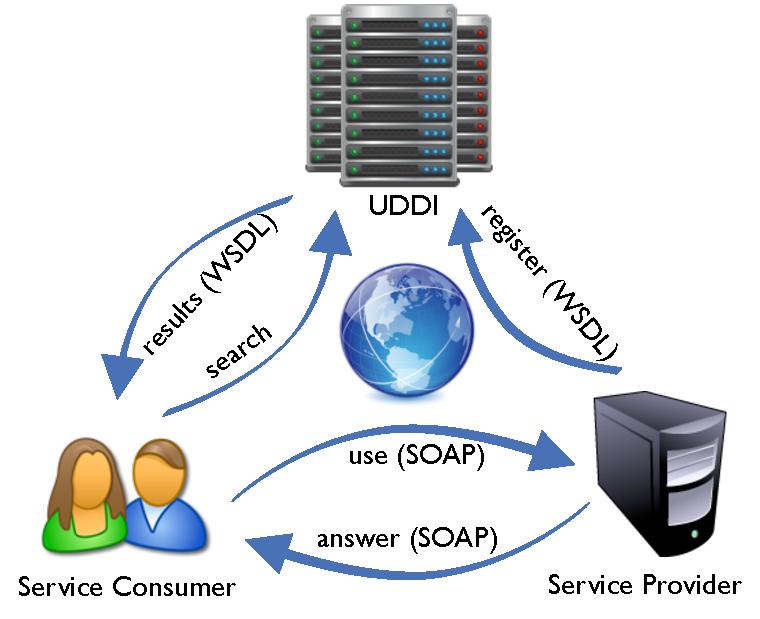
\includegraphics[width=.5\textwidth]{part1/pics/WSArchi.pdf}
  \caption{WebService Architecture}
  \label{fig:web-servce-archi}
%	\vspace{0.2cm}  
\end{wrapfigure}

The use of Web Services is based on a "search and use" mechanism. Service providers are responsible for the registration of their services into a \gls{uddi} directory. When a client wants to use a service, he first searches in a service directory. Each registered service comes with a description, which helps clients in their service selection process. The real call to the service is made directly from the client to the server. Figure~\ref{fig:web-servce-archi} illustrates this mechanism.\\

Registrations and descriptions of services in the \gls{uddi} are based on a description language for web services called \gls{wsdl}. The description of a service informs users about the list of operations offered, parameters, and types of objects manipulated. Dynamic discovery and use of services are enabled this way.\\
Communications between clients, servers and \gls{uddi} instances use a unique carriage protocol called SOAP. SOAP has been based on XML descriptions in order to make use of HTTP, SMTP, and other application protocols as carriers.\\

Although this approach provides mechanisms for dynamic search and use with precise descriptions, the amount of data exchanged and the complexity of the SOAP message structure can become an issue. Resource-limited platforms may not be able to embed a SOAP parser, or have a power supply designed to send a large amount of communication data. To cope with this problem, Resource-Oriented Architectures have been proposed.\\


{\bf Resources-Oriented Architectures}\\
%\label{sec:rest}

In his doctoral dissertation in 2000 \cite{Fielding:2000}, Roy Fielding introduced the term and idea of Representational State Transfer (REST).\\
REST has been designed to lighten transfers of information through web-based communications. Instead of heavy serializations of concrete program objects, REST architectures are share representations of these objects using XML for instance. These representations handle all coherent and meaningful information for the request (resp. answer) to be processed by the server (or client). REST defines only four standard CRUD \cite{Yoder:1998} operations to manage resources.\\
{\bf GET} is to retrieve the resource pointed by the called url. {\bf POST} asks the server to add the information contained in the request (hence a resource representation) to the resources pointed at the requested url. The {\bf PUT} operation is used to create or entirely replace a resource, based on the representation contained in the request. Finally, {\bf DELETE} requests the server to delete the specified resource.\\
URLs of REST servers handle information about the resource concerned by a request. For instance, a GET request on a URL such as {\it http://myMedia.org/} would be answered with an XML representation of the entire media library; a POST containing information about a new book, called on the {\it http://myMedia.org/books} would result in the addition of this book in the book library. As a final example, a DELETE request on {\it http://myMedia.org/books/2517} should remove the book whose unique identifier is 2517 from the book collection.\\
For its transportation, REST was initially described in the context of HTTP but is not limited to that protocol. Supported by an application-level transfer protocol, REST is thus development-technology agnostic.\\


Thanks to the appearance of these two paradigms, ideas emerged about connecting software systems and everyday life objects. The presence of registries or auto-discovery mechanisms also led to an abstraction of the details of the physical location. These interconnections finally brought new paradigms known as the Internet of *. 


\subsubsection{OSGi}
\label{subsec:osgi}

OSGi~\cite{OSGI:r4} is an association created in 1999 aimed to provide facilities for software integration and development.
To achieve this task, the association released a set of specifications defining what any runtime implementation should do to reach a given service level. These specify which minimum set of services a runtime must offer to be compliant with the level.\\
In OSGi, services are given and contained in deployments units called {\it bundles}. Each bundle contains a {\it Manifest} file giving information about the runtime dependencies, the classes offered and some other information about what the bundle needs to run. Bundles can be installed, updated or removed at any time and their services can be started and stopped, with no need to restart the runtime platform.\\
Services are defined by Java interfaces (for Java runtime implementations), and are stored in the runtime context. Thus, any client on the platform who needs a service can search in the context registry for the service they need. Service method calls are locally handled inside a JVM, which makes this service-oriented runtime much faster than web service-based applications.\\

In OSGi, relations between bundles are never made explicit. Worse still, relations between bundles can be due to service dependencies that are just hard-coded and can only be changed by rebuilding and redeploying the bundle. In a static application, with few updates in time, this is not a real problem. Moreover, there are very few reflection primitives and thus, interactions between bundles can hardly be traced or even made explicit. OSGi do not address issues of interoperability, variability management nor safety and security. The registry mechanism is a good point concerning openness, and adaptations and evolutions of applications are simplified by the native lifecycle management of OSGi. In a word, OSGi lacks of a clear means of visualization of the architecture while running, but makes a very good base.\\

The table below is completed for each approach or tool, and presents strengths and weaknesses in a synthetic way. Individual tables are merged altogether in section~\ref{ch:summary} as a synthesis. \\
 \\
\begin{tabular}{ >{\centering}m{.13\textwidth}| >{\centering}m{.09\textwidth} >{\centering}m{.12\textwidth}| >{\centering}m{.10\textwidth} >{\centering}m{.20\textwidth}| >{\centering\arraybackslash}m{.15\textwidth}}
{\tiny Interoperability} & {\tiny Openness} & {\tiny Adaptation} & {\tiny Evolution} & {\tiny Variability Management} & {\tiny Safety \& Security}\\
 \hline
  & + & + & + &  & \\ 
  \hline
\end{tabular}\\


\subsubsection{Enterprise Service Bus}

\gls{esb} refers to a business middleware family for service-oriented applications. This middleware acts as the only mediator of services in the enterprise, by providing a runtime environment for deploying business services. Legacy software can be integrated as services into the business service orchestration. These are declared as any other service, within the scope of the ESB runtime. The specifications have been successfully implemented in several frameworks such as OpenESB by SunMicrosystems, ServiceMix by Apache Foundation, or Petals by OW2.\\
\gls{jbi} or JSR 208 is an industrial Java standard developed to ease the integration of software systems over Service-Oriented Architectures. It uses an \gls{esb} as a basis to define a component model. It has been designed to reuse Java technologies such as WebServices, BPEL or JMS, and thus avoid new specific developments.  
In \gls{jbi}, components have an independent life-cycle and communicate through their services over normalized message middleware. In fact, this middleware acts as an abstraction layer for communications and eases the integration. \gls{jbi} components are split into two categories:\\
{\bf Service Engine Components} are directly hosted by the \gls{jbi} runtime environment, and are in charge of message processing, routing or orchestration of services. They cannot communicate outside of this scope.\\
{\bf Binding Components} expose or consume standard \gls{jbi} services, and perform the bindings with external non-standard software.\\
The packaging as components is described in the framework like this: service descriptions are encapsulated into Service Units, which are then encapsulated into deployable business components called Service Assemblies.\\
 
The message middleware makes \gls{jbi} a serious candidate in terms of interoperability of components. Openness is offered by the Binding Components, and evolutions are natively supported thanks to its service-oriented nature.
Besides its good properties, there is no clear separation between types and instances of services/components. Moreover, no introspection of services is offered and interconnections between components are not explicitly expressed, and sometimes even hard-coded inside the components.
This lack of clarity in the component interdependencies makes it impossible to dynamically replace components and/or reason about the system's state. This approach do not target the resolution of variability management or safety and security issues.\\
 \\
\begin{tabular}{ >{\centering}m{.13\textwidth}| >{\centering}m{.09\textwidth} >{\centering}m{.12\textwidth}| >{\centering}m{.10\textwidth} >{\centering}m{.20\textwidth}| >{\centering\arraybackslash}m{.15\textwidth}}
{\tiny Interoperability} & {\tiny Openness} & {\tiny Adaptation} & {\tiny Evolution} & {\tiny Variability Management} & {\tiny Safety \& Security}\\
 \hline
 + & + &  & + &  & \\ 
  \hline
\end{tabular}\\


%\newpage
\subsection{Component models}
\label{sec:componentModelStateOfArt}
\vspace{0.3cm}


\subsubsection{Description}

Douglas McIlroy first introduced the notion of software component in 1968 at the NATO conference. This new paradigm defends a mass reuse of existing components and the creation of software as assemblies of components.\\
As described in \cite{Medvidovic:2000}, component models are made of three essential elements. A {\it Component} represents a computational unit and can realize an entire application or a single method. Components have a type and expose interfaces to collaborate with other components. This collaboration is enabled by component {\it Connectors}, in charge of the communication between the application's components. These connectors are typed and can have different behaviors, roles in the application, and can make use of various techniques to support components' interactions. Finally, a {\it Configuration} describes a particular assembly of components and connectors, and specifies the component-base software system.\\
The next section provides a brief list of component models.\\

\subsubsection{Darwin}

In~\cite{Georgiadis:2002} Ioannis Georgiadis and al. present a component model to describe self-organizing software architectures of distributed systems. In this model, components are defined by component types and can have multiple runtime instances. Instances can be statically specified at design time, or created on demand at runtime.
Usually, components provide and require services. The provision or requirement is made through typed ports. These types are specified by the interface of the service they offer.
Components are connected by their ports and the semantics of bindings is a classical service call. Obviously, port types have to be the same. Components can be assembled into composite components. Their specifications describe the instances used and how they are connected.\\
At runtime, component instances embed a view of the global configuration and a manager handling the architecture constraints, in charge of maintaining the configuration view synchronized with the system state.\\

The clear separation of types and instances is a plus. Runtime creation of instances can help in adapting the runtime to the environment. The configuration view synchronized with the runtime is a very interesting property. The use of Java class loading to change utility functions used by the policy manager is a good way to runtime evolution.\\
If the typing of ports is helpful to guarantee the consistency of an application model, the typing at the implementation level can act against the interoperability property, but enforce the safety of the system. Bindings have a clear semantic, but cannot use other communication links than the one they have been designed to use (Java RMI in this case). It is a limitation. The adaptation policies (in case of binding loss or component arrival for instance) are hard coded and distributed in each instance. Thus they cannot be easily changed at runtime.\\
\\
\begin{tabular}{ >{\centering}m{.13\textwidth}| >{\centering}m{.09\textwidth} >{\centering}m{.12\textwidth}| >{\centering}m{.10\textwidth} >{\centering}m{.20\textwidth}| >{\centering\arraybackslash}m{.15\textwidth}}
{\tiny Interoperability} & {\tiny Openness} & {\tiny Adaptation} & {\tiny Evolution} & {\tiny Variability Management} & {\tiny Safety \& Security}\\
 \hline
  &  & + & + &  & + \\ 
  \hline
\end{tabular}\\


\subsubsection{Koala}

The Koala component model has been designed to handle the increasing diversity and complexity of embedded software and decrease development costs. Rob van Ommering and al. explain in ~\cite{RobVanOmmering:2000} that a way to achieve this is to model the software architecture and reuse existing software components rather than re-implementing the wheel. In their approach, a clear separation is made between component development and system configuration. It means that component developers cannot make any assumption about the context of use of each component and designers cannot change component behavior.\\
Components can require services provided by other component's ports.
A configuration describes an assembly of components. It handles the model of the application. To help in describing system assembly, Koala offers compound components in which  instances to be deployed and their interactions (bindings) are described. In this case, an action on a port of the compound component may have to be forwarded to internal components (e.g.: for initialization). To eliminate the ordering problem, Koala introduced {\it Modules} to handle one-to-many, many-to-one or many-to-many bindings. They are in charge of propagation and have a pre-defined treatment.\\

The clear separation between component development and assembly creation (for a particular application) is the key to success. Composition mechanisms are also welcome to cope with diversity management and promote the reuse of existing components to create value-added compound components. Here again, connection ports are typed and should conform to a specific interface. This is an advantage for securing the software but may cause problems in future evolutions, in terms of interoperability. Koala introduced modules to handle specific communications between components and act like a proxy. They could have gone a bit further by systematically using modules to specify each connection. This information could help in solving issues, or in specifying the system more precisely.\\
\\
\begin{tabular}{ >{\centering}m{.13\textwidth}| >{\centering}m{.09\textwidth} >{\centering}m{.12\textwidth}| >{\centering}m{.10\textwidth} >{\centering}m{.20\textwidth}| >{\centering\arraybackslash}m{.15\textwidth}}
{\tiny Interoperability} & {\tiny Openness} & {\tiny Adaptation} & {\tiny Evolution} & {\tiny Variability Management} & {\tiny Safety \& Security}\\
 \hline
  &  &  & + & + & + \\ 
  \hline
\end{tabular}\\

\subsubsection{Fractal}

%Paragraph extracted from SEAA'10
Fractal~\cite{Bruneton:2006} is a modular and extensible component model to design, implement, deploy and reconfigure various systems and applications. Famous implementations of Fractal are Julia and AOKell (Java), Cecilia (C), FractNet (.NET) and FracTalk (SmallTalk).\\
The Fractal component model supports the definition of primitive and composite components. Each Fractal component consists of two parts: a controller, which exposes the component's interfaces, and content, which can be either a user class or other components in composite components. The model makes the bindings between the interfaces provided or required by these components explicit, as well as the hierarchic composition (including sharing).\\
Primitive components contain the actual code and composite components are only used as a mechanism to deal with a group of components as a whole, while potentially hiding some of the features of the subcomponents. Primitives are actually standard Java classes (in the Java distributions of Fractal) conforming to some coding conventions. Fractal does not impose any limit on the levels of composition, hence its name.\\
All interactions between components pass through their controller. The model thus provides two mechanisms to define the architecture of an application: bindings between interfaces of components, and encapsulation of a group of components into a composite. By default, Fractal proposes 6 controllers that may be present in components: Attribute, Name, Binding, Content, Lifecycle and Super Controller.\\
DigiHome\cite{Romero:2010} is a communication middleware built with Fractal. Its main objective is to offer a support for REST communications, and complex event processing, in a context of home automation.

Reflective execution platforms like Fractal or OpenCOM \cite{Blair:2004} do not provide a clear distinction between the reflection model and the reality. 
Modifying the reflection model implies a modification in the runtime. If this offers a means for adapting the runtime, there is no means to anticipate the effect of a reconfiguration, before actually executing it. Nor is there means to execute what-if scenarios to evaluate different possible configurations, etc. This point is a drawback from a safety viewpoint.
This lack of an explicit and independent reflection model imposes that most of the verifications must be carried out while reconfiguring. Pre-condition on reconfiguration actions, as proposed by L\'eger \cite{Leger:2007}, are checked and roll-backs are performed if something goes wrong.
In addition, component models such as Fractal are slightly opaque with respect to the outside world, making openness and reuse by third party applications complicated if not anticipated in advance. Lastly, the dynamicity of an application running over Fractal is compromised, because the deployment of new component' types can not be carried out without restarting.\\
 \\
\begin{tabular}{ >{\centering}m{.13\textwidth}| >{\centering}m{.09\textwidth} >{\centering}m{.12\textwidth}| >{\centering}m{.10\textwidth} >{\centering}m{.20\textwidth}| >{\centering\arraybackslash}m{.15\textwidth}}
{\tiny Interoperability} & {\tiny Openness} & {\tiny Adaptation} & {\tiny Evolution} & {\tiny Variability Management} & {\tiny Safety \& Security}\\
 \hline
  &  & + &  &  &  \\ 
  \hline
\end{tabular}\\


\newpage
\subsection{Component Models for SOA}

\subsubsection{Description}

By nature, Service-Oriented software is dynamic and its architecture is not always easy to figure out. Indeed, the services used and the connections between software elements are never known prior to the execution because of the late binding principle. The late binding principle relates to the fact that a service to be used is searched and selected just before its call. Component models for \gls{soa} have been invented to try to make the description of this kind of application more explicit. They merge well-known software component techniques with new services ideas, and tend to conciliate the best of each approach.\\

Components, as defined by component models, provide services to other components through their ports. Components' ports are defined by an API. Services, from service-oriented architectures are intended to be used in orchestrations to create value-added applications.\\
Since both of these concepts offer services, new component models have been designed to merge both paradigms. This section presents some famous implementations of these component models.\\

\subsubsection{SCA}

\gls{sca}\footnote{http://www.osoa.org/} provides a component model for both the composition of services and for the creation of service components.
\gls{sca} is a model that aims to encompass different programming languages, frameworks and environments commonly used to build components and services, such as Web Services, Messaging systems and \gls{rpc} for communication purposes. Its goal is to setup a single and common way to access and assemble service-based applications.\\
\gls{sca} can be presented through four major parts of the specification.\\

{\bf Specifications}\\
\par {\bf Assembly} defines how components are packaged as services and how they can be combined into composites that perform a particular task.
Composite components can be used as classical service components, which simplifies their reuse. Assembly in \gls{sca} also defines how components and composites are connected. Functional service properties, such as data encryption, or authentication, are described outside the service business code, which saves developers' valuable time. Indeed, it enables the modification of the connections or the properties, without changing the business code.
\par {\bf Client and Implementation Model} defines how services are packaged and accessed in various languages. API implementations in Java, BPEL, C++, Javascript or the Spring Framework, offer means to package a service or access any \gls{sca} service. For development concerns, it means that there is only one interface and packaging method to learn to provide and use any \gls{sca} service. This interface makes it possible to access to the component using Web services, JMS, JCA and EJBs natively. Here again, service properties are described outside the code, to make changes much easier.
\par {\bf Policy Framework} is aimed at offering means for the definition of security, authentication, quality of service, and other important policies of a service. In fact, the \gls{sca} Policy Framework makes use of the WS-Policy and WS-Policy Framework open standards, as a support to describe policies. This way, descriptions of policies such as "any data sent to this service must be encrypted" or "the user of this service must be authenticated" are made available. Here again, policies can be defined outside the business code of the service.
\par {\bf Bindings} specify the mechanisms that can be used to access or connect a component. Bindings can be implemented using Web services, JMS, JCA, EJBs or any other communication way. Keeping the consistency of the approach, bindings are defined outside the component business code.\\

SCA is a standard, a set of definitions describing how such a system should behave. Thus, it imposes certain types of implementation, in order to guarantee the presence of mechanisms for openness, evolution or remote control.\\
\\
\begin{tabular}{ >{\centering}m{.13\textwidth}| >{\centering}m{.09\textwidth} >{\centering}m{.12\textwidth}| >{\centering}m{.10\textwidth} >{\centering}m{.20\textwidth}| >{\centering\arraybackslash}m{.15\textwidth}}
{\tiny Interoperability} & {\tiny Openness} & {\tiny Adaptation} & {\tiny Evolution} & {\tiny Variability Management} & {\tiny Safety \& Security}\\
 \hline
  & + &  & + &  & + \\ 
  \hline
\end{tabular}\\


\subsubsection{FraSCAti}

FraSCAti~\cite{Melisson:2010} is an implementation of the SCA specifications. It is certainly the closest approach to what is required. Components can be composed into composite components. Communications between components are made using services and several communication media can be used. These elements make FraSCAti a serious candidate to address openness and remote control concerns.\\
In the past months, efforts have been spent on integrating FraSCAti and OSGi, which have improved its faculties of evolution. In terms of interoperability, FraSCAti offers mechanisms for the connection of services, but does not directly address the integration of smart devices. Thus, interoperability of components in our context is still compromised by the use of APIs, for the definitions of services rendered and required, by ports. If two components have not been designed to be connected, an ad-hoc connector has to be created.\\
The FraSCAti script tool enables reconfiguration and adaptation of component assemblies. But adaptations are limited to the manipulation of binding and component instances, whose types are available on the platform. New instances can be created, new bindings can be set, but no new types can be installed using FraSCAti Script.\\
The variability of FraSCAti itself is managed using a Software Product Line(SPL). Each runtime instance of FraSCAti is a product of the SPL. Thus, features of FraSCAti can be deployed on demand. However, this variability management concerns only the internal features of FraSCAti, and an external tool is still required to handle the variability of applications made with FraSCAti.\\
\\
\begin{tabular}{ >{\centering}m{.13\textwidth}| >{\centering}m{.09\textwidth} >{\centering}m{.12\textwidth}| >{\centering}m{.10\textwidth} >{\centering}m{.20\textwidth}| >{\centering\arraybackslash}m{.15\textwidth}}
{\tiny Interoperability} & {\tiny Openness} & {\tiny Adaptation} & {\tiny Evolution} & {\tiny Variability Management} & {\tiny Safety \& Security}\\
 \hline
 + & + &  & + &  & + \\ 
  \hline
\end{tabular}\\

\subsubsection{iPOJO}
iPOJO~\cite{Escoffier:2007} is the Apache service-oriented component runtime built on top of OSGi \gls{soa} platforms. iPOJO is the natural evolution of the Service Binder mechanism introduced by Cervantes et al. in~\cite{Cervantes:2004}. The iPOJO framework merges the advantages of component- and service-oriented paradigms. Specifically, application functionalities are implemented following the component paradigm. Each component is fully encapsulated, self-sufficient, and provides server and client interfaces as services. An iPOJO component is actually managed by a reusable container, which provides common middleware functionalities. Each component container can be configured with a different set of middleware services.\\
The iPOJO component model focus on providing management facilities for pervasive applications based on component model, and a service-oriented runtime. This general purpose component model for service oriented architectures provides a solid base for domain specific extensions and developments.
 \\
\begin{tabular}{ >{\centering}m{.13\textwidth}| >{\centering}m{.09\textwidth} >{\centering}m{.12\textwidth}| >{\centering}m{.10\textwidth} >{\centering}m{.20\textwidth}| >{\centering\arraybackslash}m{.15\textwidth}}
{\tiny Interoperability} & {\tiny Openness} & {\tiny Adaptation} & {\tiny Evolution} & {\tiny Variability Management} & {\tiny Safety \& Security}\\
 \hline
  & + & + & + &  & \\ 
  \hline
\end{tabular}\\


\newpage
\section{Domain-specific approaches}
\label{sec:domainSpecificApproaches}

General purpose approaches make it possible to design and implement software solutions for many problems. But this flexibility comes with a complexity due to the knowledge required to be able to develop or simply use these approaches.\\

Domain-specific approaches tend to reduce this complexity to a minimum, by providing tools on top of general purpose approaches adapted to a specific domain of use. In this section, several tools built upon this principle are reviewed to list their advantages and disadvantages.

\subsection{Description}
\label{sec:mdeEtDSL}


\gls{mde} is an approach that promotes the use of an abstract representation of a piece of software, before its actual realization. From this abstract view, tools and methods make it possible to automate the final software generation, tests and validations across pre-defined requirements. Models are human understandable representations of reality. They can handle information about structure, data exchange, communication links, or some building constraints of a piece of software.\\
\gls{dsl} are another means of abstraction and description of software systems. Dedicated to a specific domain, they can be graphical, textual or both. They are designed to restrict the concepts manipulated to the ones from the application domain. This approach makes it easier for domain specialists to express a software system architecture and behavior, by using their own terminology.\\

The goal of these tools is to provide a sufficient level of abstraction to make software development easier, more flexible, with an enhanced level of reliability, and shorter time-to-market.\\
The rest of this section presents several approaches built around the concepts of \gls{mde} and/or \gls{dsl}, that simplify the creation of applications in the domain of home automation and/or pervasive computing.\\


\subsection{Projects}

\subsubsection{uMiddle}
Nakazawa et al propose a framework that bridges remote smart spaces called D-uMiddle in~\cite{Nakazawa:2007}. This makes it possible for a device to interact with another, over the Internet. This is made available by four distinct features of D-uMiddle. Firstly, a local mapper mechanism abstracts sensor nodes into common representations. Secondly, a mechanism translates data transmission protocols from a node-specific one to a D-uMiddle common one. Thirdly, a remote mapper mechanism creates proxies of sensor nodes from remote smart spaces in the local space. Fourthly, a transport module enables devices to receive data over IPv4 NATs network. The consumer devices, as a result, can use sensor nodes in remote smart spaces without depending on their own protocols and semantics, and without being burdened by the complicated IPv4 NATs.\\

D-uMiddle brings a solution for connecting remote smart spaces, with no need for a developer to care about transportation. Remote control of equipment is thus made possible for free. Nevertheless, it does not supply tools to handle variability, adaptation or evolution of a deployed system, and nothing is specified about the securization of the connection.\\
 \\
\begin{tabular}{ >{\centering}m{.13\textwidth}| >{\centering}m{.09\textwidth} >{\centering}m{.12\textwidth}| >{\centering}m{.10\textwidth} >{\centering}m{.20\textwidth}| >{\centering\arraybackslash}m{.15\textwidth}}
{\tiny Interoperability} & {\tiny Openness} & {\tiny Adaptation} & {\tiny Evolution} & {\tiny Variability Management} & {\tiny Safety \& Security}\\
 \hline
  &  &  &  &  & \\ 
  \hline
\end{tabular}\\

\subsubsection{SOPRANO}
SOPRANO (Service-Oriented Programmable Smart Environments for Older Europeans) was an Integrated European Project, which successfully ended in April 2010. Its main achievement was the release of openAAL~\cite{Wolf:2010}, a framework built on top of an OSGi execution platform. OpenAAL helps in getting information from devices, and acting on them from a higher level of abstraction. Its framework integrated a context manager, able to give a virtual view of all devices, a process manager in charge of making decisions for any change in the context, and a composer, dealing with the actual services for interaction with the real environment.\\

OpenAAL proposes a solution to efficiently built applications ready to evolve with needs and able to adapt to changes in context. However, no attention is paid to the variability management, remote control or interoperability of devices. Nothing is said about safety of security.\\
 \\
\begin{tabular}{ >{\centering}m{.13\textwidth}| >{\centering}m{.09\textwidth} >{\centering}m{.12\textwidth}| >{\centering}m{.10\textwidth} >{\centering}m{.20\textwidth}| >{\centering\arraybackslash}m{.15\textwidth}}
{\tiny Interoperability} & {\tiny Openness} & {\tiny Adaptation} & {\tiny Evolution} & {\tiny Variability Management} & {\tiny Safety \& Security}\\
 \hline
  &  & + & + &  & \\ 
  \hline
\end{tabular}\\


\subsubsection{Ga\"ia Framework}
Ga\"ia~\cite{Roman:2002} is presented as a meta-operating system for ubiquitous computing, built on top of a classical operating system. Its goal is to detach itself from the heterogeneity and complexity associated to ubiquitous environments. Ga\"ia is composed of a Kernel, responsible for the runtime management of applications and a Framework to build these applications. An application runs in an Active Space, a physically-limited space where services and devices are available for ubiquitous computing.\\
Each Ga\"ia instance is specifically configured for the active space it manages. To allow for describing Ga\"ia applications for several active spaces, Olympus\cite{Ranganathan:2005} proposes a high-level DSL working with virtual entities. From an Olympus application model, the underlying Ga\"ia OS takes responsibility for mapping each virtual entity to a service, or device, available in the active space.\\
It has been implemented in CORBA and can be ported to other communication middleware architectures such as SOAP or RMI.\\

The interoperability of services and devices is ensured by the common set of basic services. Adaptations and evolutions are made possible by the Component Management Core of Ga\"ia which can dynamically load, transfer, create or destroy components or applications. Remote control is made available by the underlying CORBA platform, in the implementation described. Variability management of components or applications, safety and security, and openness of the solution are not targeted by this work.\\
\\
\begin{tabular}{ >{\centering}m{.13\textwidth}| >{\centering}m{.09\textwidth} >{\centering}m{.12\textwidth}| >{\centering}m{.10\textwidth} >{\centering}m{.20\textwidth}| >{\centering\arraybackslash}m{.15\textwidth}}
{\tiny Interoperability} & {\tiny Openness} & {\tiny Adaptation} & {\tiny Evolution} & {\tiny Variability Management} & {\tiny Safety \& Security}\\
 \hline
 + &  & + & + &  &  \\ 
  \hline
\end{tabular}\\


\subsubsection{DiaSuite}
DiaSuite\footnote{http://phoenix.inria.fr/projects/diasuite} is a software tool suite designed to ease the creation of pervasive and/or distributed applications. DiaSuite~\cite{CASSOU:2010} is composed of several elements. DiaSpec is the \gls{adl} of the suite, used to describe the applications at a convenient level of abstraction. From this description, DiaGen automates the code generation of the application, and DiaSim provides the support for the test, simulation and validation of the generated application. As an example, Bertrand et al. present in \cite{BERTRAN:2010} how they used the SIP protocol as a generic communication bus for a pervasive application developed with DiaSuite tools.\\
This tool suite has been augmented with Pantagruel\footnote{https://pantagruel.bordeaux.inria.fr/}, a visual \gls{dsl} created to support the development of pervasive applications. A first step when using Pantagruel aims at defining the entities involved in the future application domain. In a second step, entities of the application are orchestrated in order to define the logic of the application. A last step generates an application code, compatible with the DiaSuite tools. Details about this tool are available in \cite{DREY:2009}.\\


These tools meet the demands of a tool chain to develop pervasive applications from a high-level description. Code generation and the simulation environment are very good tools to improve the efficiency of the development process and the reliability of the code, as much as facing the variability of solutions. Designed to ease the development of pervasive applications, these tools do not address issues about variability management, application evolutions or adaptations.\\
\\
\begin{tabular}{ >{\centering}m{.13\textwidth}| >{\centering}m{.09\textwidth} >{\centering}m{.12\textwidth}| >{\centering}m{.10\textwidth} >{\centering}m{.20\textwidth}| >{\centering\arraybackslash}m{.15\textwidth}}
{\tiny Interoperability} & {\tiny Openness} & {\tiny Adaptation} & {\tiny Evolution} & {\tiny Variability Management} & {\tiny Safety \& Security}\\
 \hline
 + & + &  &  & + & + \\ 
  \hline
\end{tabular}\\


\subsubsection{Habitation}
Habitation is a methodology, a set of tools to address the specific requirements of home automation application development and design. In \cite{Jimenez:2009}, Jimenez et al. describe how the combination of a \gls{dsl}, and an \gls{mde} approach eases the creation of solutions in this domain. Habitation proposes three main tools. A catalog of functional units centralizes elements that can be reused in various applications. Home automation devices are composed of several functional units. The second tool is a workspace in which elements of the catalog can be placed to define a specific application. Called the application view, this tool aims to provide tools for the assembly work and make it accessible for non-domain experts. The last tool is a kind of engine, which translates from the model and \gls{dsl} description, to a technology-specific configuration file.\\


The approach proposed by Habitation is very promising and sounds helpful in providing non-expert users with tools having a sufficient level of abstraction to be user friendly. However, Habitation only addresses pre-deployment design issues and does not deal with issues such as evolutions, adaptations and safety and security issues. Such as DiaSuite, Habitation remains an good approach to face the variability issue, while improving the efficiency of the development process.\\
\\
\begin{tabular}{ >{\centering}m{.13\textwidth}| >{\centering}m{.09\textwidth} >{\centering}m{.12\textwidth}| >{\centering}m{.10\textwidth} >{\centering}m{.20\textwidth}| >{\centering\arraybackslash}m{.15\textwidth}}
{\tiny Interoperability} & {\tiny Openness} & {\tiny Adaptation} & {\tiny Evolution} & {\tiny Variability Management} & {\tiny Safety \& Security}\\
 \hline
 + &  &  &  & + & \\ 
  \hline
\end{tabular}\\


\subsubsection{Wired Application Description Language}
Wired Application Description Language(WADL) is a language designed to ease the description of dynamic applications, and provide an explicit view of the relations between elements. In \cite{Cervantes:2008} authors present how WADL has been used in the creation of a dynamic sensor-based application.\\
WADL has been implemented on OSGi(see section~\ref{subsec:osgi}) and relies on the WireAdmin service offered by the execution platform. In this implementation, wires between producers of information and consumers are dynamically created or deleted, according to the elements available in the system. Wires are specified by two filters. Each filter is used to make a selection among all available services, and capture producers' (or consumers') services required for the wire.\\

WADL provides a tool to explicit the architecture of dynamic applications, which is often difficult to extract because of the runtime evolutions. By nature, this approach copes with the adaptation requirement. The interoperability is realized by the use of a Producer/Consumer pattern. Evolution is supported by the filters that can be flexible enough to admit future evolutions. Issues on openness, variability management and safety and security are not treated in this approach.\\
\\
\begin{tabular}{ >{\centering}m{.13\textwidth}| >{\centering}m{.09\textwidth} >{\centering}m{.12\textwidth}| >{\centering}m{.10\textwidth} >{\centering}m{.20\textwidth}| >{\centering\arraybackslash}m{.15\textwidth}}
{\tiny Interoperability} & {\tiny Openness} & {\tiny Adaptation} & {\tiny Evolution} & {\tiny Variability Management} & {\tiny Safety \& Security}\\
 \hline
 + &  & + & + &  & \\ 
  \hline
\end{tabular}\\


\subsubsection{PervML}
Mu\~nos et al. present PervML in~\cite{Munoz:2006a,Munoz:2006b} in the context of the management of a pervasive meeting room. PervML is a Model Driven Approach designed to ease the development of pervasive systems. This language separates the analyst's view, describing the requirements of the system at a high level of abstraction, from the architect's view, where devices and implementation details are specified.\\
This abstract model of the system is then used in a tool chain which ends up with an executable OSGi(see section~\ref{subsec:osgi}) code. This tool chain, detailed in \cite{Munoz:2006}, firstly transforms the platform independent PervML model to an OSGi dependent model, and then generates the executable Java code.\\
PervML and the associated generation tool chain are available as a plugin for Eclipse \cite{Cetina:2007}.\\
In \cite{Serral:2010a}, authors explain how they introduced system evolution capabilities to adapt the generated systems to changes in user behavior. Their solution uses a context model, to detect specific situations, and a task model describing the jobs to be executed for each detected context.\\

PervML offers a suitable solution. Developed to be executed on an OSGi platform, it naturally offers adaptation, evolution, openness and interoperability mechanisms. As presented in \cite{Cetina:2009}, PervML also targets the variability management issue. So far, a drawback of this approach is that people have to be familiar with UML to model a pervasive application. Also, the use of a pre-defined set of service interfaces described in the framework may become a barrier for the flexibility of the solution. Safety and security issues are not addressed by this work.\\
\\
\begin{tabular}{ >{\centering}m{.13\textwidth}| >{\centering}m{.09\textwidth} >{\centering}m{.12\textwidth}| >{\centering}m{.10\textwidth} >{\centering}m{.20\textwidth}| >{\centering\arraybackslash}m{.15\textwidth}}
{\tiny Interoperability} & {\tiny Openness} & {\tiny Adaptation} & {\tiny Evolution} & {\tiny Variability Management} & {\tiny Safety \& Security}\\
 \hline
 + & + & + & + & + & \\ 
  \hline
\end{tabular}\\




\subsubsection{AutoHome}

In~\cite{Bourcier:2011}, Bourcier et al. present AutoHome as an autonomic management framework for pervasive home applications. AutoHome is described as a middleware that extends the iPOJO component model, to create a framework to host autonomic home applications. Using this approach, authors aim to separate the design and development of the application itself, from autonomic management components. They aim to enable the development of autonomic management functions, ease their integration with the applications, and finally, deploy the resulting autonomic application on execution environments shared with other applications. As a consequence, an application on top of AutoHome has the following architectural elements: middleware offering an autonomic service-oriented component and a context facility, a runtime that includes monitoring and reconfiguration abilities, a set of service-oriented applications which represent pervasive components to be autonomously managed, and a set of managers organized in a hierarchy.\\

AutoHome makes it possible to include, within the application itself, specialized components that monitor and react on component or platform events.
However, this solution does not seem to offer means for variability management, or interoperability between components, and does not consider safety or security aspects.\\
 \\
\begin{tabular}{ >{\centering}m{.13\textwidth}| >{\centering}m{.09\textwidth} >{\centering}m{.12\textwidth}| >{\centering}m{.10\textwidth} >{\centering}m{.20\textwidth}| >{\centering\arraybackslash}m{.15\textwidth}}
{\tiny Interoperability} & {\tiny Openness} & {\tiny Adaptation} & {\tiny Evolution} & {\tiny Variability Management} & {\tiny Safety \& Security}\\
 \hline
  & + & + & + &  & \\ 
  \hline
\end{tabular}\\


\subsubsection{WComp}

WComp\cite{Ferry:2011uq,Tigli:2009} is a component model designed to support ubiquitous computing. It tries to address issues introduced by the mobility of devices, their heterogeneity and the dynamicity of the execution environment in this domain. To cope with these problems, WComp federates three paradigms. Event-Based Web Services, firstly, that plays an important role in facing the heterogeneity of devices, as much as the dynamicity, the extensibility and scalability of a ubiquitous system. Secondly, a Lightweight component-model (called SLCA) is introduced and used to compose event-based Web services, and expose a new service. The third paradigm used concerns the adaptation and makes use of the Aspect of Assembly concept. These aspects define adaptations on assemblies using structural descriptions. Adaptation are thus not specific to particular service assemblies and can be composed.\\

WComp offers several mechanism for adaptations, evolutions and interoperability,  and does not seem to address openness, variability management and safety or security concerns. Finally, it looks like the type system of the components rely on the implementation language type system, which can limit the reuse and interoperability.\\
 \\
\begin{tabular}{ >{\centering}m{.13\textwidth}| >{\centering}m{.09\textwidth} >{\centering}m{.12\textwidth}| >{\centering}m{.10\textwidth} >{\centering}m{.20\textwidth}| >{\centering\arraybackslash}m{.15\textwidth}}
{\tiny Interoperability} & {\tiny Openness} & {\tiny Adaptation} & {\tiny Evolution} & {\tiny Variability Management} & {\tiny Safety \& Security}\\
 \hline
 + &  & + & + &  & \\ 
  \hline
\end{tabular}\\

\subsubsection{Niagara}

NiagaraAX is a software framework and a development environment that leverage the accessibility of a device toward an Internet access. 
The normalization proposed by NiagaraAX of the behavior and data gathered from several devices, enables the implementation of seamless, Internet-connected, web-based systems, whatever their manufacturer or communication protocol. This normalization has been enabled by the Niagara's unique, patented component model that transforms the data from diverse external systems into uniform software components.
These components share the foundation for building applications to manage and control the devices.\\

NiagaraAX eases the creation of applications integrating services and devices, by providing a framework for the development of drivers and applications. Built as a service-oriented architecture, this framework promotes the interoperability of devices and openness of solutions through Internet-based communications. NiagaraAX does not target issues about adaptations of the software or its evolution at runtime. Safety and security are not part of this work.\\
 \\
\begin{tabular}{ >{\centering}m{.13\textwidth}| >{\centering}m{.09\textwidth} >{\centering}m{.12\textwidth}| >{\centering}m{.10\textwidth} >{\centering}m{.20\textwidth}| >{\centering\arraybackslash}m{.15\textwidth}}
{\tiny Interoperability} & {\tiny Openness} & {\tiny Adaptation} & {\tiny Evolution} & {\tiny Variability Management} & {\tiny Safety \& Security}\\
 \hline
 + & + &  &  &  & \\ 
  \hline
\end{tabular}\\





\chapter{Synthesis}
\label{ch:summary}

Scientific literature abounds with proposals using different approaches to cope with interoperability, adaptation or remote control concerns in several applications.\\
Generally, service-based propositions sound helpful in targeting the interoperability of devices, but clearly lack description of the running application once deployed. They bring essential ideas to properly handle the arrival and departures of elements, since a service can be started and stopped at any time.\\
Component-based architectures provide an ideal abstraction level that meets the requirements for a virtual representation of home automation devices. 
However, the specialized interfaces used as descriptions for ports, may prevent the realization of unpredicted connections.\\
Using components for \gls{soa} is certainly the best approach for our concerns. Bridging components and services makes the benefits balance out the drawbacks of each.\\
Transversally, model-driven engineering methods and techniques come with a lot of tools for virtual element manipulations. They seem handy for runtime management of devices, for the description of software systems and for variability management.\\


\begin{table}[h!]
\begin{tabular}{cm{.16\textwidth}|| >{\centering\arraybackslash}m{.12\textwidth}| >{\centering\arraybackslash}m{.07\textwidth}| >{\centering\arraybackslash}m{.09\textwidth}| >{\centering\arraybackslash}m{.08\textwidth}| >{\centering}m{.11\textwidth}| >{\centering\arraybackslash}m{.10\textwidth}|}
 & & {\tiny Interoperability} & {\tiny Openness} & {\tiny Adaptation} & {\tiny Evolution} & {\tiny Variability Management} & {\tiny Safety \& Security}\\
 \hline\hline
 \multirow{7}{8mm}{\begin{sideways}\parbox{25mm}{\small\centering Generic Approaches}\end{sideways}}
 %&{\small Hydra} 		& + & + & + &  &  & \# \\
 &{\small OSGi~\cite{OSGI:r4}}				&  & + & + & + &  &  \\ 
 &{\small ESB}								& + & + &  & + &  &  \\
 \cline{2-8}%\hline
 %\multirow{3}{7mm}{\begin{sideways}\parbox{13mm}{\centering \tiny Component Models}\end{sideways}}
 &{\small Darwin~\cite{Georgiadis:2002}}		&  &  & + & + &   & + \\ 
 &{\small Koala~\cite{RobVanOmmering:2000}}	&  &  &   & + & + & + \\
 &{\small Fractal~\cite{Bruneton:2006}}		&  &  & + &   &   &  \\
 \cline{2-8}%\hline
 %\multirow{2}{7mm}{\begin{sideways}\parbox{12mm}{\centering \tiny Component Models for SOA}\end{sideways}}
 &{\small SCA~\cite{sca:specs}}				&   & + &  & + &  & +\\
 &{\small FraSCAti~\cite{Melisson:2010}}	 	& + & + & + & + &  & + \\
 &{\small iPOJO~\cite{Escoffier:2007}}		& + & + & + & + &  & + \\
 \hline\hline
 \multirow{9}{8mm}{\begin{sideways}\parbox{30mm}{\small\centering  Domain-Specific Approaches}\end{sideways}} 
 &{\small uMiddle~\cite{Nakazawa:2007}}		&  &  &  &  &  &  \\
 &{\small SOPRANO~\cite{Wolf:2010}}			&  &  & + & + &  &  \\
 &{\small Ga\"ia~\cite{Roman:2002}}			& + &  & + & + &  &  \\
 &{\small Dia Suite~\cite{CASSOU:2010}}		& + & + &  &  & + & + \\
 &{\small Habitation~\cite{Jimenez:2009}}	& + &  &  &  & + &  \\
 &{\small WADL~\cite{Cervantes:2008}}		& + &  & + & + &  &  \\
 &{\small PervML~\cite{Munoz:2006a}}			& + & + & + & + & + &  \\
 &{\small AutoHome~\cite{Bourcier:2011}}		&  & + & + &  &  &  \\
 &{\small Niagara}							& + & + &  &  &  &  \\
 \hline
\end{tabular}

\caption{Summary of existing approaches}
\label{tab:summaryOfApproaches}
\end{table}




Table~\ref{tab:summaryOfApproaches} summarizes the advantages and the disadvantages of the approaches described in the State-of-the-art Review.\\


\section{Good properties identified}

All throughout existing approaches, some good design properties have been collected. These properties are not sufficient to address all our issues, but are still necessary to properly cope with challenges. Some of these properties had been suggested in~\cite{Nain09a} to cope with the requirements.\\

{\bf Reflexive Model}\\
Coming from the \gls{mde} domain, the goal is to obtain and keep synchronized, an explicit and independent model reflecting the architecture living at runtime. This model makes it possible to reason about the application state and perform any required operation with no risk for the running system due to decoupling. An adaptation engine, for instance, is thus able to select, test and validate an adaptation scenario on the model, before actually performing the adaptation on the running system~\cite{Leger:2007}.
Component-based execution systems often offer introspection capabilities making it possible to build this kind of model.\\

{\bf Externalized coupling}\\
For a system to be handled in the right way, interactions between its composing elements have to be explicit. Component Models and \gls{dsl} offer a means of description for these interactions. A clear and explicit description of the relation between components gives a better understanding, and makes the analysis of the system much more accurate. It leads to better adaptation decisions, taking into account concurrency problems or dependency cycles for instance.\\
Moreover, this externalization and the description of interactions and dependencies enforce the independence of the elements composing the system. It also improves the flexibility of the system, thanks to the possibility of modifying of the resolution and connection policies with no need to deal with business components.\\

{\bf Hot deployment}\\
The possibility for a service to be dynamically deployed or removed during the runtime of a system is an essential principle to be considered while dealing with flexibility, adaptations and evolutions. The execution platform must therefore, support dynamic deployments and adaptations of the application during runtime with no restart. This is a basic facility offered by \gls{soa} execution environments.\\

{\bf Loose coupling}\\
Component Models promote the loose coupling principle, meaning that all components must have independent life cycles, and no execution dependencies with each other (in term of libraries). This is necessary to enable and ease the replacement of elements in a system. Indeed, inter-component dependencies may imply a huge alteration of the system to replace a single component, just because it depends on other components. It may also result in a more complex computational process of impacts for a change, or worse, an impossibility for the system to evolve or be adapted.\\

{\bf Openness}\\
Interoperability and openness to third party applications/contributions are the reasons why service-oriented architectures have been designed. Their goal is to offer services in a standardized way, to allow them to be used by any other system: any third party application must be able to use the services offered. The Internet of Services makes use of interface descriptions and registries to expose services to the world.


\section{Points of contribution}

In the electronics domain, the number of components and their always-possible connectivity have offered technicians and engineers the means to create various solutions. Even many years after their assembly, electronic devices can still be repaired or completed with new features. The proposal made in this thesis is to take advantage of the electronic way of doing to improve the flexibility of software systems while keeping a high level of safety and security.\\
To this end, the contribution of this thesis can be described from three aspects :
\par - A new component model that improves the flexibility of software systems, by offering means of connecting any component to any other. This aspect addresses interoperability issues and evolution requirements.
\par - Modeling tools to create, modify and simulate component assemblies, check their consistency and validity before their (re-)deployment at runtime. Safety and security, as much as variability management are requirements covered by this aspect of the contribution.
\par - An execution environment built over a Service-Oriented runtime, to support the proposed component model, cope with adaptation requirements and evolutions at runtime, and validate the proposal\\



%\bookmarksetup{startatroot}
\part{Thesis and Achievements}
%\setcounter{chapter}{0}

~\vspace{1cm}
\begin{flushright}
{\it A Scout is never taken by surprise: \\
he knows exactly what to do when anything unexpected happens.} \\ 
Sir Robert Baden-Powell
\end{flushright}
\vspace{2cm}

The study of the state-of-the-art in software engineering has highlighted the lack of a software solution to address all requirements identified in the context of home automation for Ambient Assisted Living. According to this observation, the goal of this thesis is to fill this gap by providing sucha tool.\\
This section presents the achievements of this thesis. While the first chapter gives information about some central themes that drove this work, the remainder of the section details the contribution.

\chapter{Contribution}


\section{Global ideas}

All throughout the work on this thesis some recurrent ideas drove both the search for solutions and the development of the proof of concept.

\subsection{Being inspired by electronics}

Variability, interoperability and adaptation are qualifiers that appear regularly in electronics. Indeed, any integrated circuit has to be able to operate with any other. Signals exchanged between components may have to be adapted, in order for the signal to reach the shape required by the receiver. Various solutions using many different electronic components can be envisioned to fulfil a need. People in this domain had to find and deploy tools, such as data-sheets or simulators, to eliminate these constraints.\\
This thesis was strongly inspired by this domain to come to a solution. The link between electronics solutions and the contribution of this thesis is stressed all throughout this section.

\subsection{Making it possible}

Scientific discoveries and advances are often due to hazardous reactions, unpredicted situations, and even due to errors. The software engineering tools of today limit runtime failures by cutting down the design elements to a set in which the interactions are well known. This mode of protection makes it difficult to design new systems, by using existing components in an unexpected way. Research or engineering phases must not be limited by these concerns.\\
This discussion can be compared with debates about static or dynamic typing in programming languages~\cite{Tratt:2009,Tratt:2010}: where static typing brings safety, it looses the flexibility of dynamic type systems.\\
This thesis work paid a strong effort in making type checking and validations policies highly flexible and customizable. It allows researchers and engineers to loosen checking rules, or deactivate validations to eliminate typing problems, and concentrate on experimenting new behaviors.

\subsection{Keeping end-users in mind}
\label{subsec:keepUserInMind}
Products are too often released to be sold, without end-users tests. As a result, these products may be considered too expensive or useless. From beginning to end, the solutions offered by this thesis have been designed for targeted users. Tools and methods were adapted to reduce the gap between how people are intended to behave and the way they actually use the solution.\\
Two populations of users have been particularly considered. The first population is the community of engineers and technicians which requires some tools to ease their work. Secondly is the system user population, such as carers and elderly people, who just want to be able to interact with the system. In both cases, it calls for the tools and the system to be highly intuitive. Intuitiveness has been improved by presenting the system to elderly people and by using the tools to design solutions.


\section{Overview of the contribution}

The contribution of this thesis is threefold. (1) A new component model, (2) tools to handle models, and (3) a runtime environment. To go into detail, these elements are presented as interacting layers. Each of them targets a particular concern and their synergistic collaboration makes the solution.
The different layers are visible in figure~\ref{fig:allLayersBig}, which provides an overview of the contribution.\\

\begin{figure}[h!]
  \centering
  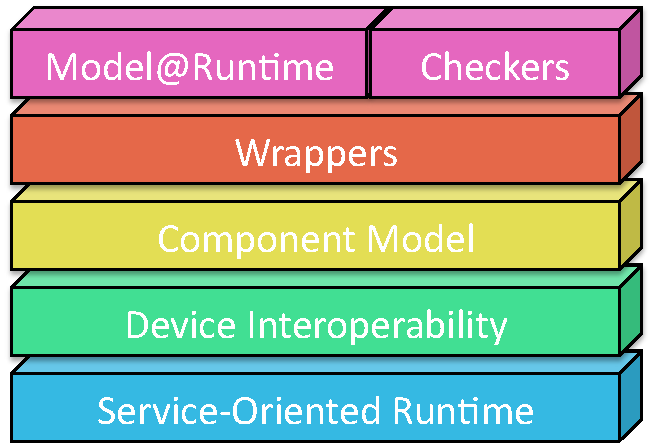
\includegraphics[width=.5\textwidth]{part2/pics/layers/AllBig.pdf}
  \caption{Overview of the EnTiMid layers}
  \label{fig:allLayersBig}
\end{figure}


{\bf Device Interoperability} addresses the mandatory need for {\it interoperability}. It is responsible for communication with real devices and their representatives in the {\it Component Model}.\\

The {\bf Component Model} involves structures and methods, to handle abstract representations of real devices. It provides a unified description of available ports, parameters, and any other useful information for the {\it Model@Runtime} layer to work in good conditions. It enables the creation of tools to cope with variability, interoperability and safety concerns.\\

The {\bf Model@Runtime \& Checkers} layer concerns the necessary tools to ease the management of the system. The implementation specificities of components are invisible at this level, thanks to the {\it Component Model} layer. Simulations and checks can be safely performed at this level of abstraction, with no consequences on the running application. Model@Runtime enables the management of the system while running, and helps in dealing with variability management. Checkers offers tools for validation and improvements for the safety of the solution.\\

The {\bf Wrappers} layer takes responsibility for publishing the devices present in the system, on application level networks. This ability opens our solution to existing and future, protocols and evolutions. Often too heavy to be embedded, this layer offers the devices, for free, an access through application level protocols.\\

The {\bf Service Oriented Runtime} completes the contribution, by offering an execution environment for the new component model. It brings "life to the {\it Model@Runtime}" by providing the support for dynamic {\it adaptations} and {\it evolutions} while running.\\

Each level participates in meeting the requirements identified in chapter~\ref{ch:requirements}. Table~\ref{table:layer_req} shows what concern is addressed by each layer. Separately, each layer does not satisfy all needs, but their collaboration does.\\

\begin{table}[h!]
\begin{tabular}{m{.20\textwidth}| >{\centering\arraybackslash}m{.12\textwidth}| >{\centering\arraybackslash}m{.07\textwidth}| >{\centering\arraybackslash}m{.09\textwidth}| >{\centering\arraybackslash}m{.08\textwidth}| >{\centering}m{.11\textwidth}| >{\centering\arraybackslash}m{.12\textwidth}|}
 {\it Takes part in}& {\tiny Interoperability} & {\tiny Openness} & {\tiny Adaptation} & {\tiny Evolution} & {\tiny Variability Management} & {\tiny Safety \& Security}\\
 \hline\hline
 {\small Model@Runtime} & & & + & + & + & + \\
  \hline
 {\small Wrappers} & & + &  & + &  & \\
  \hline
 {\small Component Model} & + & & + & + & & \\
  \hline
 {\small Device Interop.} & + & & & & & \\
  \hline
 {\small Service-Oriented Runtime} & & & + & + & &\\
 \hline
\end{tabular}
 \caption{Mapping layers to requirements}
 \label{table:layer_req}
\end{table}

%\begin{wrapfigure}{r}{40mm}
%  \vspace{-4mm}
%  
\includegraphics[width=40mm]{part2/pics/entimidLogo.png}
%  %\vspace{-5cm}
%\end{wrapfigure}

\par This contribution has been implemented. The runtime, called \enti{}, has been developed on top of an OSGi platform. By the way, \enti{} is a compound word from the Breton "En Ti", which means "In house", and "Mid", for Middleware. It is thus the middleware in the house. The component model has been developed using classical modeling techniques. Tools have been created to enable all functionalities.\\
Chapter~\ref{ch:detailsStrata} details each layer of this contribution.


\chapter{Details on strata}
\label{ch:detailsStrata}


Like a geologist, this chapter dissects the contribution layer by layer. For each stratum composing the proposal, a section gives details on the roles taken on by the layer, its achievements, and its interactions with other strata.\\

The first section starts with the description of the Device Interoperability layer, which takes an essential role in the contribution since it enables heterogeneous connections. Section~\ref{sec:componentModel} then details the different concepts present in the component model, their interactions, and describes how the synchronization between component implementations and models is guaranteed. Section~\ref{sec:martAndReasoning} explains how the Model@Runtime and Reasoning layer takes advantage of the component model to offer a great flexibility and multiple points for checking the conformance. The runtime environment chose is briefly presented is section~\ref{sec:soaruntime}, while section~\ref{sec:wrappers} introduces the Wrappers layer.

\section{Device Interoperability}

\begin{wrapfigure}{r}{60mm}
  \vspace{-5mm}
  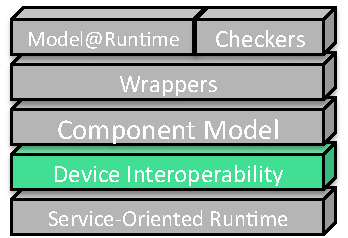
\includegraphics[width=60mm]{part2/pics/layers/DevicesInterop.pdf}
%  \caption{Interoperability Layer}
%  \label{fig:interopLayer}
  \vspace{-5mm}
\end{wrapfigure}

The Device Interoperability layer is probably the most important layer of the approach, since it answers the first requirement. Variability management, adaptations, or evolutions, would be compromised if only two devices were not able to communicate. Interoperability of devices is a central concern. It offers a foundation on which other layers can be built. This section presents how this interoperability has been realized.\\

In the domain of home automation, communication protocols used by manufacturers and their devices are not compatible. This incompatibility makes any direct interaction of devices coming from different brands impossible. To overcome this barrier, some manufacturers have worked in a consortium to define a unique communication protocol for their respective products to be compatible. However, some of their products code Boolean values on a single bit, while others code it on a byte. Again, two products may not be operable with each other.\\
In~\cite{Bromberg:2009} Bromberg et al. propose to automatically generate gateways between protocols, in order to address this issue. But building protocol-to-protocol translators solves the problem only partially, because the number of translators exponentially explodes with the number of protocols. Nevertheless, this proposition seems very interesting for an automatic generation of translators, from specific protocols to a higher-level of abstraction model.

\subsection{Use of drivers}
\label{subsec:useOfDrivers}
To realize this abstraction, drivers have been developed. A driver makes the link between real world devices and their virtual representation in a software system. Thus, they take on two responsibilities. In one way, they convert from vendor-specific communication messages to actions on their virtual representative. Naturally, they translate in the other way, actions on virtual elements into vendor-specific messages. \\
Secondly, drivers provide the virtual structures for each product they are able to interact with. All implementations specific to a given manufacturer are thus contained in drivers, or separate libraries. This makes the core system completely independent from devices' implementation specificities.\\

This independence implies the creation of a common structure, for the system to be able to properly handle devices in a good abstraction level.

\subsection{Functional interfaces}

This common structure may take the form of a set of programming interfaces. Each interface could specify a set of methods for a specific functionality. Then, drivers just have to provide objects, decorated with some interfaces, selected according to the abilities of each device. This set of programming interfaces has been created. A survey of devices functions has allowed us to extract the minimum set of common methods for each function as presented in figure~\ref{fig:interfaces} for instance. Once the set is defined, a library containing all interfaces was compiled and included in the framework.\\
\begin{figure}[h!]
\centering
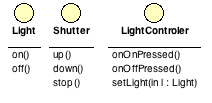
\includegraphics{part2/pics/FunctionalInterfaces.png}
\caption{Functional Interfaces}
\label{fig:interfaces}
\end{figure}
The first experiments were promising. Interoperability was almost solved, but several drawbacks were rapidly identified while using this approach in real use cases. The set of interfaces is only extensible by augmentation of the framework. The development of a device driver could have fail because the required function interface was not available in the library. Moreover, direct method calls are not appropriate if the system has to consider a dynamic environment, in which objects unpredictably appear and disappear. In this case, object-oriented development using synchronous method calls becomes quite hazardous. Finally, if for any reason a component implementing the {\it LightControler} interface has to be plugged into a shutter, the operation is simply not feasible without an ad-hoc adapter (illustrated in figure~\ref{fig:interfaces}). Interoperability was not solved.\\


\subsection{Event-based approach}

Real-life events can occur in any order, at any time, in any context. Moreover, devices are more and more mobile and can dynamically join or quit the system. In order to address this dynamicity, we made use of event-based mechanisms. \gls{mom} offers a simple, and efficient means of communications, using the publish/subscribe principle. Event consumers subscribe to a topic they are interested in, and event producers just have to publish on the right topic. Thus, producers do not care about the presence of consumers.\\
To be able to use this approach, physical devices have been considered from two perspectives. {\it Sensors} sense real life and human actions. Their role is to feed the system with events coming from real life. They are producers of events. Consuming these events, {\it Actuators} act on real life, using real-life equipment. They carry out orders such as switching on the lights, or opening or closing the shutters. 
Components are not limited to a unique role, and can both consume and produce events.\\

{\bf Actuators} propose two main methods. {\it getAvailableActions()} returns a list of actions that can be carried out on the device. If a light can answer [{\it on,off}], a shutter could answer [{\it up,down,stop}]. For each action, actuators wait for messages on a specific topic. For a sensor to ask for an action to be realized, it must know the corresponding topic. {\it getTopicFor(String action)} aims at providing the topic and the parameters that can be accepted for a given action in form of a {\it Message}.\\

{\bf Sensors} maintain a list of messages for each event they sense. An On/Off switch maintains two lists of messages: one for each action. The messages stored also embed the topic on which they have to be published, for the action to be carried out. When an action is sensed, each message stored for this action is sent on its topic.


\subsection{Example}

For instance, figure~\ref{fig:seqDiagConfMom} shows the configuration phase for the connection of a switch and a light. The \textit{Configurator} retrieves the message to be sent to switch on the light. This message is added to the list of the "on" sensed value of the switch. Later, when the "on" button is pressed, all messages stocked in the list are sent. When an actuator recognizes its "on action message", it forwards the order to the real light.\\

\begin{figure}
\centering
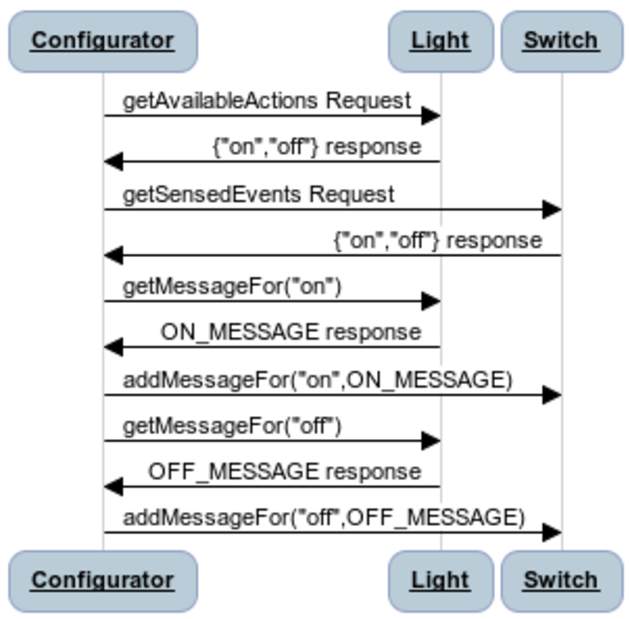
\includegraphics[width=.5\textwidth]{part2/pics/SequenceDiagram.pdf}
\caption{Configuration Phase}
\label{fig:seqDiagConfMom}
\end{figure}

This mechanism allowed us to eliminate asynchronous aspects. It also allowed any sensor to control any actuator, since they do not have to know each other to be able to work together. The action carried out and the value sensed do not have to necessarily be the same. Thanks to the mechanism of messages, it is possible to send the "on" message to the light when "down" is sensed by a shutter command.\\

\begin{figure}
\centering
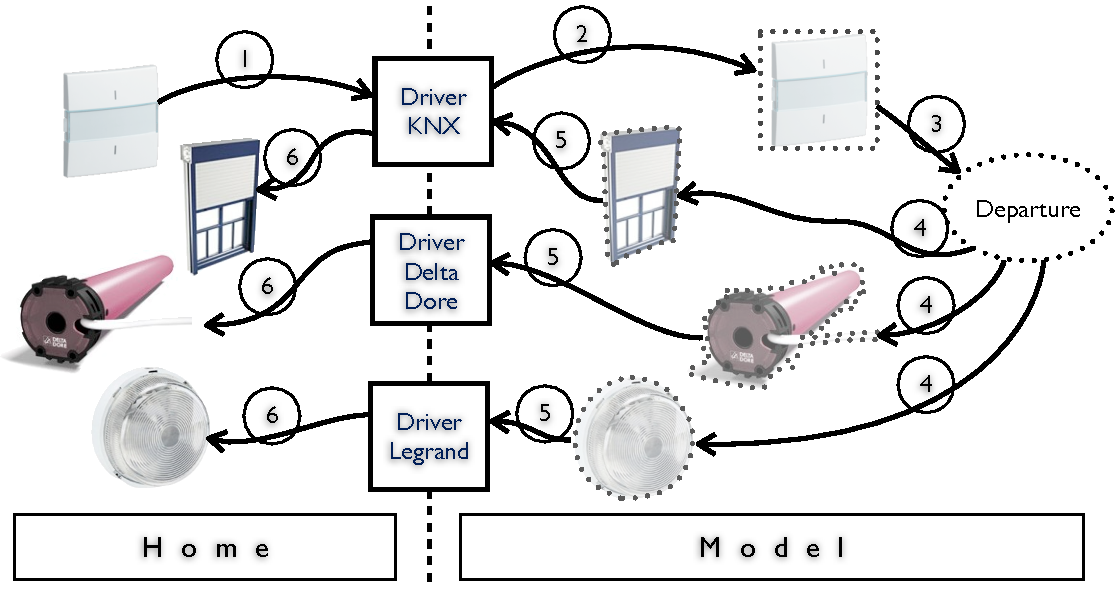
\includegraphics[width=.8\textwidth]{part2/pics/InteropExample}
\caption{Example of Interoperability}
\label{fig:interopExample}
\end{figure}


Let us consider a home with a switch to trigger a departure scenario, operable on the KNX network. This scenario switches off all lights and closes shutters. In the considered example, there are only two shutters and one light. The first shutter was motorized when the house was built and works on a KNX network. The second shutter was added afterwards and as the owners did not want to make holes in the walls, they chose a shutter engine communicating with the command by radio frequencies. Lastly, lights are controlled by Legrand equipment. All these elements are visible on the left of figure~\ref{fig:interopExample}.\\
The interoperation of all these elements is described in the case of a departure scenario activation. Numbers on the figure present the sequence of actions.\\
{\bf 1-} An inhabitant presses the button. This action is sensed, and generates a message on the KNX network.\\
{\bf 2-} This message is read by the driver and translated into a message for the EnTiMid system.\\
{\bf 3-} The driver then selects the virtual representation of the device responsible for the message and activates the sending of stored messages.\\
{\bf 4-} Its activation causes all connected elements to be activated in parallel.\\
{\bf 5-} On receiving the message, each model representative of a real product asks its driver to send an order to the real product.\\
{\bf 6-} The driver executes the query and sends the order.\\
In this example, various devices with various actions are connected together. A switch that senses a {\it departure} is connected to two {\it down} actions on two different components and one {\it off} port. Interactions between components are possible thanks to the exchange of messages.\\

\subsection{Threat to validity}
Interoperability was tested and validated with a restricted set of devices. Since the main goal of this thesis is not about making any device interoperable, the study was conducted with a set of representative technologies mixing different communications media, different appliances and multiple manufacturers, in order to prove the feasibility. 

\subsection{Summary}

The {\it Device Interoperability} layer enables products from any manufacturer to work with any other product, in any imaginable way, by just implementing a driver. The use of this method is however limited by the non-availability of action lists at design time. Each device provides information about the actions it supports, but a method has to be called. Since method calls cannot be done at design time, the only way to obtain available actions is to go and seek them in the implementation code.\\
The sequence diagram, presented in figure~\ref{fig:seqDiagConfMom}, describes a part of the work that a piece of program has to execute to set up the application's behavior. The sequence cannot be implemented definitively, since the application may have to be adapted and to evolve while running. The configuration has to be expressed another way, to be modifiable, and to ease the reading and understanding of the behavior.\\

Both of these issues require a tool. It has to be able to provide information about the devices at design time, and it has to support and help device assembly design. This tool, a new component model, is made available by the {\it Component Model} layer.

\newpage
\section{Component Model}
\label{sec:componentModel}
\begin{wrapfigure}{r}{60mm}
  \vspace{-8mm}
  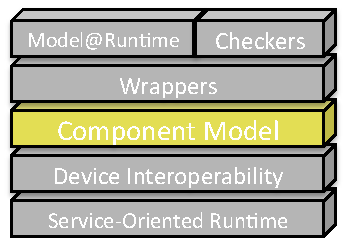
\includegraphics[width=60mm]{part2/pics/layers/ComponentModel.pdf}
%  \caption{Component Layer}
%  \label{fig:componentLayer}
  \vspace{-8mm}
\end{wrapfigure}

On top of the {\it Device Interoperability} layer, a tool is required to make devices' abilities and their interactions explicit. This tool has to take into account the sporadic apparition of devices. Component models have been identified as good candidates to take on this role. They are very good representatives of real life devices, since they can use or provide services. Their interfaces(as lists of actions used or provided) are made explicit. Their life cycle is very helpful to catch the dynamicity of the devices' presence. Finally, the concept of components in software engineering is very close to electronic components.
%It makes it easy to understand and manipulate for anyone familiar with electronic components.
Device manufacturers and software developers have here a common discussion base, a common language.\\
As presented in the state of the art, component models are often too strict and prevent components from connecting with non-identical interfaces. This restriction could compromise the interoperability gained by the {\it Device Interoperability} level, whereas this layer just aims to simplify the configuration and management.\\

This section is organized as follows: section~\ref{subsec:makeSoftCloserToElec} emphazes the relation between the proposed component model and electronic components. This relation is illustrated in section~\ref{subsec:compoModConcreteExample}. The mechanisms responsible for the synchronization of model and code are presented in section~\ref{subsec:compModBinToModel}. Lastly, section~\ref{subsec:compModLinkWithInterop} describes how the {\it Device Interoperability} integrates with this layer.


\subsection{Making software components closer to electronic components}
\label{subsec:makeSoftCloserToElec}

When talking about components, electronic ones are probably the first kind of component to come to mind for a lot of people. An electronic component, as shown in the bottom left part of figure~\ref{fig:elecDataSheet}, is a black box surrounded by pins. The shape of the pins is standard and allows components to be connected to any board. Obviously, neither the pins nor the board have the ability to refuse the connection of two components. This absence of constraints allows electronic components to be used in a large variety of contexts. They can be connected to a multitude of other components to create appliances. This is the perfect description of the behavior required for a software component.\\
Nevertheless, software components' ports are generally specialized by a programming interface (API). Thus, unlike electronic components' pins, their shapes are not standard. The goal of this specialization is to ensure the alignment of services. However, this is too strong a limitation in our context.\\

In electronics, components admit only three kinds of ports (pins).\\
{\bf Input Ports} collect all necessary information from the outside, for the component to do its job. At the same time, they can trigger the execution of an associated task. Typical examples are the \textit{A} and \textit{B} input values of a comparator.\\
{\bf Output Ports} release the data resulting in the execution of a task. The \textit{C} result value of a comparator and the tick of a timer, are two illustrations of this kind of port.\\
{\bf Parameter Ports} are used to set specific values for an instance. They specialize the behavior of the instance for a specific context. An example could be the \textit{clock} port of a microchip, which can be set to several frequencies according to the application it is involved in.\\

\begin{figure}
\centering
	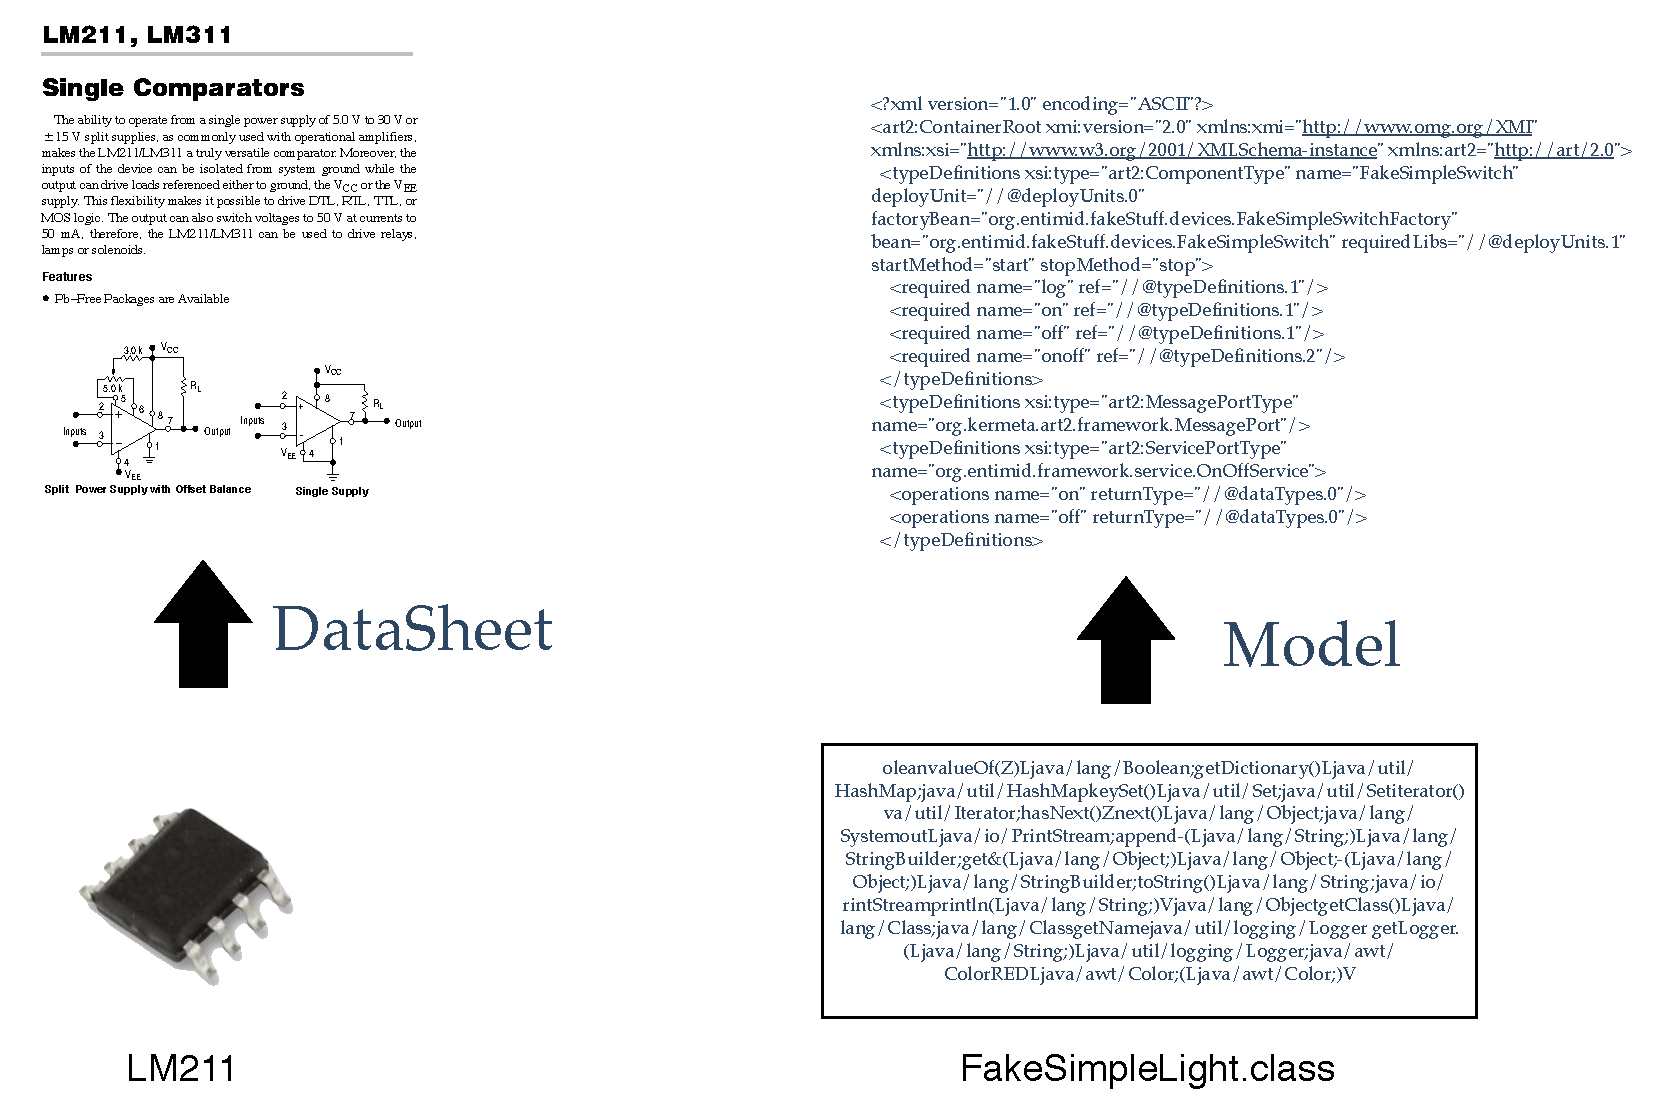
\includegraphics[width=.9\textwidth]{part2/pics/DataSheet.pdf}
	\caption{Electronic Parallel: Datasheets}
 	\label{fig:elecDataSheet}
\end{figure}

The component model created was strongly inspired by electronic components. Indeed, {\it InputPorts} and {\it OutputPorts} have been implemented as presented in figure~\ref{fig:component_type:logical}. They have been divided into \textit{synchronous} and \textit{asynchronous} kinds, to handle both object-based method call handling, and message-based communications between components.\\

\subsection{Meta-Model description}
 
This section details the elements of the component model, presented in~\ref{fig:component_type:model}.\\

{\bf ComponentType}\\

The {\it ComponentType} meta-class carries the component description specification. Ports of the component are describes in collections; provided for input ports, required for output ports. The component type also contains a dictionary which declares parameters, and their default values, that can be specialized for each component instance.\\

{\bf Ports}\\

To keep close to existing component models and promote compatibility, the component model makes use of classical terms in its implementation. As a consequence, {\it InputPorts} are implemented as {\it provided} ports and {\it OutputPorts} as {\it required} ports, as shown in figure~\ref{fig:component_type:model}. For their part {\it ParameterPorts} have been implemented as <key,value> dictionaries.\\

\paragraph{ParameterPorts}
This kind of port is used to specialize component behavior. For example, the \textit{Timer} component uses a \textit{delay} parameter that represents the amount of time to be spent before the time-out occurs. A component can have multiple parameters. They are uniquely named in the component's scope, and can be optional or mandatory. All parameters a component admits are listed in a dictionary at model level.
At runtime, each parameter port is instantiated as a setter method, which only admits a dictionary as parameter. Indeed, each parameter port has its own setter method. Both keys and value types are Strings. This ensures the transmission of parameters in a unified way. Each component is responsible for the conversion from the String to the real type of its parameters.\\
To keep the link with electronic components, the method is the pin, and the dictionary describes the shape of the signal to be sent (voltage, intensity, shape of the signal).

\begin{figure}
\begin{center}
\subfloat[Component Type]{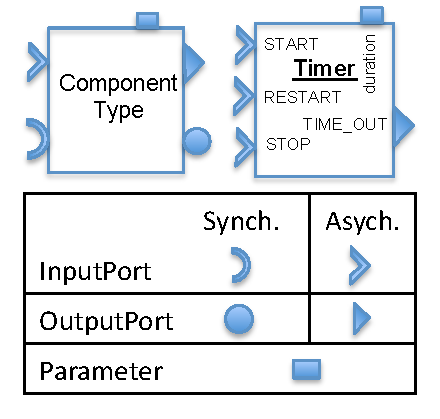
\includegraphics[width=.3\textwidth]{part2/pics/component_type3}\label{fig:component_type:logical}}
\hspace{3mm}
\subfloat[Meta-Model Excerpt]{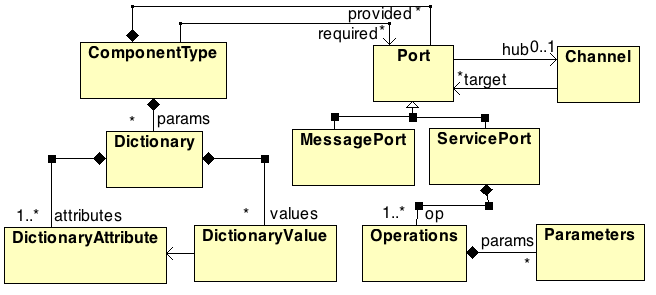
\includegraphics[width=.65\textwidth]{part2/pics/meta-model.png}\label{fig:component_type:model}}
\end{center}
\caption{Extraction of a part of the component model architecture}
\label{fig:component_type}
\end{figure}

\paragraph{InputPorts}
A component can provide several facilities to other components. This is illustrated by the \textit{Timer} on figure~\ref{fig:component_type:logical} which offers start, stop, and restart actions. In classical software component models, the timer component would have provided a single synchronous port with the three start, stop, and restart methods. These methods would have been defined in the StartStopRestart API.\\
Synchronous ports (also called ServicePorts in the model) act the usual way: they are typed by an API, and are based on method calls. Thus, our component model is able to support the common software-component behavior. However, this is not the way of designing components that we encourage.
Indeed, the API is typed by the programming language type system, and this typing may prevent components from being connected because of a mismatch. We want to elevate the typing from the language to the model, and resolve the typing at a higher-level of abstraction.\\
Asynchronous ports, handled as \textit{MessagePorts} in the component model (fig~\ref{fig:component_type:model}), are much more interesting for the promotion of component connectivity. Each method/action a component offers is accessible through a dedicated port. Each port is uniquely named in the scope of the component. In the same way, electronic components have one pin for each action and actions are triggered when the value changes from 0 to 1 for instance, on the corresponding pin.\\
To mimic this behavior, all asynchronous {\it InputPorts} are implemented as a {\it Command} design pattern. They have a unique method {\it public void process(Dictionary<String, String>)}. The uniqueness and standardization of the method are mandatory to ensure the connectivity.\\
Just as an electronic component, actions in our component model can have parameters. Coded in the shape of the input signal passed through an input pin in electronics, our \textit{InputPorts} admit a dictionary of <key, value> parameters. Like ParameterPorts, this dictionary only allows pairs of Strings. These values are specific to each execution and may change form one call to another. In figure~\ref{fig:component_type}, \textit{START}, \textit{STOP} and \textit{RESTART} are all InputPorts. The parameters used on the start or restart activation are transferred through the \textit{TIME\_OUT} OutputPort to the connected component.\\

\begin{figure}
\centering
	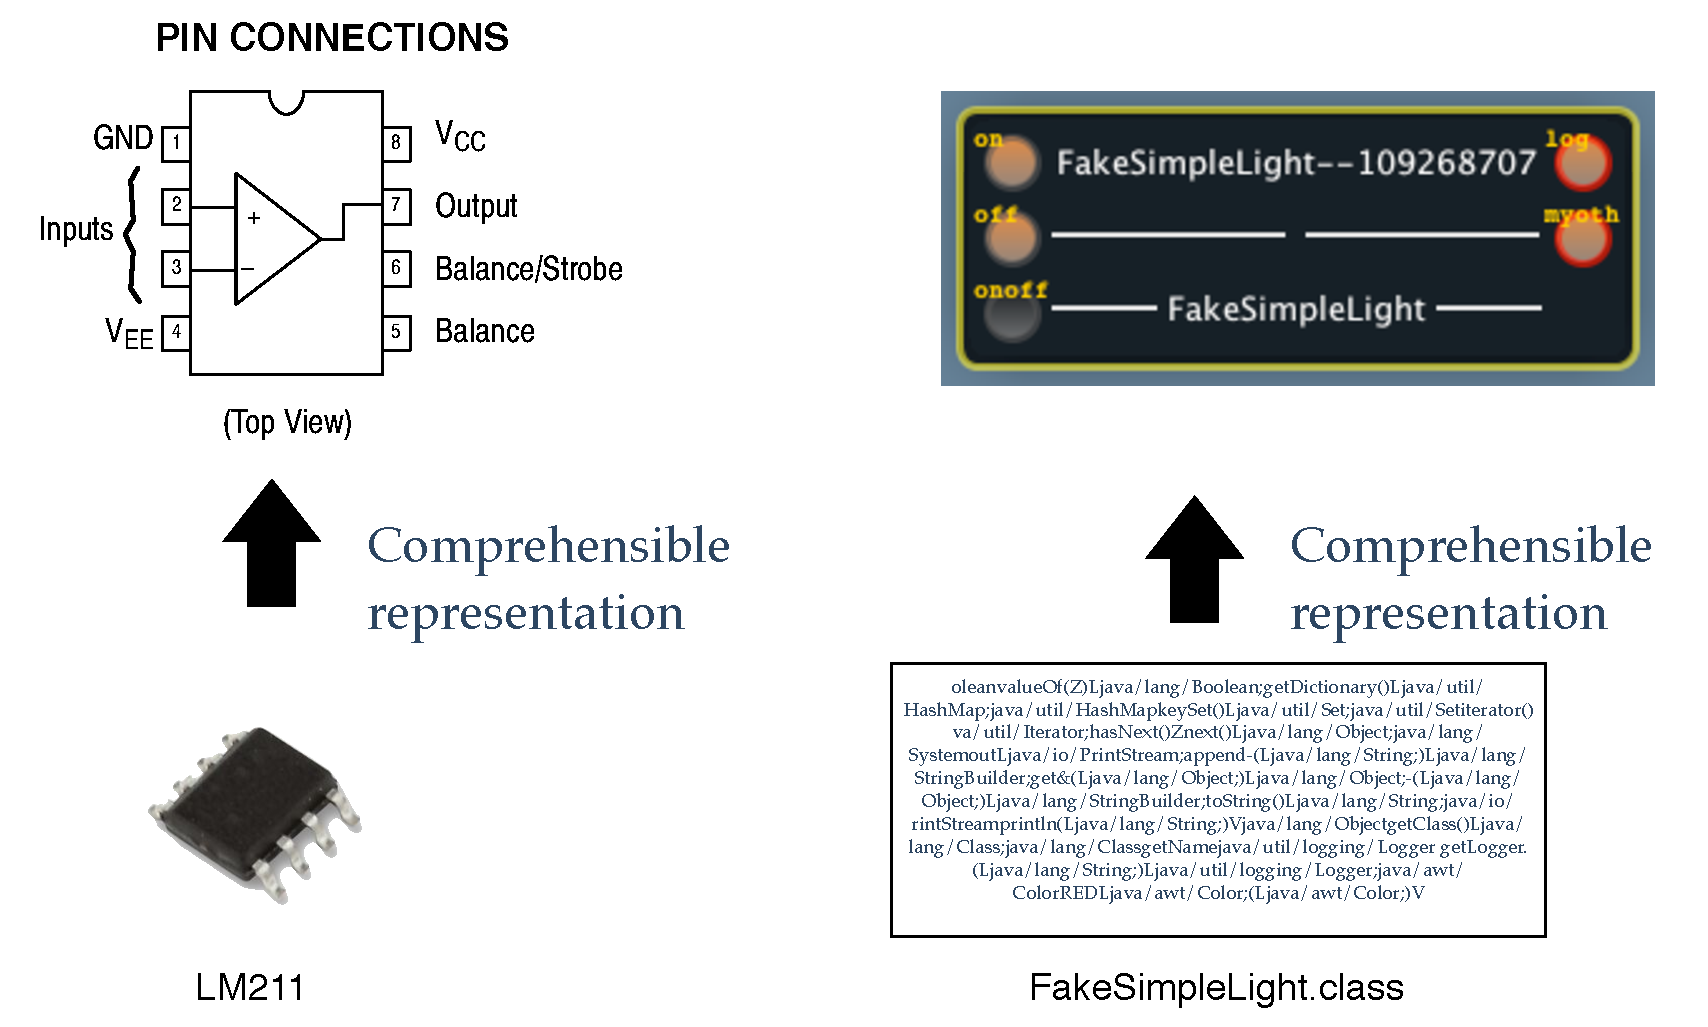
\includegraphics[width=.8\textwidth]{part2/pics/ComponentView.pdf}
	\caption{Electronic Parallel: Components}
  	\label{fig:elecComponent}
\end{figure}


\paragraph{OutputPorts}
The main role of an OutputPort is to forward or release information. For instance, in figure~\ref{fig:component_type:logical} when the timer delay is over, the \textit{TIME\_OUT} port is activated and thus the connected InputPort (if any) also is. In case the activated \textit{InputPort} is synchronous, the result of its activation is returned by the called method. This is a blocking behavior, and may not be adapted to events coming from real life. If the activated port is a MessagePort, the result of its execution (if any) is given though a dedicated \textit{OutputPort}.\\


All this results in a parallel between electronic and software components as shown by figure~\ref{fig:elecComponent}. Input(provided) ports are displayed on the left side, and Output (required) ports are on the right.\\

{\bf Channel}\\

A Channel connects two or several ports. Channels can be of different types, and are instantiated just as components are. Channels are providing communications to components. These communications can be realized with several protocols, politics and media. According to the situation, one can make use of a channel that sends messages in sequence, or of one sending in parallel. Channels can create the link using TCP or UDP sockets, RS232 serial connection, or a REST request. Channels are handling the communication semantic and method between components.\\
Being defined outside the component, developers can make no assumption about the media or protocol that will be used, or the kind of component on the other side. This enforces the development of well defined standalone components and promote their reuse.\\

{\bf Service Ports}\\

Service ports come with the description of their operations (name, returned value) and a description of the operations' parameters (names and types). These information are used by channels, modeling tools and runtime platforms. Channels can play a role of mediation between not exactly aligned services descriptions. Modeling tools use these description to perform checks on component assemblies and authorize au not components' connections. Finally, runtime platforms can check the alignment, and may refuse any connection that violates a pre-defined connection rule.\\
These checks are detailed in section~\ref{subsec:check_to_validate}.

\subsection{Concrete example}
\label{subsec:compoModConcreteExample}
This example shows how a real product is implemented in this component model. The RMG4S, on the left side of figure~\ref{fig:rmg4s}, is a KNX product by Theben\footnote{http://www.theben.de/en}. This product can control up to four 230V lights or sockets. Its virtual representative has 8 message input ports, two (i.e.: on, off) for each controllable element. When a physical event changes the state of an output of the product (somebody switches on the light using the dedicated switch), the state is propagated to any connected device, through the corresponding port of the component.\\
In addition, a {\it KnxEnv} input port allows the driver to circulate real-life events. On the other hand, an output port {\it KnxNetwork} is used to send events from the model element to the real product through the driver. The last output port is a logging port.\\
Thus, to switch on the light that is physically connected to the first module of this product, one just has to activate the {\it m1\_on} port. The component then asks its driver to send a message to the real device to make it power up its first module.\\
On the other hand, when the state of a module is physically changed, a message is sent from the driver to the component. The component then activates the {\it m1\_state} (for instance), to inform any connected component about the change.\\
If the application proposes a graphical user interface, the {\it on} (resp. {\it off}) port of the component is activated when the user presses the graphical button. On activation, the driver sends the order to the real product, which reacts and sends information about its state change. The driver catches the information, and sends it to the graphical interface for update, through the dedicated output port of the component.\\ 

\begin{figure}
\centering
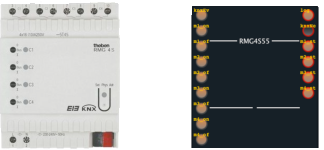
\includegraphics[width=.7\textwidth]{part2/pics/RMG4sModel}
\caption{Example Model}
\label{fig:rmg4s}
\end{figure}

The component model makes our software equivalent to electronic components \textit{DataSheets}. Assembly constraints, mandatory parameters on ports, component behavior, and many other pieces of information on components can be expressed in the model. This abstract description of the component has no effect on the runtime implementation (just as \textit{DataSheets} have no effect on black-box components by the way).\\


\subsection{Implementation and Model Relationship}
\label{subsec:compModBinToModel}
\begin{figure}
\centering
\begin{lstlisting}[caption=Java class POJO annotation,label=fig:jcPOJOannot,basicstyle=\scriptsize\ttfamily,tabsize=2 ]
@Provides({
    @ProvidedPort(name = "start", type = PortType.MESSAGE),
    @ProvidedPort(name = "stop", type = PortType.MESSAGE),
    @ProvidedPort(name = "restart", type = PortType.MESSAGE) })
@Requires({
    @RequiredPort(name = "timeOut", type = PortType.MESSAGE),
    @RequiredPort(name = "logger", type = PortType.MESSAGE) })
@DictionaryType({
    @DictionaryAttribute(name = "time", default="3000") })
@Library(name="EnTiMid - Framework")
@ComponentType
public class Timer extends AbstractComponent {

	private TimerThread timer;
	private long time = 3000;  // default value

	public Timer() {}
	public Timer(final long time) { this();  this.time = time; }

	public long getTimeOut() { return this.time; }    
	public void setTimeOut(long value) {
		if (value > 0) { this.time = value; }
	}

	@Port(name = "stop")
	public void stopTimer(Message m) {
		if (timer != null) { timer.reset(); }
		getPortByName("logger", MessagePort.class).process("Timer("+time+")::STOP");
	}

	@Ports({ @Port(name = "restart"), @Port(name = "start") })
	public void restartTimer(Message m) {
		if (timer != null) { timer.reset(); }
		timer = new TimerThread();
		timer.start();
		getPortByName("logger", MessagePort.class)
			.process("Timer("+time+")::STARTED");
	}

	@Start
	public void start() {
		time = Integer.valueOf(getDictionary().getValue("time")).intValue();
		getPortByName("logger", MessagePort.class).process("Start Timer");
	}

	@Stop
	public void stop() {
		getPortByName("logger", MessagePort.class).process("Stop Timer");
	}

	@Update
	public void kevUpdate() {
		time = Integer.valueOf(getDictionary().getValue("time")).intValue();
		getPortByName("logger", MessagePort.class).process("Updating Timer");
	}
\end{lstlisting} 
\end{figure}


The development of a component (i.e.: a virtual representative of a physical device) can be achieved in two ways. According to its preferences, the developer can make the model of what he wants, and ask for code generation. This approach is called {\it Model First}. The model can also be extracted directly from annotations decorating the implementation code made by the developer. This is called {\it Code First}. The code first approach differs from a reverse engineering approach, in the sense that the model is extracted from annotations in the code, and not from the implementation code itself. These two approaches are not exclusive. The model of a component can evolve, therefore impacting its implementation. Respectively, if a change is made to the code, it has to be reproduced at the modeling level. In other words, the consistency between implementation and model has to be guaranteed.\\

To illustrate the description, listing~\ref{fig:jcPOJOannot} shows the complete implementation class of a {\it Timer} component. This listing is organized as follows: on the first lines are annotations on the class that describe the component shape. Just after, the class definition comes with private attributes, object builders, then getters and setters. Next, methods render the services offered by the component. Life-cycle management methods are at the end of the class.\\

{\bf Component shape}\\
The first annotations on the class inform about the {\it Input}, {\it Output} and {\it Parameter} ports. As explained in section~\ref{subsec:makeSoftCloserToElec}, {\it InputPorts} are implemented as {\it provided ports}. Common actions that can be carried out on a timer (start, stop, restart) are listed under these terms.\\
This {\it Timer} implementation offers two outputs, visible as {\it Required Ports}. A {\it log} port, which sends information about the internal behavior of the component, and a {\it time\_out} port activated when the countdown ends.\\
The Timer admits a parameter. This parameter sets the delay between the start and the activation of the time\_out port. This parameter appears in a dictionary.\\
The {\it @Library} indicates that the component is part of the virtual library of components called "EnTiMid - Framework". In edition tools, all components of the same library are presented under the same package of components. A library of components can be defined using several deployment units.\\
The last annotation simply tags the class as a component type implementation. This annotation is mandatory for the compilation tools to consider the class as a component type.\\

{\bf Port mappings}\\
Once described, input ports have to be linked to the method implementing the action. In the example, one may remark that a port can be bound to at most one method, but a method can be reached from several ports. Indeed, the behavior of a {\it start} and a {\it restart} of a timer are implemented the same way. Classical solutions could have been to remove one action or to copy-paste the method. From a user perspective (sect.~\ref{subsec:keepUserInMind}), a Timer should be able to be started and restarted which implies not to removing the port. Thanks to this multiple mapping, the user will be satisfied with no redundancy of code.\\
Moreover, the transfer of the annotation from one method to another, changes the method called when a port is activated. This change is completely transparent for assemblies already using the component, since the annotation is not modified. This is a great ability that enables changes in the implementation and method names, with no change in the component interface.\\
Finally, a component can offer the same service through both {\it Service} and {\it Message} port. Using the same mechanism, the same method can be called in both cases.\\

{\bf Life cycle}\\
{\it Start} and {\it Stop} life cycle methods are mandatory. They are called when an instance is started (resp. stopped). Stateless components may just ignore these methods, but stateful ones may use these to persist their state.\\
The {\it update} method is used to inform a component that one of its parameters has changed.\\

{\bf Code first}\\
Meta-information, concerning the component model, is introduced in the code using annotations. This method for including meta-information in the code has already been used in tools such as Fraclet\cite{Rouvoy:2009}. A developer familiar with the annotation set, or in charge of the migration of existing components, may directly define the model in the code.\\
As in a classical development process, the new implementation code has to be compiled to incorporate the changes in binaries. Our component model takes advantage of the compilation phase to extract the model from the annotations. A visitor goes all over compiled classes and selects the {\it @ComponentType} decorated classes. Then sub-visitors navigate into the code to create the model.\\
At the end of the compilation process, the newly-computed model is added into the compilation result. {\it i.e.} the model is included as an XML file into the {\it .jar} that results from the compilation. Model consistency with the latest code version is guaranteed this way.\\

{\bf Model First}\\
Writing component type code, plus the annotations, may become a complicated task. A non-familiarized person may experience difficulties in placing all the annotations required to describe its component.
The model-first approach aims at providing tools to graphically (or textually) describe the component first, and then ask for the implementation to be generated. This method is made available by the use of tools such as graphical \gls{dsl}, textual \gls{dsl} or generic meta-modeling languages such as Kermeta~\cite{Muller05a}. Models bring a more intuitive approach for the description of a component.\\ 
Once the developer is done with its component's model, the generation tool is activated. If the implementation class of the component does not already exist, a new file is created. This file contains the skeleton of the component implementation. Obviously, the code generation reaches its limits when the body of methods has to be created. The behavior of methods is the only part to be completed by hand by the developer. Otherwise, the class is already decorated with all annotations, and ports are mapped by default on generated methods.\\
When an implementation class already exists, the generation process is slightly more complex. In fact, a temporary model is extracted from the existing code and an \gls{ast} of the code is created. The \gls{ast} describes the code using a tree structure containing objects. Each object stands for a method, an argument, an attribute, etc. A comparison is made between the model created by the user, and the model extracted from the existing code. Each difference is analyzed, and modifications are made on the \gls{ast}. The final code is generated from the modified \gls{ast}.\\
The model-first approach helps somewhat in linking the model and the code. In any case, the resulting code still needs a developer to complete the new methods created, to remove dead code and to optimize the mappings.\\

Thanks to these mechanisms, models of components are available while the system is not running. Their conformance with the actual implementation is guaranteed by construction. This model abstraction makes it possible to create and exploit tools from \gls{mde}.\\

\subsection{Link with the interoperability layer}
\label{subsec:compModLinkWithInterop}
The actual implementation of the component model is slightly different from the view developers can have of components. The connection between two components(channel) is graphically a line linking two ports (see the top of figure~\ref{fig:linkWithInteropLayer}). The line represent a channel, dependent of the channel type selected in the library at design time. Since ports can be synchronous or asynchronous, the runtime cannot handle port connections in the same way. The activation of an output port implies different behaviors according to its type. A message output port will send messages on topics to activate the linked input ports, but a service port has to start a method call.\\

\begin{figure}[h!]
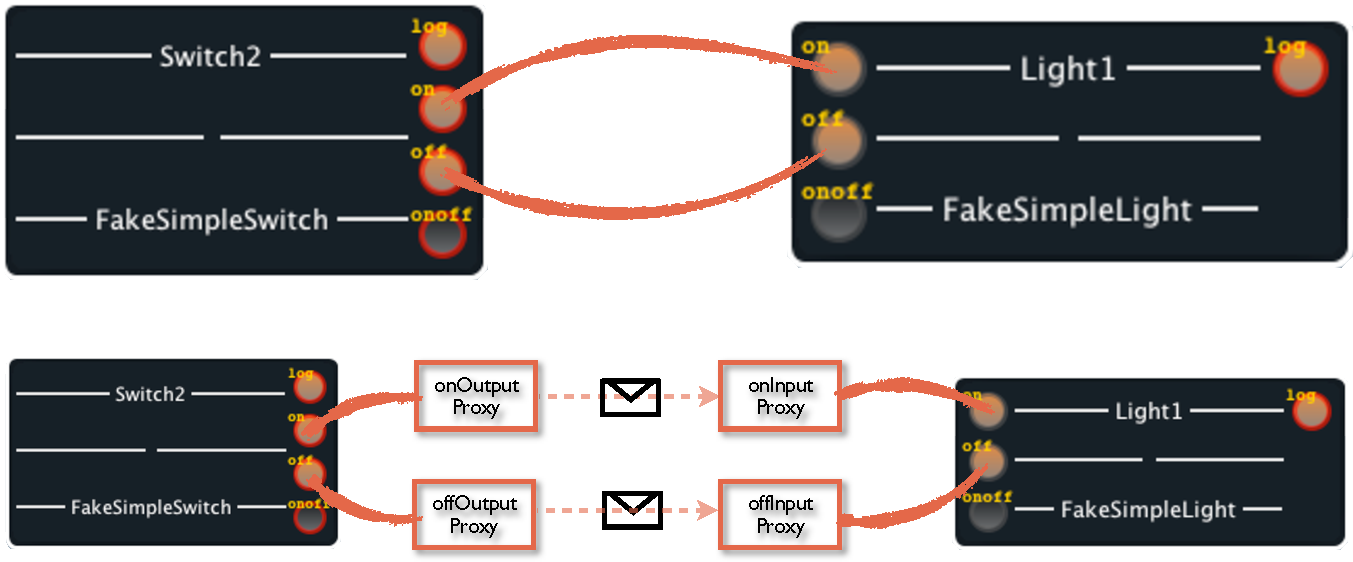
\includegraphics[width=\textwidth]{part2/pics/InteropModelLink}
\caption{Link between the interoperability layer and component connections}
\label{fig:linkWithInteropLayer}
\end{figure}

This complexity is hidden from developers in both the code and the model view of the components, by the use of proxies behind the concept of channels. At runtime, a proxy is generated for each port connected to another component's port, as illustrated in the bottom of figure~\ref{fig:linkWithInteropLayer}.\\
If the port is a message port, the proxies use messages and topics to communicate with each other. When an output port is activated, its proxy generates and sends a message on a pre-defined topic. On the other hand, a proxy listens to this topic only, and activates the input port on which it is connected when a message arrives. Activations are carried out with a {\it Command} design pattern, from the output port to activate the proxy, and from the proxy to the input port. The mechanism is thus transparent from the developer's viewpoint: an input port must provide a command pattern, an output port activates a command pattern.\\

The mechanism of proxies has also been implemented to handle the method calls of service ports. Links between components' ports are thus handled in a uniform way. The introduction of proxies makes it possible to use other means of communication (in the case of distribution issues for instance), and enables some adaptation mechanisms.\\

\subsection{Main advantage of this component model}

The main advantage of this component model is the location of the type checking. The typing of components was completely relaxed in the implementation to eliminate interoperability problems due to the implementation language type system. The typing was moved to the model level, where checks and changes in rules are made much simpler. This contribution paves the way for a pluggable type system~\cite{PapiACPE2008,Bracha:2004}.\\


\subsection{Summary}

This new component model answers the need for a tool to make the abilities of devices and their interactions explicit at design runtime. Annotations in the code is a convenient way to integrate the component model into the implementation code, and ensure the synchronization between the model and the implementation. The component model also eases the reading and understanding of an application, since all links between components are made explicit.\\

The component model imposes that the configuration is completely defined, but it is not responsible for its deployment. A gap from the component assembly to the sequence of commands to set up the application at runtime still has to be filled.\\
Since the component model has been made flexible to allow all possible connections, any connection is possible, but some may not be desirable. Just as in electronics, assemblies are constrained by components' specificities. If electronic boards allow all possible connections, components have constraints to be respected in order to assert their behavior. Assemblies have to be verified and simulated, to prevent any undesirable interactions.\\

To eliminate these two issues, the Model@Runtime approach and model checkers have been used in \enti{}. Model checkers enable verifications of component assemblies at several steps of the development, while the model@runtime takes responsibility for bridging runtime elements and the component model. These two elements of the proposal make the {\it Model@Runtime and Reasoning Engine} layer.\\


\section{Model@Runtime and Reasoning Engine}
\label{sec:martAndReasoning}

\begin{wrapfigure}{r}{60mm}
  \vspace{-5mm}
  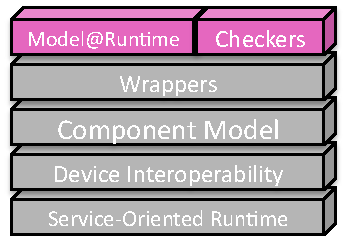
\includegraphics[width=60mm]{part2/pics/layers/MartReasoners.pdf}
%  \caption{Modeling Layer}
%  \label{fig:modelingLayer}
  \vspace{-5mm}
\end{wrapfigure}

The {\it Component Model} layer provides a level of abstraction from the implementation specificities. It offers a unified model view of components and their constraints and enables the creation of management tools. Reasoning engines, checkers, and models@runtime abilities can be used to ease the creation of component-based applications.\\
The first requirement targets the validation of assemblies, prior to their real deployment. This checking step is described in section~\ref{subsec:check_to_validate}. Section~\ref{subsec:modelatruntime} presents an overview of the use made of Models@Runtime techniques in this approach.


\subsection{Check to validate}
\label{subsec:check_to_validate}

In electronics, the components' assembly has to be approved. Its conformance in relation to components and applications-specific constraints has to be guaranteed. This validation prevents assemblies from having any computable damage. This conformance check is often carried out by simulations, based on components' specifications described in their documentation. Figure~\ref{fig:elecSimulation} shows once again the parallel between the electronic approach and ours, where electronic simulations are replaced by model checking in our context.\\

\begin{figure}[h!]
	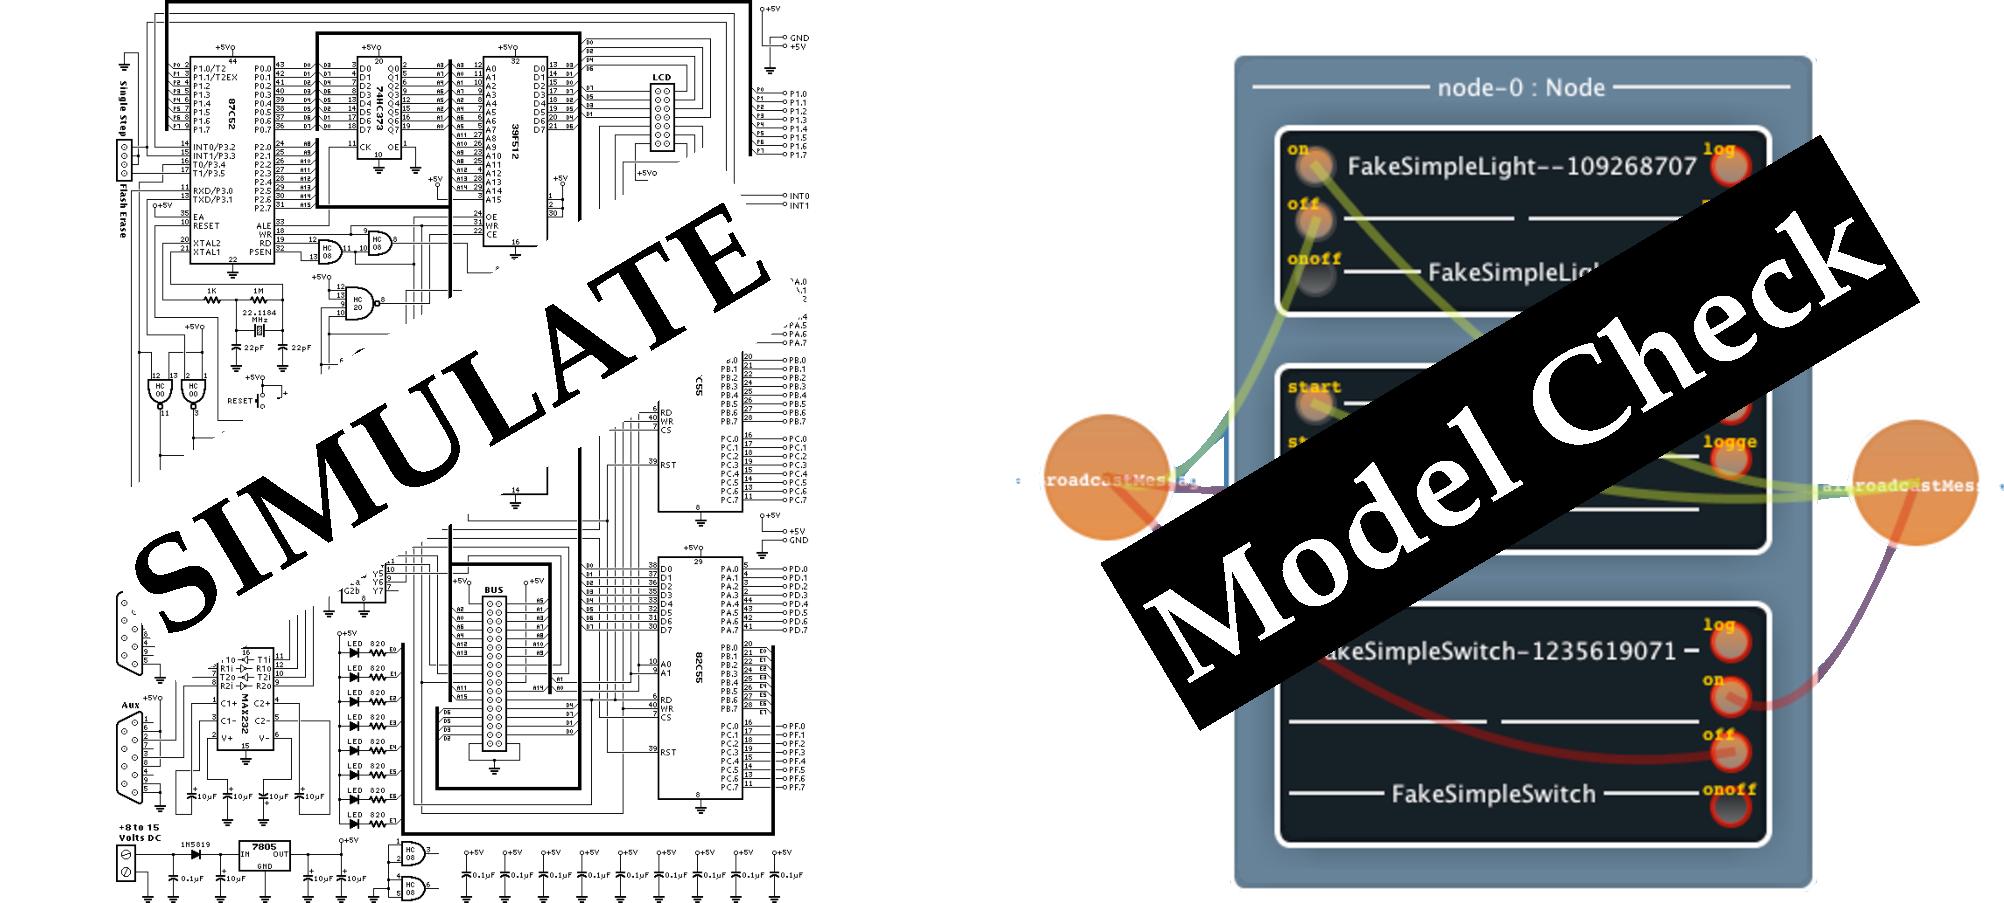
\includegraphics[width=\textwidth]{part2/pics/ModelCheck.pdf}
	\caption{Electronic Parallel: Simulation}
  	\label{fig:elecSimulation}
\end{figure}

In a classical software engineering process, conformance checking is done at 1) design time by the developer, 2) compilation time automatically, and 3) by running tests on the application built. The modeling approach offers a way to perform more precise checks, targeting more specific concerns, at several moments between the design and deployment phases. Figure~\ref{fig:checkPoints} displays the different moments where checks can be performed and illustrates what can be checked at each moment. These steps are detailed in the following paragraphs.
\begin{figure}
\centering
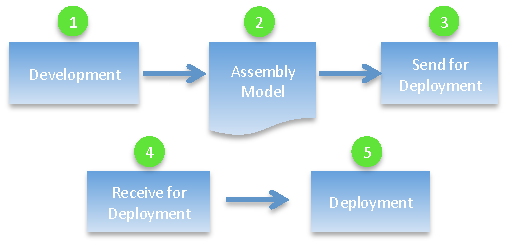
\includegraphics[width=.8\textwidth]{part2/pics/CheckPositions.pdf}
\caption{Checkpoint positions in the assembly deployment chain}
\label{fig:checkPoints}
\end{figure}


\begin{enumerate}
\item {\bf Developer's actions}\\
The assembly tool can monitor developers' actions. During the design phase, checkers can verify that only authorized operations are executed by the developer. When an inappropriate action is carried out, the triggering of warnings and errors can improve the development process. Thanks to this information, developers can immediately correct their code and learn from their mistakes. The earlier errors are detected and corrections made, the more the impact on the global solution is reduced. Also, developers' profiles could be created and associated with different checking policies according to the developers' expertise. This provides a fine-grained checking process for the design of applications.

\begin{figure}
\centering
\begin{lstlisting}[caption=Example checking developpers' actions,label=fig:checkDevAct,basicstyle=\scriptsize\ttfamily,tabsize=1 ]
def checkBindingsHomogeneity(model:ContainerRoot)
	: java.util.List[CheckerViolation]={
 model.getChannels.foreach { channel =>
  val bindingsOnChannel = model.getBindings.filter(mb =>
   mb.getChannels.equals(channel)
  )
  var synchBindings: List[Bindings] = List()
  var asynchBindings: List[Bindings] = List()
  bindingsOnChannel.foreach { binding =>
   if (binding.getPort.getPortTypeRef.getRef.isInstanceOf[ServicePortType]) {
    synchBindings = synchBindings ++ List(binding)
   } else {
    asynchBindings = asynchBindings ++ List(binding)
   }
  }
  if (!synchBindings.isEmpty && !asynchBindings.isEmpty) {
   val violation = new CheckerViolation
   violation.setMessage(
    "Ports of both Service and Message kinds are connected to the same hub : "
    + hub.getName
   )
   violations = violations ++ List(violation)
  }
 }
}
\end{lstlisting} 
\end{figure}

\item {\bf Assembly constraints}\\
The structure of an assembly can be constrained by rules, due to runtime constraints, or due to the framework used. These rules are neither specific to the developer, nor to the targeted business. A general policy could impose assemblies to be composed with at least two communication components. This constraint aims at keeping continuity in the communication service in case of failure. Valuable for all applications created by the company, this rule is shared by all software development projects.


\begin{figure}
\centering
\begin{lstlisting}[caption=Example checking assembly constraints,label=fig:checkAssembly,basicstyle=\scriptsize\ttfamily,tabsize=1 ]
def checkMandatoryConnections(model: ContainerRoot)
	: java.util.List[CheckerViolation]={
 node.getComponents.foreach { component =>
  component.getRequired.foreach { port =>
   if (!port.getPortTypeRef.getOptional && !port.isBind) {
    val concreteViolation: CheckerViolation = new CheckerViolation()
    concreteViolation.setMessage(
     "Required port (" 
     + port.eContainer.asInstanceOf[ComponentInstance].getName
     + "." + port.getPortTypeRef.getName + ") is not bind"
    )
    concreteViolation.setTargetObjects(List(port))
    violations = violations ++ List(concreteViolation)
}}}}
\end{lstlisting} 
\end{figure}



\item {\bf Business Rules}\\
An application created to control a plane has different constraints compared to a watering management system. Each application domain can require that special rules are considered. This checkpoint is placed just before the model deployment. The validation of conformance at this moment avoids the sending of corrupted models to the runtime.

\begin{figure}
\centering
\begin{lstlisting}[caption=Example checking business pre-deploy  constraints,label=fig:checkBusiness,basicstyle=\scriptsize\ttfamily,tabsize=1 ]

\end{lstlisting} 
\end{figure}

\item {\bf Platform Rules}\\
A platform is a system composed of both software and hardware. The composition of the execution platform may impact the development, or deployment of a component-based application. The role of this check is to verify that all constraints inherent to the platform choice are respected. As checks are performed at the model level, they can be realized by the runtime platform itself, with no consequence on the running application. For instance, a model can be rejected if one of the components requires a serial connection, and the runtime hardware of the platform has none.\\
Modeling the platform resources could enable to move these checks to before deployment and thus gain time.

\begin{figure}
\centering
\begin{lstlisting}[caption=Example checking pre-deploy constraints,label=fig:checkBusiness,basicstyle=\scriptsize\ttfamily,tabsize=1 ]
def serialConnectionCheck(model:ContainerRoot)
	:java.lang.util.List[]={
 model.getChannels.exists { channel =>
 	channel.isInstanceOf[SerialConnectionChannel]
 } match {
  case Some(c) => {
   val concreteViolation: CheckerViolation = new CheckerViolation()
   concreteViolation.setMessage(
    "SerialConnection not supported. (" + c.getName + ")"
   )
   concreteViolation.setTargetObjects(List(port))
   violations = violations ++ List(concreteViolation)	
  }
  case None => //Noting to do
 }
}
\end{lstlisting} 
\end{figure}

\item {\bf Check deployment commands}\\
The last step of checking consists in the first step of Models@Runtime mechanisms. As explained in section~\ref{subsec:modelatruntime}, the deployment of a component assembly is split into several commands. This last verification ensures that all commands are executable before running the sequence.

\begin{figure}
\centering
\begin{lstlisting}[caption=Example checking business pre-deploy  constraints,label=fig:checkBusiness,basicstyle=\scriptsize\ttfamily,tabsize=1 ]

\end{lstlisting} 
\end{figure}


\end{enumerate}

If the model of the assembly successfully passes all checkpoints, it is ready for deployment. This phase is handled by the Models@Runtime engine. Its job consists in (1) defining the best way to go from the current system assembly to the new assembly received, and (2) supervising the migration. This is explained in section~\ref{subsec:modelatruntime}.




\subsection{The Model@Runtime engine work}
\label{subsec:modelatruntime}
In his PhD Thesis~\cite{Morin:2010}, Morin presented the concepts of a Model@Runtime engine. The Model@Runtime engine is responsible for several actions. First of all, it has to constantly maintain a model view of the running system. Secondly, when a new model is asked to be deployed, the Model@Runtime engine plans the migration (i.e.: identifies and sequences the necessary primitive commands). Lastly, it supervises the run of the migration command sequence, in order to roll back to the previous stable state in case of failure.\\
The next paragraphs provide an overview of the engine work, in order to ease the comprehension of solution in its entirety.\\

{\bf Identify and validate the changes} \\
After validation, the first task is to identify the differences between the model representing the running system (source model) and the target model the system must switch to, as illustrated in figure~\ref{figure:comparison}. During the comparison, the next 7 types of primitive commands can be found. \textit{1.} {\bf start} and {\bf stop} components. \textit{2.} {\bf add} and {\bf remove} components. \textit{3.} {\bf add} and {\bf remove} bindings. \textit{4.} {\bf update} components.
\begin{figure}
\begin{center}
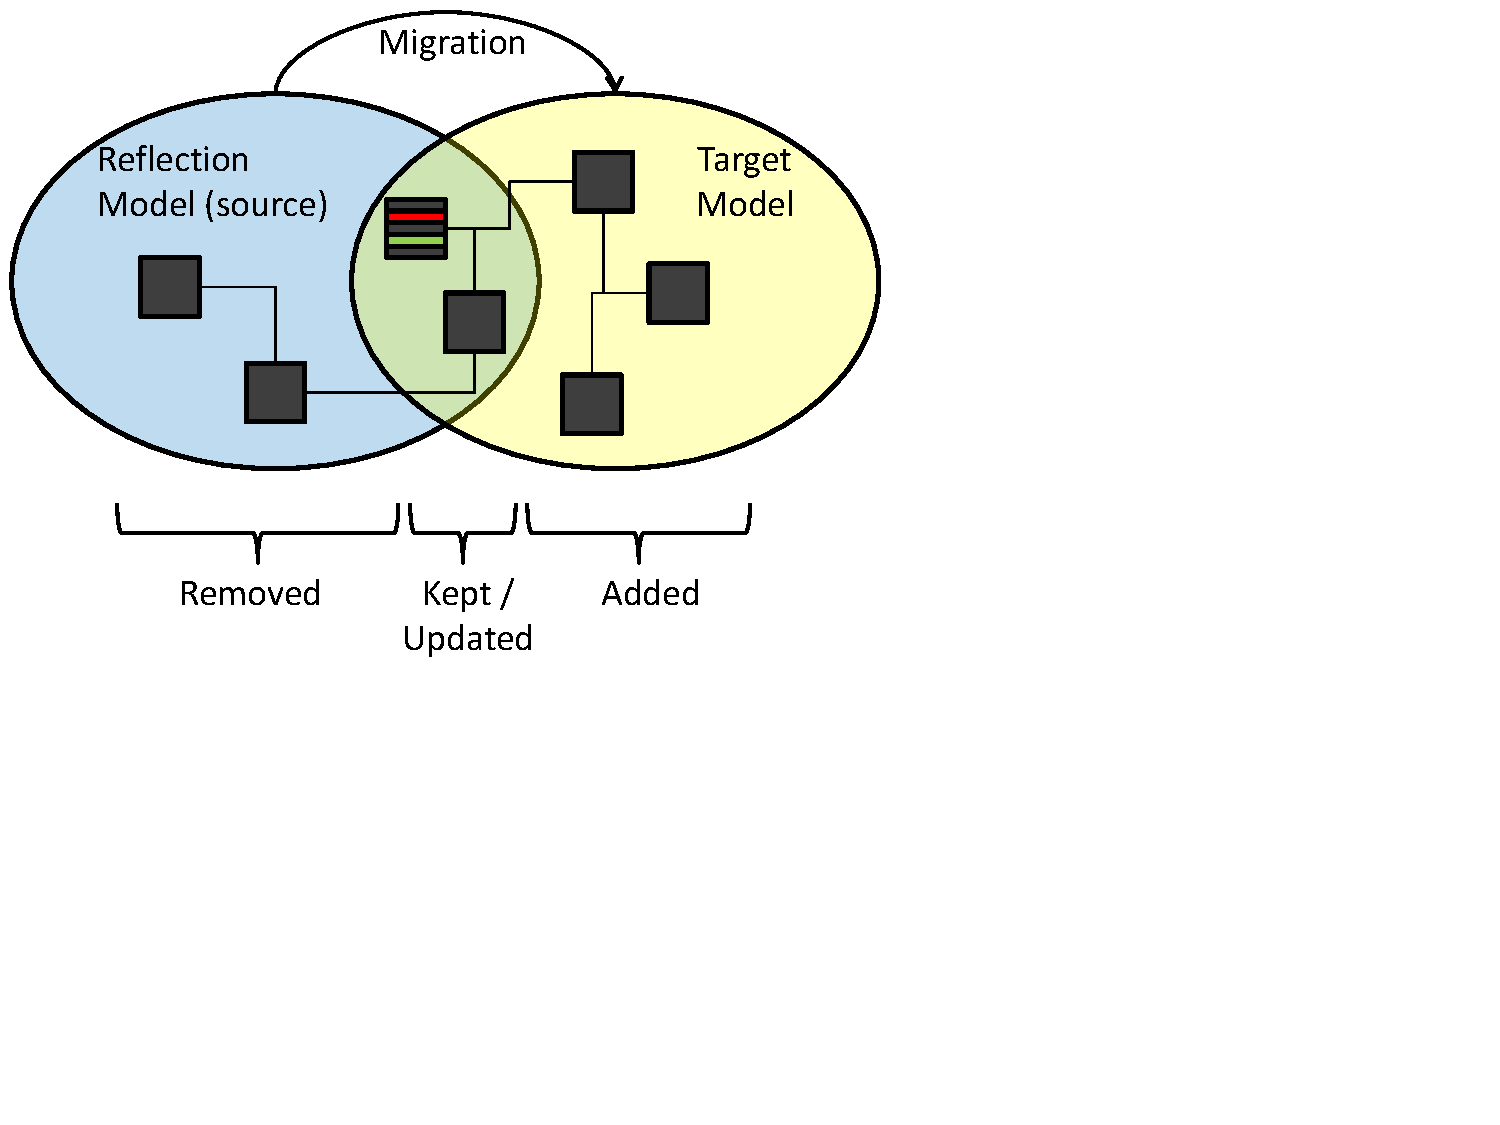
\includegraphics[width=7cm]{part2/pics/comparison}
\caption{\label{figure:comparison} Identifying differences between the source and the target configurations.}
\end{center}
\end{figure}
The steps to go from the current configuration to the required one are specified by primitive commands that represent atomic differences between the two configuration models.
The comparison system only deals with abstract commands, to allow a change of the component management policy. The real commands are instantiated (not yet executed) according to the actual policy, during the model comparison.\\

{\bf Planning the execution sequence}\\
These commands are stored in a collection and ordered according to a heuristic~\cite{Andre:2010} that ensures a safe migration from the current to the target configuration. Before actually executing the commands, the list is parsed to verify that all the commands can be executed. For example, for all {\it AddComponent} commands, the presence of the specific component factory is checked, to ensure all components can actually be added without any problems. Doing this kind of verification for all commands ensures that the command execution will execute properly. If a command is detected as non-executable, a report clearly describes the problem, and no command at all is executed. This way, the system is always kept consistent.\\

{\bf Roll-back abilities}
In case the migration fails, each command is decorated with a roll-back equivalent command. Thus, each command executed before the failure can be cancelled. Moreover, a second protection in place consists in keeping the old model in memory. If everything goes wrong, it is always possible to restart from scratch, and migrate back to the old model.\\

{\bf Specificities of components and services}\\
Because of an adaptation, some links (bindings) between components may appear or disappear, for the system to act differently. In the case of classic components, adding or removing bindings is realized by setting or unsetting a variable. Generally, a component missing one mandatory binding is stopped, because it cannot run any longer. However, in the case of service-based systems such as \enti{}, the component may still offer its services to third-party applications, and thus, should not always be stopped. In other words, a "light component", a virtual representation of a real light, may not be bound to any other component, but might still serve another application for the control of this light.\\
Other behavioral constraints can require more complex actions than just a set or an unset. For instance, if an alarm has been triggered and if the user does not process this alarm, the system must be able to propagate the information somewhere else for the alarm to be treated. The removal of a communication link is structurally correct, but the link may take part in an operation being treated, and so, it has to be kept until the end of the action.\\

As previously explained, real commands for the migration are instantiated according to the current policy of the running system. Real commands can also be specialized for each runtime they have to be applied on. In our context, atomic commands have been instantiated to address a service-oriented runtime. Indeed, this runtime has offered all the facilities required by our approach. This is detailed in section~\ref{sec:soaruntime}.

\newpage
\section{Service-Oriented Runtime Architecture}
\label{sec:soaruntime}

\begin{wrapfigure}{r}{60mm}
  \vspace{-5mm}
  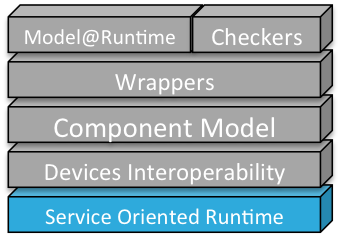
\includegraphics[width=60mm]{part2/pics/layers/SoaRt}
%  \caption{Service Oriented Runtime}
%  \label{fig:soaLayer}
  \vspace{-5mm}
\end{wrapfigure}

For the proposed approach to efficiently cope with dynamic evolutions, the underlying runtime environment is required to offer dynamic abilities. As explained in~\cite{Di-Nitto:2008}, the concept of service has emerged as a good candidate to cope with the dynamicity of adaptive systems. The adoption of this concept led to the development of technologies, standards, and methods to build service-based applications. Since the Service-Oriented paradigm insists on the pervasiveness of services, it naturally imposes service-based applications to properly handle this requirement. Indeed, services can appear and disappear at any time, and applications built upon these principles obviously have to take these constraints into account.\\

The OSGi Alliance~\cite{OSGI:r4}, a 'consortium of technology innovators', has released a set of specifications that define a service-oriented platform, and its common services. This Service-Oriented Runtime has been selected to support commands that require adding or removing component instances and types(binaries), during the execution.\\

{\bf Dynamicity in OSGi}\\
The OSGi kernel is a standard container-provider to build service-oriented software systems. It implements a cooperative model where applications can dynamically discover and use services, provided by other applications running inside the same kernel. It provides a continuous computing environment. Applications can be installed, started, stopped, updated, and uninstalled, without a system restart. It offers a remote management model for applications that can operate unattended or under the control of a platform operator. Finally it embeds an extensive security model, so that applications can run in a shielded environment. According to these specifications, an application is then divided into several bundles. A bundle is a library component in OSGi terms. It packages services that are logically related. It imports and exports Java packages, and offers or requires services. Services are implementations of Java interfaces.\\

{\bf Modularity}\\
Each OSGi bundle is designed to reach the highest level of independence, giving the software enough modularity to allow partial service updates, additions or removals. This programming style allows software-builders to deploy the same pieces of software for all of their clients, either professionals or private individuals and then simply adapt the services installed. Moreover, the services running on the system can be changed during execution.\\

\vspace{0.5cm}
{\bf Component Types, Instances and Bundles}\\
Described in section~\ref{subsec:modelatruntime}, the Model@Runtime engine creates an ordered sequence of commands when it receives a new model to deploy. Each command of the list is then translated into an OSGi command.\\
In \enti{}, component types are contained in OSGi bundles. These bundles are only used as deployment units and do not provide any service. They just embed components. When an {\bf addComponent} command is parsed, the runtime checks if the component type is available in the environment. If not, the bundle containing the type is downloaded and installed. Once the component type is available, a new instance can be created.\\
Component instances are also mapped on bundles because of their independent life-cycle management. Indeed, {\bf start} or {\bf stop component} commands are directly translated to start and stop bundle OSGi commands.\\
\begin{figure}[h!]
\centering
  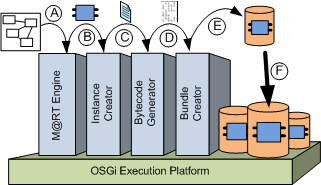
\includegraphics[width=.6\textwidth]{part2/pics/toolchain3.png}
  \caption{Instance creation tool chain}
  \label{fig:instanceToolChain}
%  \vspace{-5mm}
\end{figure}

The creation of an instance is realized as presented on figure~\ref{fig:instanceToolChain}. From the model (step A), a new instance is queried by the Model@Runtime engine(step B) to an instance creator. This instance creator can be a Java code generator, an XML generator, or whatever. The instance creator then asks for the bytecode generator to compile the instance. This compilation can be realized with ASM\footnote{http://asm.ow2.org} for Java code, handled by Spring for an XML file, etc. Step D consists in packaging the bytecode in a bundle. Step E makes it available for the runtime platform. The last step installs the instance bundle in the system.\\

Mapped on OSGi bundles, component instances can offer services to other components in the component model, or to other bundles on the OSGi platform. This facility makes it possible to dynamically expose instances on application-level protocols. This role is supported by the {\it Wrappers} layer described in section~\ref{sec:wrappers}.

\vspace{1cm}
\section{Wrappers}
\label{sec:wrappers}
\begin{wrapfigure}{r}{60mm}
  \vspace{-5mm}
  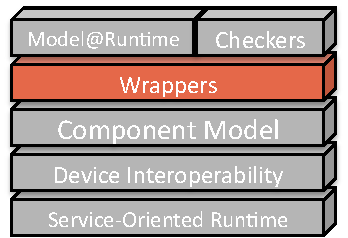
\includegraphics[width=60mm]{part2/pics/layers/Wrappers.pdf}
%  \caption{!!!!!! NO CAPTION !!!!!!}
  %\label{fig:agePyramidEU272009}
  \vspace{-5mm}
\end{wrapfigure}


The wrappers layer takes advantage of the component model layer, which makes it possible to dynamically and automatically wrap devices into several current and future application level protocols. For instance, \gls{upnp}, \gls{dpws} or \gls{dlna} are such kinds of protocols. Their implementations is often too heavy to be implanted into the devices themselves. The role of this layer is thus to export all devices for free, on several protocols. Rather than offering an automatic publication mechanism to a selected protocol, the wrappers layer offers a means to publish any component to any protocol. Each component can thus be accessible using as many protocols as there are wrappers. This approach has been presented in~\cite{Nain08a}.\\

{\bf Component Model {\it versus} Third party}\\
Wrappers need to obtain information about the devices present in a given deployment. This information can be retrieved in two ways.\\
(1) The wrapper is designed as a component. As a consequence, it can monitor the current model of the running system by asking the {\it Model@Runtime} layer. Any change in the model implies that the wrapper check new devices and removed ones. Another benefit of this approach is that a wrapper is considered as a classical component. The model can thus manage it as any other component.\\
(2) The wrapper is built as a third party application, running on the same platform. In this case, the wrapper monitors registrations of services in the OSGi context. Each time a device registers a service, this service is made accessible through the protocol handled by the wrapper. This approach has two drawbacks. Firstly, the export and use of services are not visible in the model. A device can thus be removed while in use through an application protocol. Secondly, the life cycles of the services exported on the application protocol depend on the registration and unregistration of the device's services. Since no dependency is expressed in the model, the life-cycle management of exported services has to be handled 'by hand' by the wrapper.\\

{\bf Reversed drivers}\\
A wrapper is created for each application level protocol. Just as for devices' drivers, the deployment of a wrapper is required for each application protocol to be addressed. Each wrapper monitors the current application to detect addition or removal of devices. For each device, the wrapper takes on the role of a proxy and handles communications to and from the application level protocol.


\section{Summary}
The model used by the Model@Runtime engine has been augmented with the introduction of the component model described in section~\ref{sec:componentModel}.\\
The service-oriented architecture of the runtime makes it possible to cope with evolutions and adaptations, since bundles can be installed and updated with no need to restart the system. These facilities are exploited by the Model@Runtime layer, which comes with tools and methods to address the evolutions, variability, adaptations and safety of the application. However, these properties could not have been used without the creation of a new component model inspired by electronic components. This component model improves flexibility and enables the connection of heterogeneous components, while keeping a high level of reliability thanks to checkers. The Device Interoperability and Wrappers layers provide abstractions of manufacturers' specificities and free publications on application level protocols respectively, to promote interoperability and openness.



\part{Validation}
%\setcounter{chapter}{0}

~\vspace{1cm}
\begin{flushright}
{\it Winners compare their achievements with their goals, while losers compare their achievements with those of other people.}\\
Nido Qubein
\end{flushright}
\vspace{2cm}

\enti{} was tested on a realistic use-case scenario, in which all previously-listed properties were stressed. This scenario, defined in collaboration with partners of an AAL project, is presented this chapter~\ref{ch:aalValidation}.\\

%A second validation has been realized by bringing \enti{} in front of a bundle of end-users, namely elderly people. This study had two goals. The first goal was the improvement of the \gls{gui} widgets presented to end-users, in order to make them as intuitive as possible. The second was the verification that people are able to act on, and get information from the home, according to a pre-define scenario. These two points are detailed in chapter~\ref{ch:itiProject}.\\


\chapter{Validation in the context of an AAL project}
\label{ch:aalValidation}

As one of the IDA project's partners, we proposed \enti{} as a flexible integration tool, for the different types of equipment offered by industrialists. \enti{} has been considered and evaluated on a scenario, collaboratively defined with the partners of the project. It has been designed to underline the properties required for such a system.\\

The first section of this chapter introduces the project and its context and details the scenario used as a validation for \enti{}. Sections~\ref{subsec:interop} to \ref{subsec:opening} describe the evaluation of a set of properties: the environment setup, the procedures, and the results for an evaluated property. Section~\ref{sec:theatsToValidity} lists some threats to the validity of this study. The conclusion and perspectives of these experiments is presented in section~\ref{sec:concluAAL}.

\section{Context of the study: the IDA project}

The first phase of the \gls{ida}~\footnote{http://www.ida-autonomie.fr/} project took place from June 2008 to June 2010, in the City of Rennes and the greater Rennes area(France). This local \gls{aal} project was funded by the Regional Council of Brittany to investigate issues resulting from the ageing of the population, and its socio-economic impact. More precisely, the \gls{ida} project involved conducting an inquiry about the use of \gls{ict} to help elderly people in their everyday life at home. To this end, the project involved:\\
\begin{itemize}
\item[{\bf Association for care at home}] ASSAD du Pays de Rennes
\item[{\bf Industrialists}] Custos, Delta Dore, Urmet Captive, Spartime, i--Pocarte, Domtis, Ordimemo, Intervox Systems, Laudren, Solem
\item[{\bf Social housing authority}] Archipel Habitat
\item[{\bf Installers}] Marsollier Domotique, Lepage Electronique
\item[{\bf Project ownership assistance}] ARELIA
\item[{\bf Research institutes}] INRIA (National Institute of Research in Computer Science and Control), the University of Rennes 1, the University of Rennes 2, LOUSTIC (Information and Communication technology Observation Laboratory), IETR (Rennes Electronics and Telecommunications Institute), CRPCC (Psychology, Cognition and Communication Research Center)
\item[{\bf Public administrations}] Rennes Metropole, Conseil General d'Ille et Vilaine, Ville de Rennes, CCI Rennes, Critt Santé, MEITO
\item[{\bf Elderly people}] Anonymous individuals for tests, obviously
\end{itemize}
The conclusions of the project have been compiled in \cite{ASSAD:2010}.\\

The "ASSAD du Pays de Rennes" Association, leader of this project, employs 450 persons among which, nurses, home care assistants, technicians, etc. The association helps more than 3,000 persons, in 17 towns in the south and east of Rennes.\\

Although the IDA was not funded by the European \gls{aal} program the assisted (elderly) person was project-centred, and the six dimensions described in section~\ref{subsec:aalConcepts} appeared in the background all throughout the project. The ASSAD association took care of this point.\\
\enti{} had been presented as a system for the integration of the several devices evaluated in the project. Indeed, the objective of IDA was to measure how \gls{ict} could foster the autonomy of elderly people at home and support the activity of carers. In this context, we proposed \enti{} as an integration platform, able to deal with various devices and services, and promote the deployment of solutions adapted to each person's needs.\\

Interested in the proposition, collaborative work had been engaged within the IDA project. With the help of the ASSAD, Delta Dore, Custos, Arelia, and the LOUSTIC, among the most active, a scenario was defined to put \enti{} in context.\\
This case study was designed to be as close as possible to real life conditions. The story was introduced by the ASSAD association. Products were proposed by Delta Dore. The evolutions were gathered from past experiences of the ASSAD, Custos and the LOUSTIC. This scenario was set up to evaluate \enti{} on a realistic case, with the same devices as those actually deployed. It stresses several issues to measure how \enti{} would cope with them.\\
The following part of this section presents the story and the evaluation context of \enti{}. The way \enti{} addressed the problems is described for each issue in a separate section.


\section{Use case and issues to address}
\label{sec:usecase}

The scenario used for the evaluation of \enti{} is presented in this section. It involves an elderly person called Mrs P., several members of her family, and different devices selected in collaboration with other partners in order for the evaluation to be realized with real products and in the closest conditions to reality.\\

The scenario is presented here with names of persons and real products for the sake of clarity.\\

The scenario is about Mrs P. She is seventy-eight. She has two children and five grandchildren. Mrs P. begins to experience some difficulties in walking and moving. To improve her safety, her daughter proposed that she moves to an equipped flat.\\
Among other equipment, the flat is basically equipped with an alert system, which triggers a voice call to a care center when a button is pressed on a remote control. But Mrs P. is not comfortable with this equipment and would prefer a more generic remote control. She also would like the alert to be sent to her daughter, instead of to the care center.\\

\begin{figure}[h!]
\centering
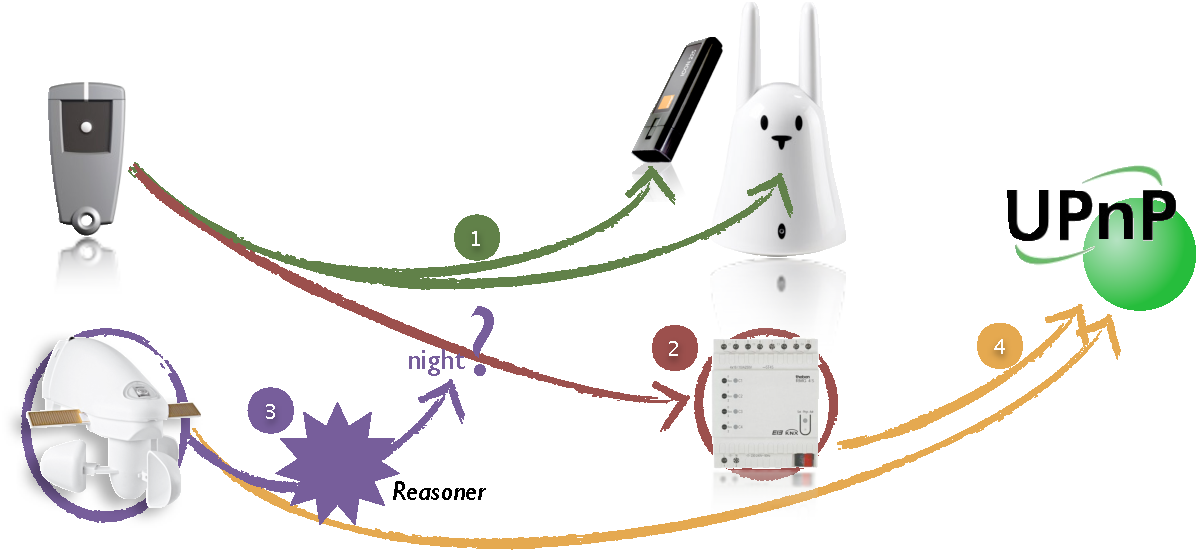
\includegraphics[width=.7\textwidth]{part4/pics/ConcreteApplication}
\caption{Solution elements for Mrs P.}
\label{fig:concreteApplication}
\end{figure}

The remote control, on the top left corner of figure~\ref{fig:concreteApplication}, is a one-button command from Delta Dore (a French manufacturer of home automation devices). This remote control has been designed to be universal for any receiver product from the Delta Dore catalog. A 3G-communication stick (Icon 225) is used to send alerts to Mrs P.'s daughter. Then a Nabaztag rabbit helpfully provides feedback to Mrs P. when she asks for help from her daughter.\\
The connection of these three items raises {\bf interoperability} problems (symbolized by the bullet number one), which are detailed and answered in section~\ref{subsec:interop}.\\

After some months of use, Mrs P. asks for the system to automatically switch on the lights, when an alert is sent. Luckily, the flat is already equipped with devices that enable the control of lights. The light control is made available by a \textit{RMG4S} device from Theben (on the bottom right of figure~\ref{fig:concreteApplication}, working on a KNX network. Section~\ref{subsec:evolution} presents how \enti{} enabled this {\bf evolution}.\\

Following this evolution, the behavior of the lights was sub-optimal, because the lights were switched on whatever the period of the day. To eliminate this issue, an {\bf adaptation} mechanism(bullet 3), described in section~\ref{subsec:adaptation}, was deployed. The sensing of daylight was realized by a KNX weather station outside the house. This weather station is visible on the bottom left corner of figure~\ref{fig:concreteApplication}.\\

One day, her son came with a new device. This touch screen would allow Mrs P. to easily access the Internet and to have video calls with her children and grandchildren. The touch screen also has abilities for controlling devices over \gls{upnp} and \gls{dpws} networks. Since then, the deployed solution is required to be compatible and therefore it is required to export all available devices on \gls{upnp} and \gls{dpws}. This requirement stresses the need for {\bf openness}. Section~\ref{subsec:opening} elaborates about the mechanisms used to answer the fourth bullet of figure~\ref{fig:concreteApplication}.\\


In order to evaluate the answers of \enti{} in this scenario, and since a real deployment cannot be realized, a test environment with real devices was set up. Just before the description of the solutions offered by \enti{}, the different elements composing this environment are presented in section~\ref{sect:envDeTest}.


\section{Experimental setup}
\label{sect:envDeTest}
The test environment of this study was realized with equipment provided by industrial partners of the IDA project for one part, and funded by the HID platform, financed by a European Regional Developments Fund for the other part. It is mainly composed of two home mock-ups, one with Delta Dore devices exclusively, the other with KNX devices exclusively and an MSI Top touch-screen PC, as visible in figure~\ref{fig:equimentsForTheStudy}.

\begin{figure}[h!]
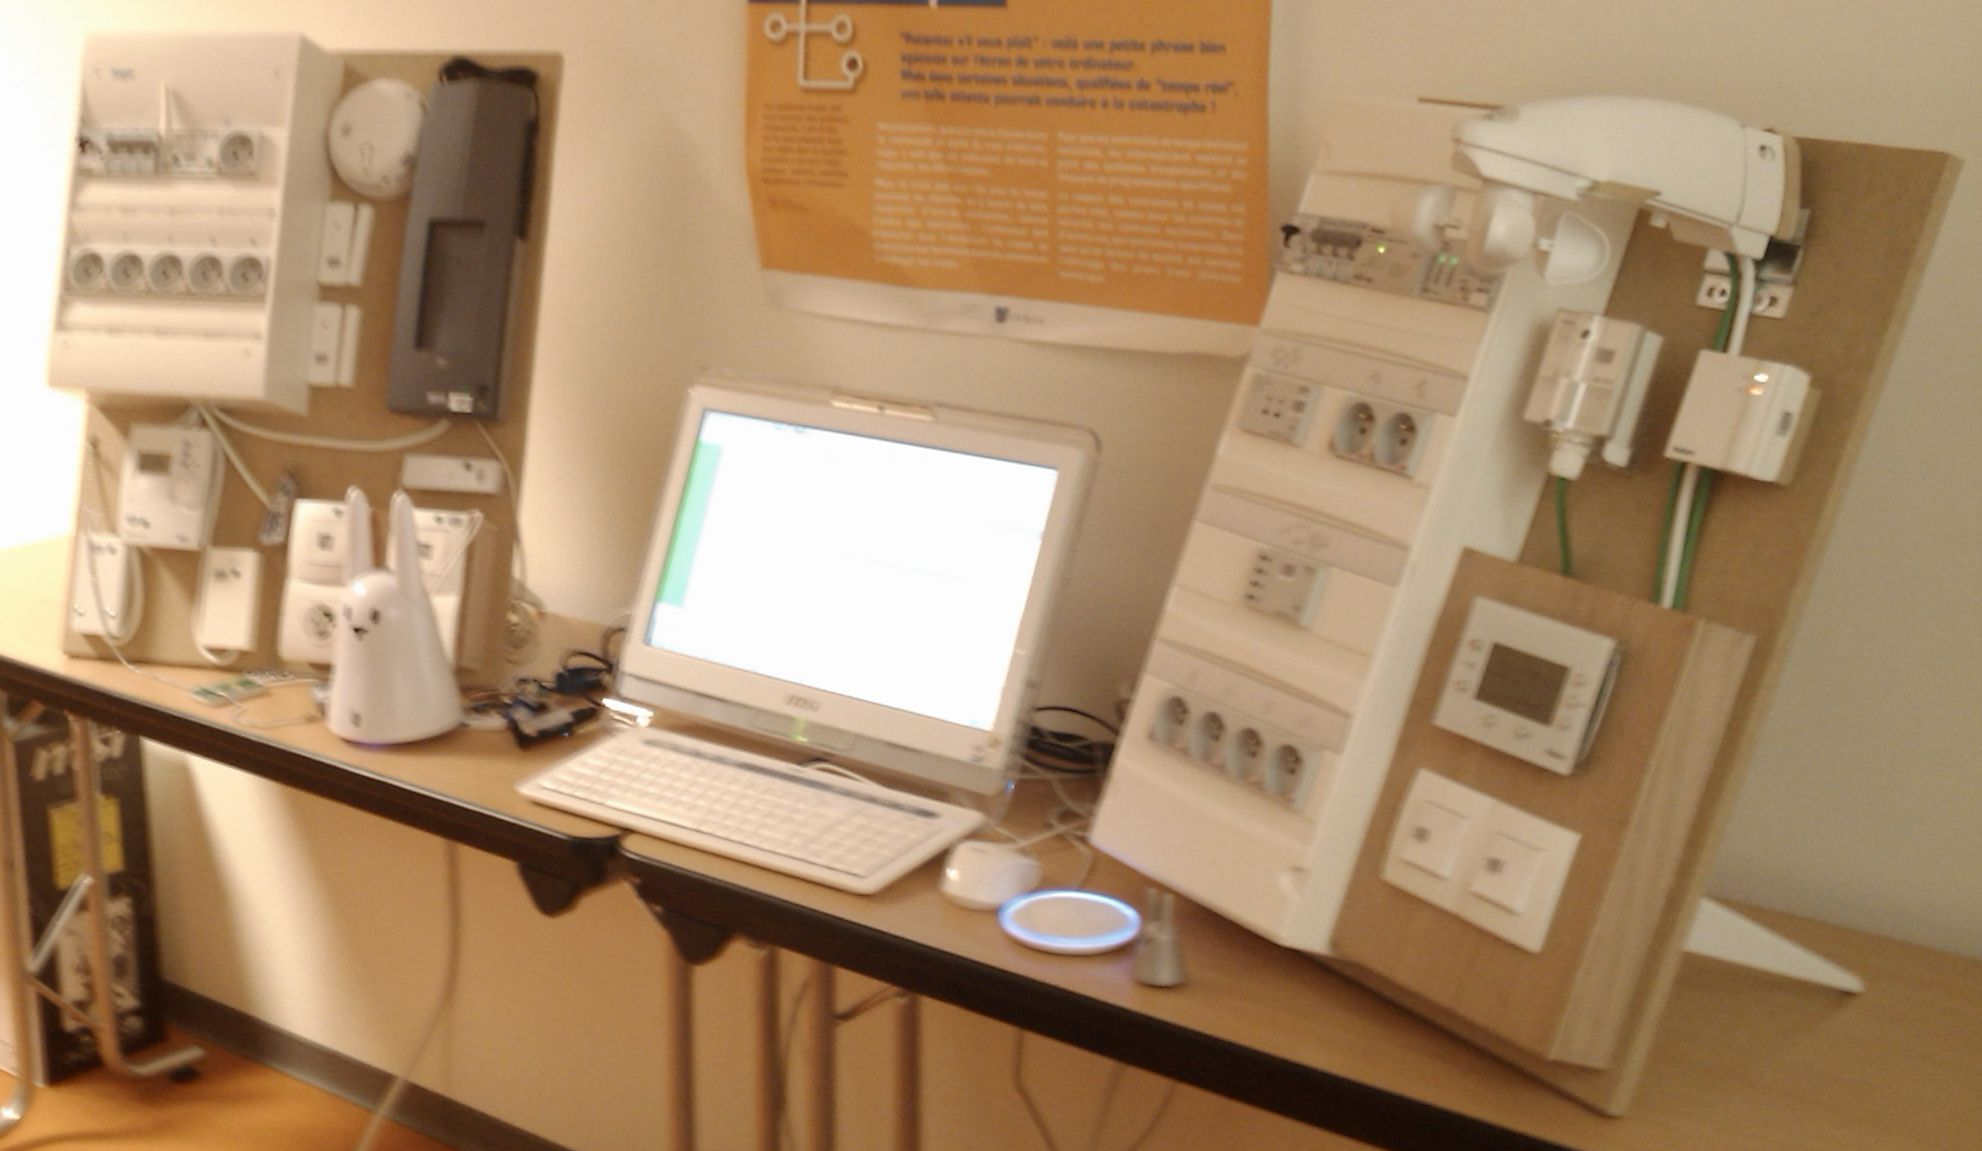
\includegraphics[width=\textwidth]{part4/pics/maquettes.jpg}
\caption{Equipments available for the study}
\label{fig:equimentsForTheStudy}
\end{figure}

\subsection{Delta Dore equipment}

The Delta Dore mock-up, visible on the left side of picture~\ref{fig:equimentsForTheStudy}, was set up with devices from heating, alarm, security and automatism functional domains. Here is the description of all the elements.\\
\begin{itemize}
\item A {\it DRIVER 210 CPL + TYDOM 520} heating controller, on the bottom left corner of the mock-up, controls two heater receivers: a {\it TC51089} \gls{plc} receiver, and a {\it RF660FP} radio receiver.
\item The big black box on the top right corner of the mock-up is a {\it TYXAL CSX40} alarm, which collects information from several sensors. A {\it DOFX} smoke sensor, and two {\it MiniCOX} door sensors, visible on the left side of the alarm. The last sensor is a {\it DFX} water leak sensor (green object on the table, under the mock-up).
\item One {\it TYXIA 442} light dimming transceiver, and a {\it TYXIA 411} timed power switch, both hidden behind the rabbit.
\item Not visible in the picture, two remote controls. One {\it TYXIA 110} with a single ON/OFF button, and a {\it TYXIA 141} with four.\\

\end{itemize}

All these elements use the X2D protocol, owned by of Delta Dore, to communicate on both PLC and radio media. Since the protocol is not public, Delta Dore lent us a research and development product, able to communicate in both ways (listen and act) on the X2D network.\\

\subsection{KNX equipment}

The second mock-up, on the right side of the picture, is made of KNX compatible products only, mainly from the manufacturer Theben and some from Siemens.\\

\begin{itemize}
\item On the top right corner of the KNX mock-up is an outdoor weather station. This weather station gives information about the wind, the rain, the temperature, and the light value. This information can be provided whether periodically or when a value changes slightly.
\item Just under the weather station, on the left, the {\it LUNA 113} is a light sensor for the outside. On its right, an {\it AMUN 7160} provides information about temperature, humidity and $CO_2$ rates inside the house.
\item Going down the right side comes the {\it VARIA 826 WH KNX}, which is an ambient controller. It allows for changes in the heating regulation values, reading information from the weather station and many other appliances.
\item The four switches, in the bottom right corner of the mock-up, are controlled by a {\it TA 4}.
\item The electric panel includes three other devices. An {\it RMG4s} device controls the four power sockets, at the very bottom of the panel, with a On/Off behavior only. Above this device, a {DMG 2} controls the dimming of the two sockets on its right.
\item Hardly visible on the top of the panel, a Siemens {\it EIB/IP N148/21} gateway makes it possible to access the KNX network through an IP connection. Helped by the Calimero~\footnote{http://calimero.sourceforge.net} framework, it enables a programmatic control on all the devices, and allows the user to listen for events on the KNX network.
\end{itemize}

\subsection{Other equipment}

The link between all of these devices is made by \enti{}, but it still requires an environment for its execution. Several other devices are available in this experimental setup.

\begin{itemize}
\item An all-in-one PC {\it MSI Wind Top}, with a touch screen, an Intel Atom 230@1.6GHz CPU, 1Gb RAM and Ubuntu 9.10 (Linux kernel: 2.6.31-17-generic) for the operating system. 
\item An {\it Icon 225} 3G USB modem, used only for sending short text messages
\item A Nabaztag:tag, the big rabbit in the picture, able to synthesize a voice from a text, and used to provide feedback to the user. A Nanoztag with a Mir:ror (little grey rabbit and round blue base) are used as an \gls{rfid} tag and an RFID reader respectively.
\item An Ethernet router to connect the KNX mock-up and the touch-screen.
\end{itemize}



\section{Interoperability issue}
\label{subsec:interop}

The first problem that the story of Mrs. P emphasises, is the connection of three heterogenous devices.

\subsection{Test Environment}
To evaluate \enti{} on this issue, we made use of the Tyxia 110 remote control from the Delta Dore mock-up, the 3G modem to send text messages and the Nabaztag:tag rabbit to provide feedback to the end user.\\
Nothing in \enti{} was already available to access these products.\\
The MSI Top touch-screen was used for the deployment of the test.

\subsection{Resolution Protocol}

{\bf Driver creation}\\
Each product used in this test is from a different manufacturer. Thus, three drivers had to be created, as described in section~\ref{subsec:useOfDrivers} of the contribution.\\

The driver enabling the use of the Tyxia 110 makes use of the gateway offered by the manufacturer, making it possible to listen on the X2D network. This gateway was delivered with a Java API, which simplified the creation of the driver. Indeed, the driver just consists of the creation of a listener and of a class to handle the implementation and the model of the remote control device. The Tyxia 110 component has a unique output port {\it pressed}, and can be customized to specify the parameters to be sent through the output port when the button is pressed.\\

The second element, the 3G modem was considered as a simple modem. The sequence of {\it AT} commands to be sent to the modem, to send a short text message, was collected from the modem documentation. With the help of a serial communication library in Java (RxTx), the component was implemented, and decorated with modeling annotations. The Icon 225 component representative offers a unique input port {\it send}. This port admits one parameter: the text of the message to send. The receiver's phone number is given as a parameter to the component.\\

The Nabaztag:tag rabbit is the last element in this test and is used to provide feedback to the final user. The web-service API of the Nabaztag rabbit provides a Text-To-Speech facility that can generate and return an MP3 file. Indeed, the rabbit is able to either, directly synthesize a voice from a text or generate a file containing the voice synthesis, for it to be played later by the rabbit. The component standing in for the rabbit thus proposes a {\it generate} input port. The action of this port is to call the text-to-speech facility with the text passed through the port as a parameter. The generated MP3 file is then returned through an output port called {\it generated}. A second input port, {\it play}, can be used to ask the rabbit to read a text or an MP3. If a text is given in parameter, the synthesis is made on the fly.\\

\begin{figure}[h!]
\centering
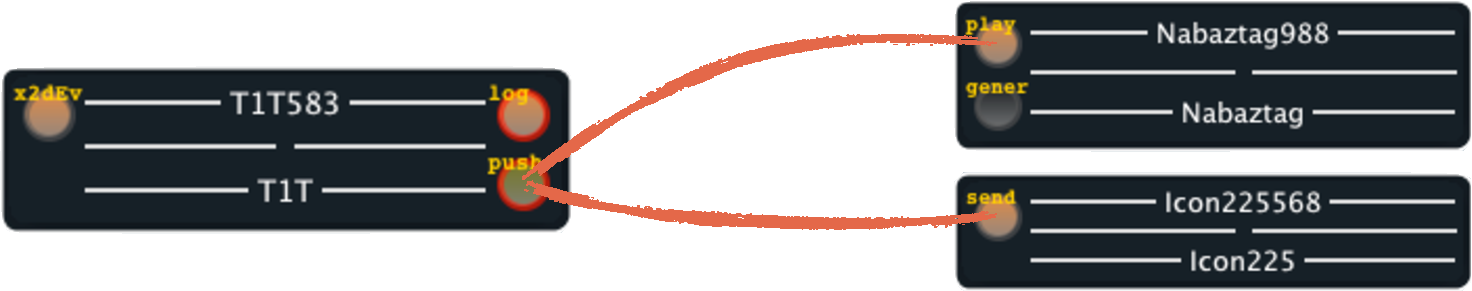
\includegraphics[width=.7\textwidth]{part4/pics/validInterop}
\caption{Components used in the interoperability experiment}
\end{figure}

{\bf Connection of the elements}\\

An instance of each element of the assembly is created in the model. The Tyxia 110 is customized to send two parameters through its output port on activation: the text "Your request has been sent to your daughter." for the rabbit, and "Your mother is requesting a call from you." for the Icon 225.\\
This message with the two parameters is forwarded to a dispatcher, which triggers in parallel the {\it send} input port of the Icon 225 instance, and the {\it play} input port of the Nabaztag. Each component collects the parameter it is interested in and carries out the required action.\\

\subsection{Results}

At first sight, the connection of a generic remote control, an electronic rabbit, and a short message modem is not that obvious. Industrial partners of the project were baffled by this requirement, because it implied that they develop an ad-hoc device. This is not viable when targeting a provision of specialized solutions for each person's needs.\\
%\enti{} makes this problem quite easy to solve.\\

In this example, three drivers had to be developed to be able to get components in the model. Each driver can now be augmented to provide more products from each manufacturer. The development of drivers, once done, is never to be done again. Components can also be reused in other contexts, because of their independence and the avoidance of direct connections. For future applications, this signifies a great gain in time.


\section{Evolution issue}
\label{subsec:evolution}

The evolution in this use case is due to a change in Mrs P.'s needs. She wants the lights to be automatically switched on when she presses the remote control. This requirement is related to a feeling of safety when lights are on at night.\\

\subsection{Test Environment}

This evaluation makes use of the previous devices involved in the interoperability evaluation.\\
In addition, the RMG4s of the KNX mock-up are integrated in the application.

\subsection{Resolution Protocol}


No KNX product had been used for the moment. So, the first task was to create the driver to control KNX equipment and obtain a model representative for the RMG4s (presented in figure~\ref{fig:rmg4s} a few pages back). Once the component is ready, it has to be deployed.\\
Thanks to the Model@Runtime layer, the technician responsible for the addition of the new functionality retrieves the current model of the running application, using a TCP/IP remote access. He then adds an instance of RMG4s and connects all {\it on} input ports to the dispatcher already present. In this configuration, all lights controlled by the RMG4s are lit when the Tyxia 110 button is pressed, in addition to the text being sent and the rabbit speaking.\\

\begin{figure}[h!]
\centering
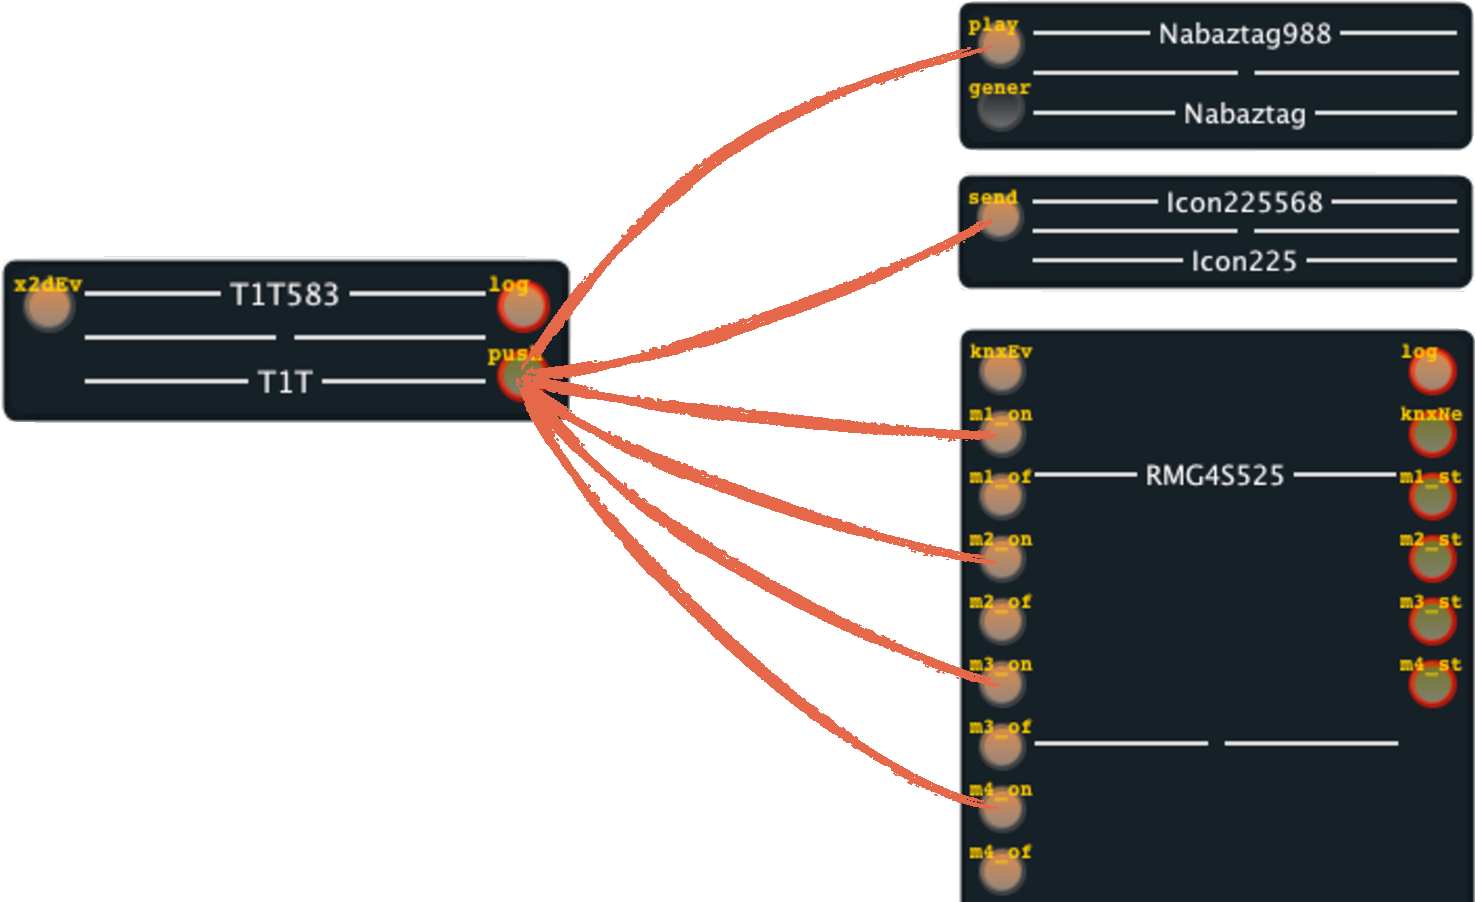
\includegraphics[width=\textwidth]{part4/pics/validEvol}
\caption{Components used in the evolution experiment}
\label{fig:validEvol}
\end{figure}

For the last step, the technician sends back the model to the runtime of \enti{} in the home. Once all checks are passed, the runtime downloads the newly-created component type and its driver, in order to create and connect the instance. All this procedure is transparent for Mrs P., who is called just before and after the operation to keep her informed. The OSGi runtime prevents any service interruption.

\subsection{Results}

Again, a driver had to be created as well as a component to handle the RMG4s. Thanks to the Model@Runtime engine, the technician was able to collect the model and modify it. He then asked the runtime for the deployment of the new model. Realized through a TCP/IP connection, this evolution could have been realized remotely. This ability reduces the disturbance for the helped person, and can reduce the time from the query to the realization.\\
For this experiment, the communication with the runtime used a TCP/IP connection, which may not be that easy in real life.


\section{Adaptation issue}
\label{subsec:adaptation}

The behavior of the lights was sub-optimal after the deployment of the evolution. Indeed, the lights were switched on, whatever the period of the day, every time the remote control was pushed. To remedy this issue, an adaptation mechanism (presented in \cite{Nain10a}) was deployed. This mechanism changes the configuration of the system, according to the external lighting value sensed by a KNX outdoor weather station.

\subsection{Test Environment}

In addition to the previous equipment, selected for interoperability experiments and evolution concerns, the outdoor KNX weather station is now included in the configuration.

\subsection{Resolution Protocol}

The driver for KNX products already exists. The unique thing to implement is a component representative for the weather station.\\

The Model@Runtime engine offers means to connect reasoners. A reasoner is able to modify (or ask for the modification of) the running system configuration. The decision is made locally according to some contextual information. This information can be as simple as a value change, or as complex as an aggregation of events.
For this evaluation, a reasoner has been created to modify the connections of the {\it RMG4S} according to the period of the day.\\

The system is currently composed of five components. A {\it TYXIA\_110} remote control, a dispatcher connected to a 3G USB stick to send texts, and to a Nabaztag rabbit to inform Mrs P. In addition, the RMG4S makes it possible to control the lights. {\bf At night}, this configuration is the one required. {\bf During the day}, the RMG4S should not be activated, and the connections with the dispatcher have to be removed.\\

\begin{figure}[h!]
\centering
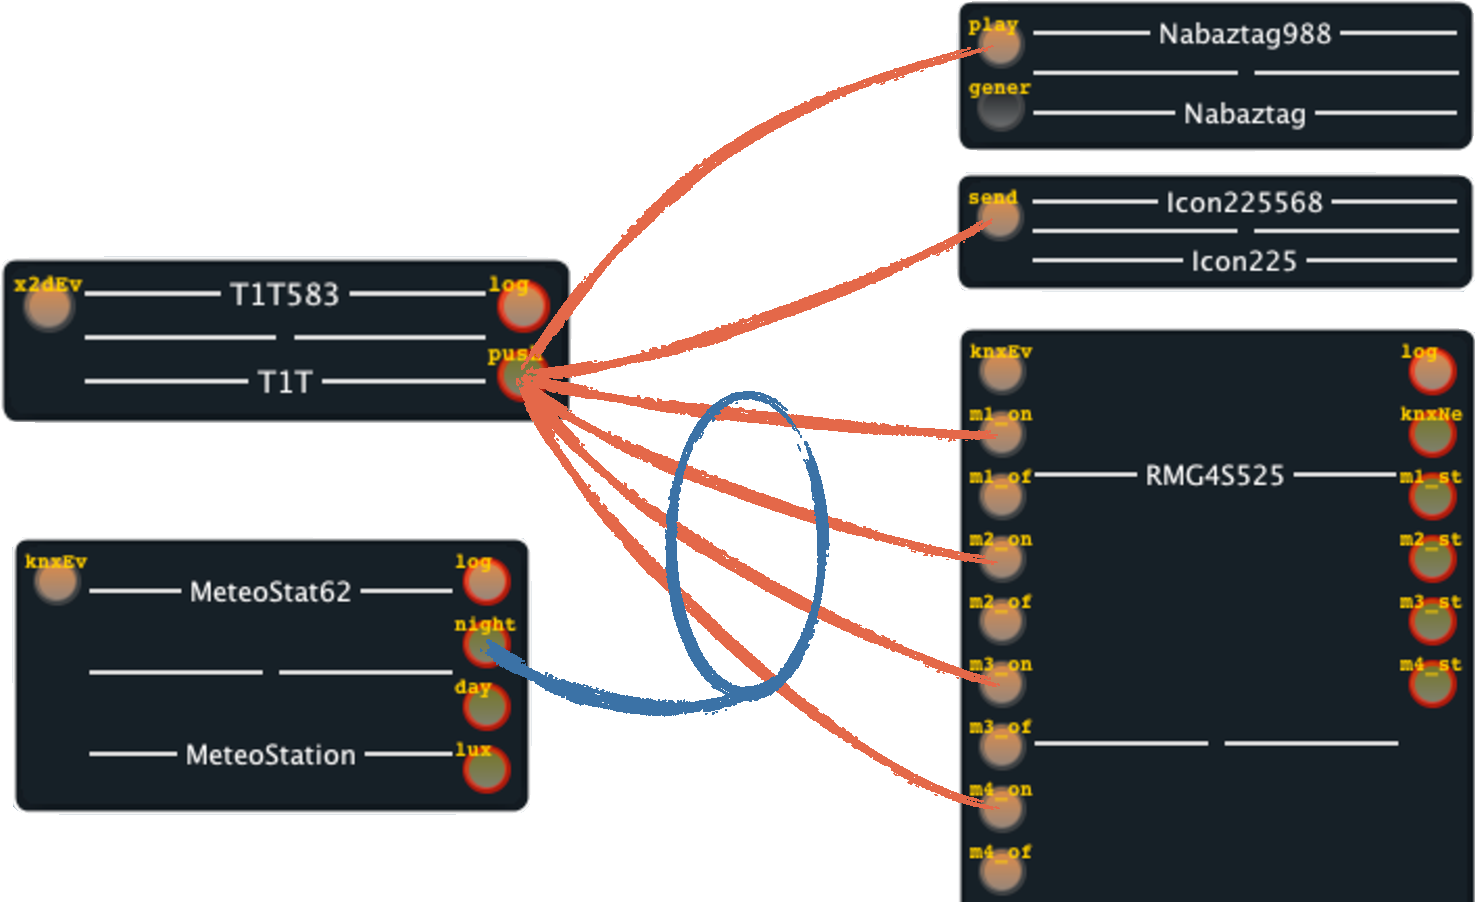
\includegraphics[width=\textwidth]{part4/pics/validAdapt}
\caption{Components used in the adaptation experiment}
\end{figure}


The weather station has been added to the system as described in section~\ref{subsec:evolution}.\\

To be able to perform execution time bench testing, the experiment including the reasoner was deployed from scratch.
The MSI Top was cleaned of any previous binary element and restarted. The deployment was then realized as follows:\\

{\bf Initial Deployment} The initial deployment is realized during the day. The model deploys only the remote control, the rabbit, the USB stick, the dispatcher, and the weather station. In this configuration, the elderly person can ask for help by pressing the Tyxia 110 button, just as before, but no light is switched on.\\
 
{\bf At night} The reasoner adapts the system to the new conditions. It changes the model by adding an RMG4S instance and all necessary connections to the dispatcher.\\
 
{\bf Day} When the day returns, the reasoner removes the connections and the instance of RMG4S.\\

\subsection{Results}

Figure~\ref{figure:bench} presents the execution times measured while a sequence of reconfigurations of the system was run. This sequence consisted of five steps. After the initial deployment (\textit{State 1}), the scenario iterates night states (\textit{State 2} and \textit{State 4}) and day states (\textit{State 3} and \textit{State 5}) during the next two days.\\

\begin{figure}[h!]
\centering
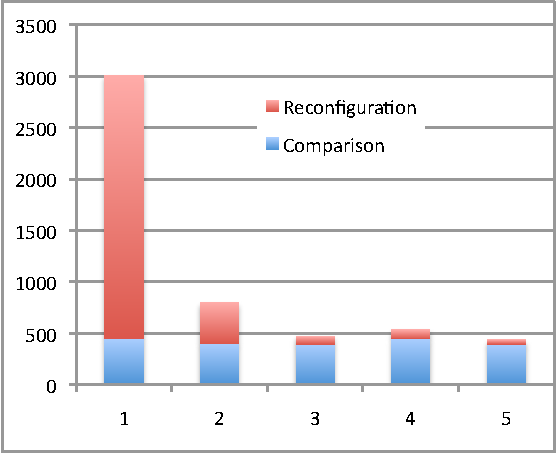
\includegraphics[width=7cm]{part2/pics/benchs_graphic3}
\caption{ Time (in ms) spent in Configuration Comparison and Actual Reconfiguration}
\label{figure:bench}

\end{figure}

As the  worst case scenario has been considered, the system is initially empty. Starting from scratch, all components need to be deployed during the initial configuration. In particular, all the component types have to be downloaded and checks have to be performed on the entire model. It explains the rather long reconfiguration time of step 1:  2.5 seconds. \\

The first reconfiguration (day $\rightarrow$ night, step 2) implied the deployment of an instance of RMG4S and the creation of bindings. As this component has never been used before, its component type is not present and has to be downloaded. All other components already deployed are reused. The downloading and deployment of the component type, plus the instance creation and its bindings to the dispatcher, are realized in less than 400 ms.\\

The next 3 reconfigurations (night $\rightarrow$ day $\rightarrow$ night) are much faster. Step 3 simply consists in unbinding and removing the RMG4S component. Step 4 is similar to step 2. Component types are not uninstalled. The RMG4S component type is thus immediately available for an instance creation. Step 5 is similar to step 4. The actual reconfiguration time of these steps is less than 100 ms.\\

For each reconfiguration, a model comparison is performed by the Model@Runtime engine, prior to the real deployment. This comparison detects changes and creates the commands' sequence for the transition. This model comparison takes an almost constant time of 400 ms. Executed before the actual reconfiguration, the comparison delays the reconfiguration of the system, but does not impact the duration of dynamic reconfiguration. \\



\section{Openness issue}
\label{subsec:opening}

As presented in section~\ref{sec:usecase}, the system was required to expose the devices on both \gls{upnp} and \gls{dpws} networks. The next two sections describe how components have been automatically wrapped to be available on these networks. They report an actualized version of the work presented in~\cite{Nain08a}.


\subsection{UPnP export}

UPnP~\cite{UPNP} is based on a discovery-search mechanism. As a UPnP-Device joins the UPnP network, it sends an XML description file to all UPnP-ControlPoints. This file presents the device with information such as manufacturer, device type, device model, or its UUID. Most of times a UPnP-Device is self-contained.\\
It is able to describe itself and the services it publishes on the network. The description structure, visible on the upper part of figure~\ref{fig:upnp-mapping}, is organized as follows.\\
UPnP specifications allow devices to contain other devices (called embedded devices). In this case, the container (called the {\it rootDevice}) takes the responsibility for publishing information about itself and each device it embeds.\\
Each service a device can offer has to be described in a separated file. This file characterizes all the UPnP-Actions the service renders, and all the UPnP-State Variables used by these actions. UPnP-Actions can admit parameters. These parameters have a direction (in or out), a name, and a related StateVar. UPnP-StateVars handle information such as value types, or lists of allowed values for a parameter.\\


\subsubsection{Test Environment}

This experiment required some devices to be deployed on the runtime for them to be exported. We chose to fix the system in the night state of the previous experiment, thus with a maximum of devices present in the system.\\
This test also required a third party tool to act as a UPnP external control point. This was the touch screen provided by Mrs P.'s son. Since \enti{} was deployed on the MSI Top, we made use of a toolkit from Intel: "Intel® Tools for UPnP Technologies (Build 2777)". This toolkit is no longer maintained and is only available for Windows.

\subsubsection{Resolution Protocol}

{\bf Mapping UPnP devices to \enti{} devices}\\
Although \enti{} devices and UPnP devices are quite similar, they are not exactly aligned in their structures. However, the mapping (blue arrows in figure~\ref{fig:upnp-mapping}) was quite natural. \enti{} devices were mapped on UPnP devices.\\
\enti{} devices can provide two kinds of ports: service and messages ports. {\it NB: only input ports are considered here}. Services ports are composed of operations. This kind of ports was associated with its UPnP equivalent, namely Service for the port, and Action for the operations. The closest UPnP element to handle message ports from \enti{} is the concept of {\it Actions}. Indeed, a message port provides only one service/action. As a consequence, there are as many services as there are message ports created. Each service proposes a single action, which connects to the message port.\\

\begin{figure}
\centering
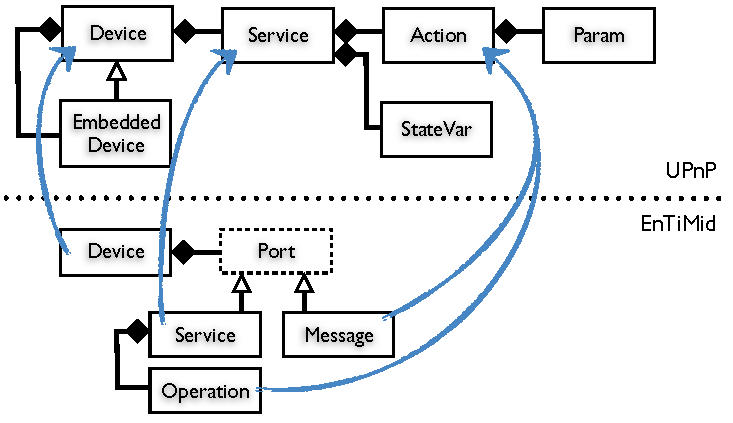
\includegraphics[]{part4/pics/UPnPMapping}
\caption{Mapping UPnP-EnTiMid}
\label{fig:upnp-mapping}
\end{figure}

{\bf Generation of description files}\\
In \enti{}, each component is described by a model. The model is a graph of objects at runtime and is serialized in an XML file. The generation of the XML description file for UPnP is thus quite natural.\\
The service descriptions are the first files to be generated. For each \enti{} service, a new file is created. Operations of the service are then described in the UPnP formalism. Not all operations are described, due to a sometimes complex translation between \enti{} and UPnP runtimes. In any case, all simple methods are included in the description. In the same way, a new service file is created for each message port. The service takes the name of "<port>on<component>" for the services to be differentiated. Each service of this kind is composed of a unique action whose name is identical to the one of the port.\\
Afterwards, a separate description file is created for each component available on the system. The description of a device in UPnP is threefold. The first part provides general information about the product such as the name of the manufacturer, a brief description, the model type, the model number, or its serial id. If not available in the model, these elements are automatically generated, or completed with default values. The second part contains the list of the services a device provides. This description makes reference to the service description files previously generated. The last part contains information about the embedded devices. For each of them, the two previous parts have to be specified.\\

When a UPnP-ControlPoint starts, it broadcasts a query for descriptions of devices available on the network. The UPnP wrapper then sends the description files of all devices and services provided in response.\\

{\bf Runtime elements}\\
The generation of description files is necessary, but not sufficient for UPnP queries to be forwarded to the real device. Indeed, no connection was made between the real runtime component standing for the devices and the UPnP network. To cope with this issue, virtual abstract \enti{} components are created at runtime. Each real device exported on the UPnP network is linked to an abstract component responsible for the handling of communications between the real device and the network requests. These abstract components only have output ports. {\it i.e.}: an output port is specially created on the abstract device to be connected to each input port of the real device exported on the UPnP network.\\
Then, queries are routed by the UPnP exporter to the abstract component in charge of the concerned device. The abstract component activates the input port of the real device according to the request.\\

\subsubsection{Results}

Once the wrapper is deployed on the MSI Top, the Nabaztag rabbit, the 3G USB stick and the RMG4S were all made available through the UPnP network. Indeed, we were able to view and act on these devices from a remote PC equipped with Windows, and the Intel UPnP toolkit.\\
The low number of tools that accept the discovery of self-describing UPnP devices can be a limitation for the use of this wrapper.


\subsection{DPWS export}


\gls{dpws}~\cite{DPWS} defines a minimal set of implementation constraints, to enable secure Web Service messaging, discovery, description and eventing on resource-constrained devices. Its objectives are similar to those of \gls{upnp}. The difference is that DPWS is fully aligned with Web Services technology and is designed to work upon a web-service transportation protocol. It also includes numerous extension points, to allow for seamless integration of device-provided services in enterprise-wide application scenarios.\\
From a conceptual point of view, the DPWS structure is close to that of UPnP, described in figure~\ref{fig:upnp-mapping}. Consequently, the mechanisms to map \enti{} devices and their \gls{dpws} representative follow the same idea. Nevertheless, the generation process is different. Publications to the DPWS network have been realized thanks to the WS4D project~\cite{ws4d}. In their approach, each DPWS-compatible device has to extend an abstract DPWS device, proposed by the framework they provide. The reason is that this abstract component handles all web service-specific communication concerns. The creation of a virtual component is not sufficient in this case. A source code has to be generated.\\

\subsubsection{Test Environment}

Since UPnP and DPWS are very close in terms of needs for devices to be exported, the same set of devices was selected for this experiment.\\
As for UPnP, we made use of an external tool to check that the export of devices was made properly. The experiment was carried out using a second PC equipped with a DPWS explorer\footnote{http://ws4d.e-technik.uni-rostock.de/dpws-explorer/} to list and act on published devices.

\subsubsection{Resolution Protocol}

{\bf DPWS devices creation}\\
For each device, service and operation, a Java class has to be generated. According to the element they represent, classes must extend {\it HostedService} for services, {\it HostingService} for devices and {\it Action} for operations. Parameters are instances of the class \textsf{Parameter}. Luckily, all these classes still can be generated with an automated process. To achieve the code creation, the JET Framework has been used. Templates of DPWS files were set up and they are used at runtime to produce Java classes.\\
More than just Java classes, the generated files are also implementations of new component types. These types are the wrappers of real devices for DPWS. These components are thus responsible for the direct connection between model elements and DPWS controllers.

{\bf Compilation and use}\\
The generation process produces Java classes, but no binary code. These classes still have to be compiled to be useful at runtime. The decision was made to embed the JDT compiler provided by Eclipse. As a result, the bundle to export devices through DPWS is a bit heavy. The compilation is also resource-consuming for quite a small computer device. Once compiled, these classes are packaged into a bundle, which is then deployed on the OSGi runtime.\\
Classes are then handled just as classical components. The tool asks for new components to be added in the runtime, and they are bound to the device  they export.\\

\subsubsection{Results}

Obviously, this is not optimal but it works, since we were able to see all devices and act on them using the DPWS Explorer tool. Other solutions involving more powerful servers in charge of the transformation from a model representation to a component type bundle have been proposed, but not yet completely realized. In any case, the principle is just to extract a tool chain that already works.\\


\section{Threats to validity}
\label{sec:theatsToValidity}

\subsection{Internal threats}

\subsubsection{Variability management}

Variability management, described as being an important issue in home automation for assisted living is not addressed in this experiment.
Indeed, the scenario considers a unique deployment, for a single person, in a single home. A second round of definitions of a more global scenario may have stressed this requirement for variability management.\\
Nevertheless, a lot of work has been carried out to try to cope with this issue, such as an approach using Aspect-Oriented Modeling presented in \cite{Morin09a}. Other perspectives to address this question are presented in section~\ref{sec:archiSynth}.

\subsubsection{Scalability}

The scenario did not highlight any issues about the distribution or scalability of the solution for deployment on a town-wide or even a countrywide scale. 
This scalability validation will be addressed in the future with real deployments.\\
The MSI Wind Top, on which the experiments have been led, may not be the unique platform on which to test \enti{} and a large-scale vision scenario would have highlighted this.\\

\subsubsection{Safety and Security}

Voluntarily, we decided to distance ourselves from access security and privacy considerations. Not because they are not essential, but because they impose such heavy constraints that the search for a technical solution may have been compromised. Now that the system is clearly designed and that the proof of concept has been validated, work to secure communications and data has to be realized prior to any real deployment.\\

Concerning safety, our experimentations did not require complex checks on models. Only simple structural checks, to find cycles for instance, were implemented and used.
In our approach, type checkers and validation policies have been designed to be customized according to the application domain and its constraints. Thus, their complete definition would have been useless in the context of the experiment. In the case of real deployments, they have to be completed to verify that no configuration identified as a case of failure is asked for deployment.

\subsection{External threats}

\subsubsection{Validity of the scenario, real deployment}

The experimentation scenario, even when defined in collaboration with several players in the AAL domain may not consider all cases. The interface between people coming from a technical field and people coming from social field is quite difficult to find. Because people in social activities are not aware of what it is possible to do with technologies and because industrialists are not aware of the everyday problems the dependency of persons can raise, the discussions can rapidly come to a dead end.\\
The scenario validated for this study was accepted by all sides, but may be limited by the comprehension each side had of the problem.\\

\enti{} has been instantiated and validated on a virtual case. A real deployment would have highlighted other issues, other constraints not addressed in this evaluation. This real deployment is part of the perspectives for this work.


\subsubsection{Communications with smart devices}

Gateways are essential for us to be able to communicate with smart devices. For instance, the bi-directional communication with Delta Dore devices was made possible by an R\&D product. Otherwise, the {\it TYDOM 350}, an embedded web server, is the only device they commercialize to act on their devices. This one only enables users to act on devices through a web page interface. This product does not detect any event on the X2D network; it just acts on devices (with no acknowledgement by the way).\\
\enti{} is not able to use any device without a means of communication with it.

 

\section{Conclusion}
\label{sec:concluAAL}

An experimentation using real devices was set up by a collaborative work of the project's partners to evaluate \enti{} on a scenario as realistic as possible. Made with the background of each partner, this scenario was designed to stress several issues identified on this kind of integration systems.\\
\enti{} passed the main requirements highlighted by the scenario and required for such systems to be deployed. This validation comfort the idea of making \enti{} an integration platforms to offer customized solutions for each person's needs.\\
Some limitations due to the lack of real and large scale deployment have been identified. These limitations will probably be addressed by the project of the company in charge of promoting this technology in the industry.




\part{Conclusion and Perspectives}
%\setcounter{chapter}{0}

~\vspace{1cm}
\begin{flushright}
{\it The law of unintended consequences pushes us ceaselessly through the years, permitting no pause for perspective.}\\
Richard Schickel
\end{flushright}
\vspace{2cm}

This last part wraps up the thesis. The first chapter summarizes by going back over the context and requirements, recalls the contribution and emphasizes its adequateness in relation to the requirements. After which, a short section discusses the benefits and limitations identified in this thesis.\\
The second chapter of this part shapes some perspectives of scientific development for this contribution, while the last chapter presents industrial perspectives. 

\chapter{Conclusion}

This chapter globally summarizes the work carried out for this thesis. Starting from the requirements, this chapter goes through the contribution, discusses its appropriateness to the context and ends by highlighting some benefits and drawbacks.

\section{Reminder of Context}

The ageing of the European population prompted the community to search for solutions to support this evolution. In this context, several issues have to be addressed in parallel. Firstly, the domain of health care suffers from a manpower shortage that could result in a decrease in the health service quality. Secondly, places in health care centers are not indefinitely extensive and centers will shortly reach their maximum capacities. Finally, a day spent in health care centers, or hospitals, is quite expensive and funding is limited.\\
Several projects have been started to try to address these issues. The Ambient Assisted Living (AAL) joint program has been created to promote such projects and emphasize the interest of Europe in advances in this domain. The {\it Innovation Domicile Autonomie (IDA)} project, initiated by the City of Rennes and the Greater Rennes Area, fits into this scheme with an evaluation of how the use of Information and Communication Technologies (ICT) can help to cope with these problems.\\
After a precise assessment of elderly people's needs, this project measured the adequateness of several industrial solutions to help and support elderly people at home. Among others, home automation technologies have been analyzed to work out their possible contribution to this problem. Rapidly, the survey demonstrated that a unique solution cannot be applied in all cases. Each person has different needs and requirements, which implies that the solutions need to be adapted for each deployment. Also, manufacturers reach their limits when a device has to be specialized for each user.\\

The technical solutions designed in this context require some software systems to bridge the gap between mass market home automation devices and customized solutions. To meet certain needs, these software systems must cope with several requirements.

\section{Summary of requirements}
\label{sec:concluRequirements}

{\bf Interoperability} is the first requirement software systems have to cope with. Indeed, solutions proposed to improve elderly people's comfort at home may be composed of multiple products, from different manufacturers. Each device taking part in a solution addresses a particular need of the person and makes the solution closer to the ideal one. In any case, elements of the solution have to communicate with each other to render a global service, but the diversity of manufacturers makes the interoperability of devices a real problem.\\
The definition of a common communication interface for all components of the system could solve the problem, but it requires that all devices are re-engineered to implement this communication interface. With this approach, all products already available cannot be used, because they will never implement this interface. Since the solution must not be limited in terms of usable products, it avoids the definition of a global communication interface.\\

{\bf Adaptation and Evolution} are the two main concerns to deal with in this domain. Software systems dealing with objects or services linked to actions of everyday life, have to take into account the environment in which they are being executed. They should be able to dynamically adapt to changes while running, in order to maintain a level of services, or functionalities. Obviously, these adaptations should not require any restart of the system that would disable all functionalities for the time of restart.\\
Needs, uses, protocols and technologies are changing. Some functionalities may finally be required, whereas others can become useless and need to be uninstalled. Security or communication protocols can be improved and deployed in new versions that have to be taken into account without needing to re-implement the entire system. Software systems must be ready to accept future and unforeseen evolutions, such as the installation of new services/functionalities.\\

{\bf Openness and Remote Control} are intended to make all functionalities of the software system available for third party applications. Indeed, the connection of some products may require that the system is accessible through a specific application protocol. This availability offers means to connect to the system with no need to be aware of its internal organization. The only interest is on using the functionalities or devices. It is an open door for new unforeseen appliances and for external contributions. Each one can take part in adding a smart behavior on top of a reliable set of functionalities.\\
Remote control may be required for a carer to remotely check if everything is doing well. It may also help in supporting remote-assisted management of the home for instance, or to remotely deploy new appliances or maintain the system.\\

{\bf Variability Management and Distribution} issues are linked to the need for customization of solutions, and to the dispersion of deployments. Since solutions for elderly people have to be customized to best fit their needs, the set of options of the system may become barely manageable. Some deployments may require high computation power, whereas others may run on tiny execution platforms. Moreover, evolutions of services or protocols may not be applied to all running systems at the same time, making the management of versions even more complex. All these elements lead to a huge number of configurations and to complex variability management.\\
Software systems have to be aware of these problems and offer tools in order to help system designers and technicians. Decision-helping tools should be created to support the design of software systems based on requirements and available devices.\\

{\bf Safety \& Security} is a very important concern for home automation systems. It is even more important when the system is aimed at improving the quality of life of dependent people. A minimum service level has to be guaranteed, for inhabitants not to remain stuck in the house in the case of an emergency for instance. Moreover, access to the system has to be secured to disallow anonymous control, but not tedious for authorized people in a normal use case.\\

{\bf Acceptability \& Accessibility} are issues that must be addressed, particularly when a software system takes responsibility for part of the home management. The \gls{aal} domain is a complex environment in which solutions must support the activity of elderly people and help carers in their work. For both of them, the system must not be perceived as a new constraint, or considered as stigmatizing. People must accept the solution deployed in their home and have to be reassured that they will keep a hand on things that could happen.\\


\section{Survey of existing approached}

Among all the requirements listed in section~\ref{sec:concluRequirements}, the survey of existing approaches concentrated on interoperability, adaptation, evolution, openness and variability management.\\

Scientific literature abounds with proposals using different approaches to cope with interoperability, adaptation or remote control concerns in several applications. Generally, service-based propositions sound helpful in targeting the interoperability of devices, but clearly lack description of the running application once deployed. They also bring essential ideas to properly handle the sporadic appearance of elements, since a service can be started and stopped at any time.\\
Component-based architectures provide an ideal abstraction level to meet the requirements for a virtual representation of home automation devices. However, components' ports are often defined by an API. This strict definition may disallow some connection unforeseen at design time, without the help of {\it ad-hoc} connectors.\\
Using components for SOA is certainly the best approach for our concerns, since the benefits of the first balance out the drawbacks of the second.\\
Transversally to any approach, model-driven engineering methods and techniques come with a lot of tools for virtual element manipulations. They seem handy for runtime management of devices, for the description of software systems, and for variability management.\\

All the approaches, tools, and frameworks considered in this survey have been reported in table~\ref{tab:adequatness}. This table synthesizes the strengths and weaknesses of each approach in relation to the requirements identified.

\section{Outline of the contribution}


Inspired by achievements in electronics this thesis contributes to improving the flexibility of software systems, while maintaining a high level of reliability. The contribution is threefold.
\par (1) A new component model, which improves flexibility to enable the connection of heterogenous components.
\par (2) Tools from model-driven engineering, to create, edit, simulate and validate the structure and behavior of component assemblies, prior to their (re-)deployment. 
\par (3) A runtime environment built on top of a service-based architecture, to support evolutions, adaptations and openness required by the proposed component model.\\

The implementation of this contribution called \enti{} is composed of several elements. Each of them, presented as a layer, addresses a particular concern of the global problem.\\

{\bf Device Interoperability} takes responsibility for the communication with real devices and between their virtual representatives in the {\it Component Model} layer. A mix of drivers (to connect the real to the virtual world), and asynchronous message-based communications, enables the connection of components previously marked as not compatible.\\

The {\bf Component Model} layer brings up the necessary structures and methods to handle the virtual representation of real devices. It provides a unified description of possible actions and available information, using the paradigm of ports. In this model, ports can be of two kinds: synchronous (service ports) or asynchronous (message ports). This component model helps to provide a detailed view of components, with precise information for the {\it Model@Runtime} layer to work properly. Tools have been made available to ensure the synchronization of models and implementation codes of components.\\

The {\bf Model@Runtime \& Checkers} layer involves necessary tools to ease the management of the system. Specificities of components' implementations are invisible at this level, thanks to the {\it Component Model} layer. Simulations and checks can be safely performed at this level of abstraction, with no consequences on the running application, since the model view is synchronized but independent from the execution. {\it Model@Runtime \& Checkers} contribute to enabling management of the system at runtime, to offering tools for checks and validations, to improving the safety of the solution, and help in dealing with the variability of the system.\\

The {\bf Wrappers} layer takes responsibility for publishing the devices present in the system, on application level networks. This ability opens our solution to existing and future protocols. Often too heavy to be embedded in basic devices, this layer makes all devices available on application level protocols for free.\\

{\bf Service-Oriented Runtime} comes to completes the contribution by providing an execution environment for the new component model. It brings life to the {\it Model@Runtime} by supporting dynamic {\it adaptations} and {\it evolutions} while running.\\


\section{Adequateness of the contribution}

The \gls{aal} context, the home automation domain description and the state of the art, led to an extraction of a list of requirements. These requirements have been stressed as the essential abilities a software system should be able to provide to be used in this context. The table~\ref{tab:adequatness} recalls the table presented in chapter~\ref{ch:summary}, in which all existing approaches were presented, and where their participation with relation to each identified concern had been reported.\\
The last line completes this table with \enti{}, and shows that it fits most of these requirements.\\
\begin{table}[h!]
\begin{tabular}{cm{.13\textwidth}|| >{\centering\arraybackslash}m{.12\textwidth}| >{\centering\arraybackslash}m{.07\textwidth}| >{\centering\arraybackslash}m{.09\textwidth}| >{\centering\arraybackslash}m{.08\textwidth}| >{\centering}m{.11\textwidth}| >{\centering\arraybackslash}m{.10\textwidth}|}
 & & {\tiny Interoperability} & {\tiny Openness} & {\tiny Adaptation} & {\tiny Evolution} & {\tiny Variability Management} & {\tiny Safety \& Security}\\
 \hline\hline
 \multirow{7}{8mm}{\begin{sideways}\parbox{25mm}{\centering Generic Approaches}\end{sideways}}
 %&{\small Hydra} 		& + & + & + &  &  & \# \\
 &{\small OSGi} 		&  & + & + & + &  &  \\ 
 &{\small JBI} 			& + & + &  & + &  &  \\
 \cline{2-8}%\hline
 %\multirow{3}{7mm}{\begin{sideways}\parbox{13mm}{\centering \tiny Component Models}\end{sideways}}
 &{\small Darwin} 		&  &  & + & + &   & + \\ 
 &{\small Koala} 		&  &  &   & + & + & + \\
 &{\small Fractal} 		&  &  & + &   &   &  \\
 \cline{2-8}%\hline
 %\multirow{2}{7mm}{\begin{sideways}\parbox{12mm}{\centering \tiny Component Models for SOA}\end{sideways}}
 &{\small SCA} 			&   & + &  & + &  & +\\
 &{\small FraSCAti}     & + & + & + & + &  & + \\
 \hline\hline
 \multirow{9}{8mm}{\begin{sideways}\parbox{30mm}{\centering  Domain-Specific Approaches}\end{sideways}} 
 &{\small uMiddle} 		&  &  &  &  &  &  \\
 &{\small SOPRANO} 		&  &  & + & + &  &  \\
 &{\small Ga\"ia} 		& + &  & + & + &  &  \\
 &{\small Dia Suite} 	& + & + &  &  & + & + \\
 &{\small Habitation} 	& + &  &  &  & + &  \\
 &{\small WADL} 		& + &  & + & + &  &  \\
 &{\small PervML} 		& + & + & + & + & + &  \\
 &{\small iPOJO} 		&  & + & + &  &  &  \\
 &{\small Niagara} 		& + & + &  &  &  &  \\
 \hline
\end{tabular}
\caption{Adequateness of the contribution}
\label{tab:adequatness}
\end{table}

The Device Interoperability layer, helped by the Component Model, addresses the interoperability requirement. Openness is ensured by wrappers, for application level protocols, and by drivers for future manufacturers. Adaptation at runtime and evolutions are made available by the use of Model@Runtime techniques and the OSGi runtime for supporting the implementation of this contribution. Variability management is simplified by the presence of a model, but tools are still insufficient to properly cope with this issue. Finally, remote control is possible thanks to 1) the Model@Runtime for remote adaptations or evolutions, 2) the wrappers for remote application level control.

\section{Conservativeness}

During the state-of-the-art survey, some good properties were identified. The contribution of this thesis is moderate in relation to these properties.\\

The {\bf Reflexive Model} proposed by \gls{mde} is still available. The Model@Runtime layer is responsible for this ability and keeps an explicit and independent model reflecting the architecture living at runtime synchronized. This model allows for the creation of reasoners, able to perform changes on the model, with no immediate impact on the running system, until the model reaches conformity.\\

{\bf Externalized coupling} is provided by the Model@Runtime by enforcing the elicitation of links between components. Moreover, the presence of drivers imposes the components to be created with no idea about their usage. This externalized coupling makes it possible for reasoners to dynamically change component connections, and even components directly. The enforcement of the component independence requirement, to allow interoperability, also takes part in ensuring the externalization from the component implementation.\\

{\bf Hot deployment} is natively supported by the OSGi runtime execution environment used for \enti{}. Indeed, for reasoners to be able to adapt the system with new components, or for evolutions to be easily deployed, \enti{} had to preserve this property in the final solution.\\

{\bf Close Isolation enforcement} is imposed by the device interoperability layer and the entire \enti{} system. Types and instances are handled separately and all instances have independent life cycles since real devices can evolve independently.\\

{\bf Openness} was identified as a good property, but also as a key requirement, which has been addressed in this contribution, and explained in the validation.


\section{Immediate benefits}

\subsection{Development of components made easier}
The tools coming with this contribution make the development of components easier. The component model forces developers to respect properties such as close isolation, or externalization of component couplings and makes the maintenance and the evolutions easier. The use of annotations in the component code and the availability of a code generator also simplify the everyday work of component developers. The code generator and the synchronization mechanism bring significant gains in terms of prevention of errors, time consumption and shorten the time elapsed from a new requirement to the solution.

\subsection{Simple creation of applications}
Thanks to the component model and modeling tools, the creation of applications is made very simple. Libraries of components can be imported into editors and components are assembled and connected using drag-and-drop interactions. If checkers so authorize, connections from port to port make it possible to connect any port to any other, whatever their roles or actions.\\
Designers of home automation devices are already familiar with this way of connecting things, since the model is very close to that of the electronic components. The design of a solution customized to meet a person's specific needs is thus quite quick and simple for engineers and technicians.

\subsection{Sustainability and precision}
The adaptation and evolution abilities of \enti{} improve the sustainability of deployed solutions. Present by default in the system, they offer the support for the evolution of both technologies and elderly people's pathologies, with no need to change the entire system. This way, a software system created to meet specific needs at a time, can be changed with a very limited cost, which makes the solution always precise and sustainable.

\subsection{Seamless integration of IoT and IoS}
The new component model enables the connection of heterogeneous components not designed to be working together. The heterogeneity can be due to the difference of manufacturer, protocol used, or media used, but can also be due to the object they represent. Several services available through the Internet have been wrapped into components, to enable the application to access a service such as an on-line calendar, a weather service, a picture-sharing service and even a famous social networking service. The component model enables seamless connection of a Google Calendar from the Internet to a light component for instance. The effect of such a connection could be to switch off the light when no appointments are specified.


\section{Limitations identified}

\subsection{Behavioral description}

The component model eases the structural description of a software system when people are very familiar with the description of its behavior. In addition to the component model (thus the structural description), it would be helpful to have a second tool to check and describe the behavior of the system. In this condition, an end user could be able to change the behavior of the system, without dealing with the structural description.\\
If the answer has not been provided yet, it may be because the problem is not simple once the behavior of the system can be described in several pieces. Indeed, thinking in a functional way makes people define how the system must behave when the door opens, or when an alarm is triggered, but with no consideration about the consequences on its global behavior. Moreover, the structural and the behavioral descriptions have interactions with each other.\\
Lastly, as non-experts of the domain, the description people can make of how the system must behave never takes errors or failures into account. From a linear description, erroneous paths have to be guessed and tested~\cite{Offutt:1997}.

\subsection{Port parameters}
Classical component models have been excluded in this thesis, because of the too strict specification of ports, making it impossible to connect two ports if their APIs are not aligned. But the problem of alignment has not completely disappeared in our component model. It has been moved from the implementation to the virtual representative of each component. Thus, the alignment of parameters passed through the ports has to be resolved at model level, before deployment.\\
Although this problem has not been addressed in this thesis, it has already been identified and scientists have already proposed some solutions under terms such as component connectors, which can have complex behaviors (cf Beugnard et al. in \cite{Matougui:2005}). Mechanisms such as renaming or mappings of parameters could be implemented to cope with this issue.

\subsection{Too weak checkers}

Our experimentations did not require complex checks on models. Only simple structural checks, such as cycle detections, were implemented and used. Many checkers had not been completed since they were related to the business targeted. In the case of real deployments, they have to be completed to verify that no configuration marked as failing is asked for deployment.\\
Used at different steps, the checkers are different and they address various aspects of the application. Thus, the information, required to be able to perform each check properly, depends on what has to been checked. Since no  complete checker had been implemented, the information currently available in the model could be too poor for checkers to work.

\subsection{Variability management}

Variability issues have not been completely addressed, since a small set of components is sufficient for testing. Also, the number of components in the \gls{ida} experimentation was small enough to be handled manually. In the perspective of real deployments, the variations of configuration will impose the creation of tools to help in facing this huge variability.

\subsection{Not tested on embedded platforms}

In the context of the \gls{ida} project, the choice has been made to deploy \enti{} on a touch screen PC. This PC has high computational power and lots of memory compared to some more embedded platforms. But the deployment of a touch screen PC may not be necessary in all cases and some more embedded devices may be sufficient to automate some tasks. In any case, the runtime of \enti{} requires that a Java virtual machine is deployed on the platform first and thus providing enough power for the JVM to run.


\section{Contribution to the S-Cube NoE}

\subsection{The S-Cube Network of Excellence}

\begin{wrapfigure}{r}{.5\textwidth}
%	\vspace{-0.5cm}
  \centering
  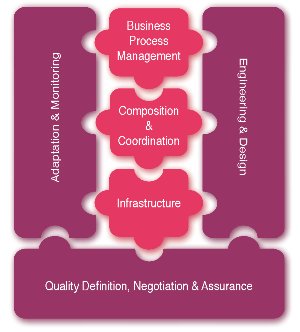
\includegraphics[width=.5\textwidth]{part1/pics/scube-overview.png}
  \caption{S-Cube Research Framework}
  \label{fig:scube-overview2}
%	\vspace{0.2cm}  
\end{wrapfigure}
S-Cube~\footnote{http://www.s-cube-network.eu/} is a European Network of Excellence (NoE) in Software, Services and Systems (S\up{3}). This NoE aims at making European research the leader in the software-services revolution. By connecting research to industry, and unifying multidisciplinary researches, S-Cube aims to develop agile and holistic service engineering methods, and to specify principles and techniques of service adaptation.\\
This European NoE has been funded by the European FP7 'Coordination' Research Programme  under the ICT theme. Along with strong collaboration and mobility opportunities beyond European research centers, S-Cube has funded several PhD theses in different layers of the S-Cube "BigPicture" (fig.~\ref{fig:scube-overview2}).\\

The skills of excellence of the INRIA Triskell team in which this theses was conducted, are dedicated to ease, and improve, software development methods, by the use of components, services, models and validations. Thanks to this team orientation, Triskell is involved in the S-Cube NoE, which has brought funding for two PhD theses. The research leading to the results presented in this theses has received credits from the European Community’s Seventh Framework Programme FP7/2007-2013 under grant agreement 215483 (S-Cube).\\

\subsection{Contribution}

The contribution of this thesis is aligned with the Work Package 1.2 : {\it Adaptation and Monitoring Principles, Techniques and Methodologies for Service-based Systems} of the Joint Research Activity(JRA) 1 : {\it Engineering and Adaptation Methodologies for Service-based Systems}\\

The general objective of the JRA-1, is to "devise an integrated set of principles, techniques and methodologies for engineering, adapting and monitoring hybrid service-based applications, while guaranteeing end-to-end quality provision and SLA conformance", according to the S-Cube description of work\footnote{DoW Amendment 4, December 6th, 2010}.\\
This thesis provides a new component model that: implies new engineering techniques and methodology, enables the adaptation of hybrid service-based application and offers means to perform checks and verifications to ensure the quality of services.\\

More precisely, the contribution of this thesis takes part in the JRA-1.2 work package, which aims to define novel principles and techniques for cross-layer monitoring and adaptation of Service-based Applications. If \enti{} does not address monitoring issues, it actually copes with adaptation requirements.\\

From the S-Cube perspective, \enti{} can be considered for handling adaptations of the infrastructure, or of the composition and coordination layer (see figure~\ref{fig:scube-overview}). Coupled with other layers, it can take part in the cross-layer adaptation mechanism.







\chapter{Scientific perspectives}

The contributions of this thesis leave some questions open, and have opened some doors. Therefore, the perspectives of this work aim at investigating and answering questions that have not been yet addressed, or go one step beyond into new uses of this contribution.


\section{IDA, second phase}
Conclusions from the experimentation led in the context of the \gls{ida} project shaped a promising future for the use of such tools, in the AAL domain. Even if the maturity of \enti{} and the objective of the first phase of the project did not allow testing of \enti{} in a real deployment situation, the protagonists (industrialists, carers, social workers and elderly people) have shown an interest in the provision of customized solutions for each person.\\
Currently, the second phase if the IDA project is being set up. Hopefully, it will be the moment for \enti{} to perform the last checks and to validate both the scalability and variability management, on real deployment.


\section{End User Programming}

End User Programming~\cite{Ko:2011} relates to the ability for anybody to program something. For instance, when a user programs the hours of start and stop of the heating system, he is actually programming. In the context of the IDA project and following the idea that inhabitants must be able to keep control of things in their homes, end user programming sounds like a very promising, but yet challenging perspective.\\

\subsection{Which description language ?}
Software developers like to be able to use the keyboard only. A graphical user interface, with drag-and-drop interactions to create assemblies, will probably not meet the requirements of this kind of population. For them, a textual language seems to be the simplest thing.\\
On the other hand, inhabitants do not all have skills in programming languages, and especially not elderly people. They would probably express their requirements for the behavior of the system in another way. The question is which one.\\

We had a range of description tools at our disposal, from a textual domain-specific language to a visual language composed of icons and boxes, linked with arrows. A solution for this problem probably lies somewhere in between these two extreme proposals and is surely not unique. Indeed, for the same system, an elderly person will probably be lost in a textual language and an engineer may be frustrated at being unable to express himself as usual.\\

The validity of the behavior described is also challenging. End users may not have a global vision of the system and thus may ask for a behavior that could lead the system to failure. Secondly, people naturally express the nominal behavior, without being concerned about possible deviations of this behavior. To address this problem, tools have to be proposed to check the validity of the nominal behavior and track and check any possible variation in the scenario.\\

The unique and universal language for describing how things have to behave will probably never exist. Because each user has a different kinship with technologies, systems should offer several edition tools, out of which the end user selects the handiest for him.


\subsection{Fuzzy Logic and Learning Algorithms}

In the hypothesis that people are able to describe a behavior of a function, how could they know about the limits of values? In other words, if a user is defining a behavior for the light, how could he know the minimum and maximum values that the light sensor can sense ?\\
The fuzzy logic paradigm~\cite{Chauvel:2008,Mendel:2001} proposes to use terms and non-fixed values in decision algorithms. Indeed, a fixed value is never appropriate because a regulation value must be modifiable. This paradigm makes it possible to work with terms and rough values only, because thresholds are computed at runtime. During the execution, users can act on these thresholds by telling the system about good or bad situations. Quite close to ideas of artificial intelligence, this approach could be coupled with some learning mechanisms, to go a bit further and re-simplify description of an application behavior.

\section{Distribution and Pervasiveness}

The distribution of applications brings several interesting facilities, such as load balancing, or redundancy to cope with failures of system elements. This question has not been properly addressed in this thesis, but may rapidly become a limitation. Moreover, working with devices brings \enti{} close to the ideas of pervasive computing. In this domain, objects' interactions are controlled by invisible nested software systems. Invisible for users, these systems have to self-reconfigure to take into account changes in their environments.\\

In the perspective of a large-scale deployment, distribution and pervasiveness can both come out as key requirements for some deployments. In \cite{Devescovi:2007}, Devescovi et al. propose algorithms for the self-organization of autonomic systems using the SelfLet approach. According to the presentation web page\footnote{http://selflet.sourceforge.net/}, a SelfLet is a "self-sufficient piece of software which is situated in some kind of logical or physical network, where it can interact and communicate with other SelfLets". This definition is very close to the definition of a smart device and SelfLets could be included in devices and device-controllers, such as firmware, to ease their integration.\\
This approach could foster the distribution of \enti{} on several nodes, help to prevent system failures, balance the load of resource-consuming components, or ease the connection of smart devices.


\section{Architecture Synthesis}
\label{sec:archiSynth}

The architecture synthesis goal is to assist in the creation of an application. Feature diagrams and automatic derivations into products, templates and wizards guiding the developer through the steps of product design, are two examples of tools enabling the synthesis of architectures.

\subsection{Dynamic Software Product Lines for the management of variability}

Not really addressed in the contribution, nor experimented in the validation, the management of variability in the domain of AAL and Home Automation is still a real problem. Luckily, the omnipresence of the model in all steps of the application-making process enables the use of well-known modeling tools to help in handling variability.\\

As proposed in~\cite{Morin:2010}, Aspect-Oriented Programming, coupled with Software Product Lines can be used to address this problem. Product Lines, a well-known variability management tool for supply chains, has been transposed into the software domain under the name of \gls{spl}. Large scale productions such as that of cars handles the variability of customers' requests using these product lines.\\
A product line consists of a base product that can be augmented with options selected by the customer. Software systems with a huge number of variable elements, such as component-based applications, can be defined the in the same way. The base functionalities of the software are described in the base product and specific options are plugged in according to the customer selection. The problem is that these tools have been set up to ease the one-shot creation of a product.\\

Dynamically-adaptive software systems are able to dynamically evolve after their creation, and \gls{spl}s are no longer sufficient to help in handling the description of things that can be changed at runtime. To cope with this issue, \gls{dspl} have been proposed. They enable the description of variation points during the execution of an application and make it possible to identify the exchangeable elements. The work carried out by Carlos Cetina et al. in this domain, presented in \cite{Cetina:2009}, is very close to what we want to achieve and reflects our future work.\\


\subsection{How can the behavior be descibed?}

In \enti{}, mapping components to leaf features in the \gls{dspl} makes it very simple to describe the desired configuration of the software at a high level of abstraction. Nevertheless, components in \enti{} are developed with a strong effort to respect the close entity principle and they do not know, or depend on each other. As a consequence, the \gls{dspl} can only support the description of the number of components, their types and the different options in the case of reconfiguration; in short, the structure of the assembly. Nowhere can the interactions between components be specified.\\

While still in its infancy, we proposed in~\cite{Istoan09a} an approach combining \gls{dspl} and Business Process Modeling. It enables the description of both architecture and behavior, by a combination of two modeling tools. Once coupled, these two models describe the structure of the application and its required behavior, which makes it possible to generate the entire system with connected components. As work in progress, this approach still has to be experimented in more depth.\\
Cassou et al. recently presented another approach to this problem of describing interactions. In \cite{Cassou:2011}, they introduce a "behavioral contract". These contracts are aimed at offering means to express the set of allowed interactions between components and describe both data and control-flow constraints. The integration of this idea with \enti{} may be studied in future work.


\section{Kevoree}

\enti{}, as an achievement of this thesis, has been highlighted as an interesting approach to address some identical issues in other domains.\\

For the principles of this contribution to be used in other contexts, \enti{} has recently been re-designed to become the customization of a more generic tool, specialized for home automation and AAL. Its name is Kevoree\footnote{http://kevoree.org}. The core mechanisms of adaptation, evolution, etc. have been moved into Kevoree in order to make them available for use cases other than home automation.\\

Whereas \enti{} is responsible for providing a set of services and components for Home Automation and AAL, Kevoree offers a set of tools for the component model. These include a framework to ease the implementation of components, a graphical editor to create component assemblies and a specialized runtime.\\
The development of Kevoree is actually part of the work in progress in the context of another thesis, which explores different improvements. For instance, questions about distribution and meanings of links between components.\\

{\bf Kermeta} is a \gls{dsl} optimized for metamodeling engineering. Developed in the TRISKELL team, it provides an integrated environment for Model-Driven engineering activities. Initially developed as a set of plugins for Eclipse, a work in progress is trying to make it run using the Kevoree tools.\\

{\bf Arduino} is an open-source electronics prototyping platform based on flexible, easy-to-use hardware and software. It is intended for artists, designers, hobbyists and anyone interested in creating interactive objects or environments, according to the manufacturer's web page. Recent developments shaped the idea of using Kevoree and the component model to ease sketches and the deployment of applications on Arduino platforms.


\section{Open Control/Command Operating System}

The component model of this contribution has been designed to allow for the connection of heterogeneous components. Inspired by electronics, the elements to be modeled and connected just need to be expressed in terms of components with inputs and outputs. Since almost all automated systems can be expressed this way, almost all systems can be modeled using the component model proposed in this contribution.\\
The independence of the model in relation to real devices-specificities enables the description of any application/system. Thus, \enti{} could take on the role of a universal control/command operating system, since the only difficult point is to develop the driver in charge of the interface between the real world and the component level. If a driver for an application can be created, \enti{} can help in controlling it.


\chapter{Industrial perspectives}
\label{ch:industrialPerspectives}

The contribution of this thesis interests several audiences. The general public is curious to know about how computer science can help in improving elderly people's quality of life at home, since \enti{} was initially designed for the Ambient Assisted Living context. Everyone has or has had a family member who could have been helped by such a proposal. Industrialists are more interested in the good properties of the contribution. Since device manufacturers are familiar with electronic components, they easily understand how this component model works.\\
Starting from the validation scenario, in just 3 years a demonstration of \enti{} has been set up and presented in more than 10 public and scientific events. This demonstration stressed the adaptation aspect of the contribution in an AAL context.

\section{Public events}

Public events are an opportunity for the general public to discover what issues scientists are trying to resolve and how they do it. On the other hand, these meetings are also an opportunity for scientists to collect feedback on their work, from uninitiated persons. Uninitiated, in the sense that they are thinking about the problem for the first time. The questions asked are often very interesting, prompting you to step back from the details and to consider the proposal from a more global view.\\

The most important presentation was probably the science festival held in 2009 in Rennes, where \enti{} had been selected to represent the INRIA laboratory. The science festival, {\it Fêtes de la Science}\footnote{See the videos (in French) at http://videos.rennes.inria.fr/fete-sciences-2009/index.html} in French, is a national event lasting for 3 days. From Friday to Sunday inclusive, scientists present their everyday work, explain the problems solved, or the phenomenon involved in some experiments.

\begin{figure}
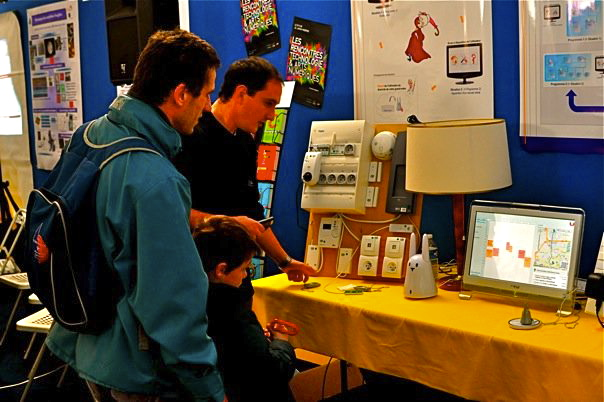
\includegraphics[width=\textwidth]{part4/pics/fdls.jpg}
\caption{Science festival presentation}
\end{figure}

During the first day, the festival admits only primary and middle school children. Visits are organized by groups and presenters have to explain their work to people aged from 7 to 15 years. This day is the most difficult day of the all festival. Not because the questions are complicated to answer, but because the explanation must be understood by everyone. This first day did not bring a lot of useful comments, or in any case, less than the two other days.\\

On Saturday and Sunday, the festival is open, for free, to families and anybody interested in sciences. These two days were a hard test for \enti{} and full of interesting discussions with people. Indeed, \enti{} had to run from 8am to 8pm without failure, disregarding touch-screen stress due to children's fingers, and in spite of the unpredicted use cases requested live by visitors.\\
It was the place for \enti{} to become enriched by new ideas, remarks, or people's experiences in facing elderly people's dependency problems. For the entire duration of the festival, no once did somebody say that \enti{} was useless, meaningless, or that the use case was not realistic. "It is not always that simple in real life" is the only remark we got.\\

Open days of the University of Rennes 1, or the opening celebration of the ESIR, the newly created engineering school of the University of Rennes 1, have also been two moments for exchanges with a large audience. Concerned by the studies, visitors' questions during these two events were more precise and more focused on what had been realized and how.\\
These demonstrations were sources of very interesting ideas to improve \enti{}.\\

Public presentations are very good opportunities to sense how the contribution exposed is perceived by anonymous people. None of them had a negative vision of the work, some had doubts and others asked about how to buy it. In my opinion it validates the utility of this contribution as perceived by people.\\

\enti{} has also been used as support for a demonstration called "{\it Leveraging Models From Design-time to Runtime. A Live Demo}" described in\cite{Morin09e}.

\section{Industrial perspectives}

The success of \enti{} has generated some industrial contacts. Several companies were interested in the abilities of this software to adapt and evolve at runtime. Most of them, close to the home automation domain, saw in \enti{} a great opportunity to enrich their products. But \enti{} was just a proof of concept, a prototype of research not ready to be deployed in the industry. This is partly the reason why \enti{} was not selected to be deployed in homes, in the IDA project.\\

Aware of this problem, a project of developing \enti{}, to make it ready for use in the industry had been submitted to the Regional Council of Brittany and accepted. This project funded the work of an engineer for one year, whose task was twofold. Firstly, to redevelop some parts of the contribution for it to be more stable, and secondly, to support the promotion of \enti{} in the industry. The development methods of \enti{} have been clarified and a second demonstration has been set up to focus more on the core functionalities and less on the home automation/AAL aspect.\\

In addition, a project of company creation is currently in progress and should end with the creation of a structure in charge of the promotion and support of \enti{} in the next few months. It was also a part of the development engineer's work to support the creation of this spin-off. 









%\bookmarksetup{startatroot}


%%------------%%
%%            %%
%%  ANNEXES   %% 
%%            %%

%%------------%%


\apendix


\clearpage

\printglossaries
\addcontentsline{toc}{part}{Acronyms}

%%------------%%
%%            %%
%%  BIBLIO    %% 
%%            %%
%%------------%%

\clearpage
\phantomsection
\addcontentsline{toc}{part}{Bibliography}
\bibliographystyle{alpha}
\bibliography{SE4IOT}


%%------------------%%
%%                  %%
%%  INDEX/TABLES    %% 
%%                  %%
%%------------------%%
%
%\newpage
%\cleardoublepage
%\addcontentsline{toc}{chapter}{Table des matières}
%\markboth{Table des matières}{Table des matières}
%\sommaire[2]
%\shorttableofcontents{Table des matières}{2}
%\tableofcontents{Table des matières}
%
%\bookmarksetup{startatroot}

\clearpage

\newpage
\cleardoublepage
\markboth{Table of figures}{Table of figures}
\listoffigures
\phantomsection
\addcontentsline{toc}{part}{Table of figures}


%%
%%\newpage
%%\cleardoublepage
%%\addcontentsline{toc}{chapter}{Liste des algorithmes}
%%\markboth{Liste des algorithmes}{Liste des algorithmes}
%%\listofalgorithms
%%

%%\newpage
%%\cleardoublepage
%%\addcontentsline{toc}{chapter}{Index}
%%\markboth{Index}{Index}
%%\printindex


%\commentaire{%-------------------- debut commentaire -------------------
%% Il faut mettre le résumé sur la quatrième de couverture. 
%% Suivant que votre liste de figures comporte un nombre pair 
%% ou impair de pages il faudra mettre un nombre pair ou impair
%% de commandes \newpage.

\backmatter

\clearpage

\lastpage

\alignquatriemedecouv
\phantomsection
\addcontentsline{toc}{part}{Summary}
\selectlanguage{frenchb}
\section*{R\'esum\'e}
Les systèmes logiciels tendent à se doter de facultés d’adaptation, d’évolution et d’ouverture. Ces capacités requièrent une grande flexibilité et dynamicité de l’environnement d’exécution, ainsi que de nouveaux outils d’assistance à la fabrication de ces systèmes. En électronique, des outils ont été déployés pour faire face à l’hétérogénéité et au nombre de composants, ainsi qu’aux besoins d’adaptation de produits existants à de nouvelles technologies. L’ouverture de la documentation et des spécifications a permis une grande richesse de solutions venant tant de bricoleurs que d’industriels.
Inspiré par l’électronique, cette thèse contribue à l’amélioration de la flexibilité des systèmes logiciels tout en conservant un haut niveau de fiabilité. Les apports se font à trois niveaux.\\
(1) Un nouveau modèle de composants qui offre une grande flexibilité et permet la connection de composants hétérogènes. \\
(2) Des outils issus de l’ingénierie des modèles, pour créer, modifier, simuler et valider la structure et le comportement des assemblages de composants avant leur déploiement. \\
(3) Un environnement d’exécution bati sur une architecture à base de services, pour supporter les évolutions, les adaptations et l’ouverture requises par le modèle de composant proposé.\\
Cette thèse a été validée sur un cas concret dans un projet d’aide à domicile. Dans ce domaine, les systèmes logiciels doivent être adaptables et flexibles, pour répondre aux évolutions des besoins et pathologies des personnes âgées. Les bénéfices acquis de l’utilisation de cette approche dans ce contexte ont prouvé la pertinence de cette thèse.



\selectlanguage{english}
\section*{Abstract}

Software systems tend to acquire capabilities of adaptation, evolution and openness. These abilities require the execution environment to be highly flexible and dynamic, and require new tools to handle these abilities. In electronics, tools have been set up to cope with the huge heterogeneity and number of components, and the adaptation of existing products to new technologies. Openness of documentations and specifications in this area led to a wealth of solutions made by industrials or individuals fond of electronics.\\
Inspired by electronics' achievements this thesis contributes in improving the flexibility of software systems while maintaining a high level of reliability. The contribution is threefold. (1) A new component model, which improves flexibility to enable connection of heterogeneous components. (2) Tools from model driven engineering, to create, edit, simulate and validate the structure and behavior of component assemblies prior to their (re-)deployment. (3) A runtime environment built on top of a service-based architecture to support evolutions, adaptations and openness required by the proposed component model.\\
This thesis has been validated on a use case from an Ambient Assisted Living project. In this domain, software systems have to be adaptive and flexible, to fit the needs and pathology evolutions of elderly people. Although there still is a long way to go, the benefits gained from the use of this approach in this context proved the relevance of this thesis.

\end{document}
















